\documentclass[a4paper,12pt]{book}

% Pakker til bedre udseende og funktionalitet
\usepackage[utf8]{inputenc}
\usepackage[T1]{fontenc} % Bedre skrifttyper til specialtegn
\usepackage[danish]{babel}
\usepackage{graphicx}
\usepackage{amsmath}
\usepackage{amssymb} % Tilføjer flere matematiksymboler
\usepackage{hyperref}
\usepackage{lipsum} % Tilføjer dummy-tekst til eksempler
\usepackage{caption} % Bedre kontrol over billedtekster
\usepackage{fancyhdr}
\pagestyle{empty}  % Dette deaktiverer sidehoveder og sidefødder på alle sider


% Titel og forfatter
\title{Trådløs Kommunikation: Path Loss og Shadowing}
\author{Forfatterens Navn}

\begin{document}
	
	% Titelside
	\maketitle
	\tableofcontents
	\clearpage
	
	\chapter{Path Loss and Shadowing}
	Den trådløse radiokanal udgør en betydelig udfordring som medium for pålidelig højhastighedskommunikation. Ikke alene er kanalen udsat for støj, interferens og andre forstyrrelser, men disse forhindringer ændrer sig også over tid på uforudsigelige måder som følge af brugerens bevægelse. I dette kapitel vil vi karakterisere variationen i modtaget signalstyrke som en funktion af afstanden mellem sender og modtager, med fokus på de primære faktorer: path loss og shadowing.
	\newline\newline\noindent
	Path loss opstår, når signalets energi gradvist aftager, efterhånden som det bevæger sig væk fra senderen. Denne dæmpning skyldes primært den fysiske udbredelse af signalets energi over et større område og påvirkninger fra selve udbredelseskanalen. Modeller for path loss antager generelt, at tabet er ens for en given afstand mellem sender og modtager.
	\newline\newline\noindent
	Shadowing forekommer, når forhindringer som bygninger, træer eller bakker dæmper signalstyrken. Disse forhindringer kan påvirke signalet gennem mekanismer som absorption, refleksion, spredning og diffraktion. Når dæmpningen er særlig kraftig, kan signalet blive helt blokeret.
	
	\section{Variationer i Signalstyrke: Path Loss, Shadowing og Multipath}
	Når et signal transmitteres i et trådløst miljø, vil det opleve forskellige typer af dæmpning afhængigt af både afstanden mellem sender og modtager og de specifikke forhold i miljøet. Disse dæmpninger påvirker forholdet mellem den transmitterede effekt \( P_t \) og den modtagne effekt \( P_r \).
	
	\subsection{Path Loss og Shadowing}
	\textbf{Path Loss:} Path loss opstår typisk over lange afstande, eksempelvis mellem 100 og 1000 meter. Denne effekt beskriver den gradvise reduktion i signalstyrke, der sker, når signalet bevæger sig længere væk fra senderen. Path loss skyldes primært, at signalets energi spredes over et større område, hvilket medfører et energitab per enhedsområde.
	\newline\newline\noindent
	\textbf{Shadowing:} Shadowing opstår, når signalet passerer gennem eller omkring forhindringer, der forårsager yderligere dæmpning. Disse variationer i signalstyrken sker over kortere afstande, der svarer til størrelsen af de hindrende objekter, typisk mellem 10 og 100 meter i udendørs miljøer, og endnu kortere i indendørs miljøer.
	\newline\newline\noindent
	Da både path loss og shadowing ændrer signalstyrken over relativt store afstande, betegnes disse effekter ofte som \textit{large-scale propagation effects}.
	
	\subsection{Multipath Effekter}
	\textbf{Multipath:} Ud over path loss og shadowing kan signalet også påvirkes af \textit{multipath} effekter, som opstår, når signalet reflekteres af forskellige objekter i miljøet og dermed når frem til modtageren via flere veje. Disse refleksioner kan forårsage både konstruktiv og destruktiv interferens, hvilket skaber hurtige variationer i signalstyrken over meget korte afstande, ofte på størrelse med signalets bølgelængde. Disse variationer kaldes \textit{small-scale propagation effects}.

	\begin{figure}[h]
		\centering
		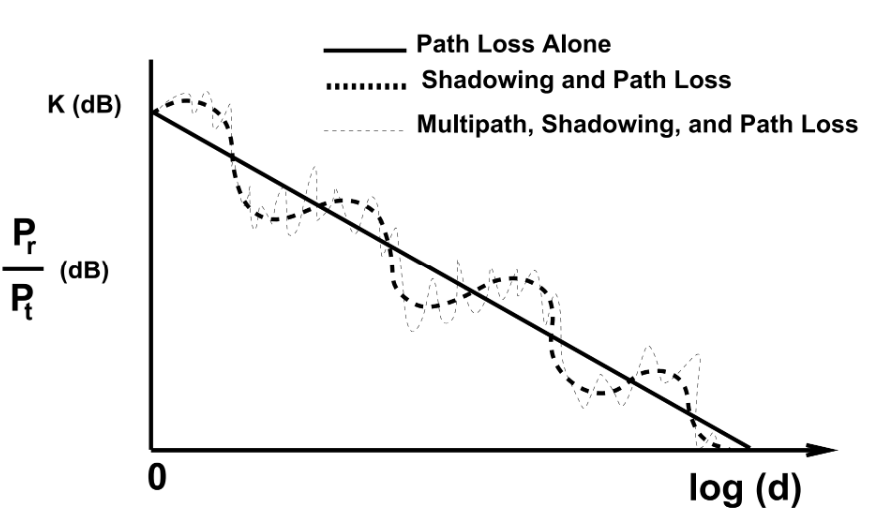
\includegraphics[width=0.6\textwidth]{fig/fig1.png}
		\caption{Path Loss, Shadowing og Multipath versus Distance.}
		\label{fig:path_loss_shadowing}
	\end{figure}
	
	\noindent Figur \ref{fig:path_loss_shadowing} viser forholdet mellem modtaget effekt (\(P_r\)) og transmitteret effekt (\(P_t\)) som en funktion af afstand (log(d)) i dB. Den fuldt optrukne linje repræsenterer effekten af path loss alene, den stiplede linje inkluderer effekterne af både path loss og shadowing, og den prikkede linje viser, hvordan multipath effekter kan skabe yderligere variationer. Figuren illustrerer, hvordan signalstyrken gradvist reduceres med øget afstand, og hvordan shadowing og multipath kan forårsage yderligere udsving i signalstyrken.	
	
	\section{Radio Wave Propagation}
	Den første forståelse af, hvordan radiobølger bevæger sig, stammer fra det banebrydende arbejde udført af James Clerk Maxwell i 1864. Maxwell udviklede teorien om elektromagnetiske bølger, som forudsagde, at radiobølger eksisterer. I 1887 beviste Heinrich Hertz eksperimentelt, at disse bølger faktisk eksisterer. Hertz mente dog, at radiobølger ikke havde nogen praktisk anvendelse, da han troede, at de ikke kunne bruges til at overføre stemme på grund af deres lave frekvens og dårlige udbredelse. Maxwells og Hertz' arbejde lagde grundlaget for radiokommunikation: i 1894 brugte Oliver Lodge disse principper til at skabe det første trådløse kommunikationssystem, selvom det kun kunne sende signaler op til 150 meter. I 1897 lykkedes det Guglielmo Marconi at sende et radiosignal fra Isle of Wight til en båd 18 miles væk, og i 1901 kunne hans system sende signaler over Atlanterhavet. Disse tidlige systemer brugte telegrafsignaler til at overføre information. I 1906 blev den første transmission af stemme og musik gennemført af Reginald Fessenden ved hjælp af amplitude modulation, hvilket omgåede de begrænsninger ved lave frekvenser, som Hertz havde påpeget, ved at flytte signalerne til en højere frekvens – en metode, der stadig anvendes i moderne trådløse systemer.
	\newline\newline\noindent
	Elektromagnetiske bølger bevæger sig gennem forskellige miljøer, hvor de kan reflekteres, spredes og brydes af forhindringer som vægge, terræn og bygninger. For at forstå disse processer i detaljer kan man bruge Maxwells ligninger, der kræver kendskab til de fysiske egenskaber af de objekter, som bølgerne interagerer med. Dette kan involvere komplekse beregninger af radar tværsnitsarealet (RCS) for store strukturer. Da disse beregninger ofte er svære og kræver data, som ikke altid er tilgængelige, benyttes der ofte tilnærmelsesmetoder til at beskrive signaludbredelse uden at skulle løse Maxwells ligninger.
	\newline\newline\noindent
	En af de mest anvendte tilnærmelser er strålesporingsteknikker. Disse metoder simplificerer udbredelsen af elektromagnetiske bølger ved at behandle bølgefronter som simple partikler. Modellen kan beskrive refleksioner og brydninger, men den ignorerer de mere komplekse spredningseffekter, som Maxwells ligninger forudsiger. En simpel strålesporingsmodel er tostrålemodellen, som beskriver udbredelsen, når der er én direkte vej mellem senderen og modtageren samt én reflekteret vej, typisk fra jorden. Denne model er god til at beskrive signaludbredelse langs motorveje, landeveje og over vand. Mere komplekse modeller overvejes også, hvor flere refleksioner, spredninger og brydninger inddrages. Mange miljøer kan dog ikke beskrives præcist med strålesporing alene. I disse tilfælde anvendes analytiske modeller baseret på empiriske målinger, og vi vil se på nogle af de mest almindelige empiriske modeller.
	\newline\newline\noindent
	Ofte er radiokanalens kompleksitet og variationer så store, at det er svært at opnå en nøjagtig deterministisk model. I sådanne tilfælde benyttes statistiske modeller ofte. Dæmpning forårsaget af hindringer som bygninger eller andre objekter beskrives typisk statistisk. Statistiske modeller bruges også til at beskrive den konstruktive og destruktive interferens fra mange multipath-komponenter. Disse modeller er mest præcise i miljøer med regelmæssige geometrier og ensartede dielektriske egenskaber. Indendørs miljøer har ofte mere uregelmæssige forhold end udendørs miljøer, da både geometri og dielektriske egenskaber kan variere betydeligt, afhængigt af om miljøet er en åben fabrik, kontor eller værksted. For sådanne miljøer er computerbaserede modelleringsværktøjer tilgængelige for at forudsige, hvordan signalerne udbredes.
	
	\section{Transmitterede og Modtagede Signaler}
	For at forstå modellerne for transmissions- og modtagesignaler i trådløse kommunikationssystemer, er det nødvendigt at starte med en beskrivelse af, hvad et signal er, og hvordan det påvirkes, når det passerer gennem en kommunikationskanal.
	
	\subsection{Transmitteret Signal}
	Vi modellerer det transmitterede signal \( s(t) \) som den reelle del af et komplekst signal:
	
	\[
	s(t) = \Re \{ u(t) e^{j2\pi f_c t} \}
	\]
	
	\noindent hvor \( u(t) \) er et komplekst basbåndssignal defineret som:
	
	\[
	u(t) = x(t) + jy(t)
	\]
	
	\noindent Her er \( x(t) \) den reelle komponent (in-phase) af basbåndssignalet, og \( y(t) \) er den imaginære komponent (kvadraturkomponenten). Disse komponenter har båndbredden \( B_u \) og effekten \( P_u \).
	
	\noindent Det komplekse basbåndssignal \( u(t) \) kan også skrives som:
	
	\[
	s(t) = x(t) \cos(2\pi f_c t) - y(t) \sin(2\pi f_c t)
	\]
	
	\noindent hvor \( f_c \) er bærefrekvensen.
	
	\noindent Signalet \( u(t) \) kaldes den \textit{komplekse kuvert} eller det \textit{komplekse lavpasækvivalente signal} for \( s(t) \). Dette navn kommer af, at \( |u(t)| \) repræsenterer amplituden, og argumentet af \( u(t) \) repræsenterer fasen af \( s(t) \).
	
	\subsection{Modtaget Signal}
	Det modtagede signal \( r(t) \) modelleres på samme måde:
	
	\[
	r(t) = \Re \{ v(t) e^{j2\pi f_c t} \}
	\]
	
	\noindent hvor \( v(t) \) er det komplekse basbåndssignal, der afhænger af den kanal, signalet transmitteres igennem. Hvis \( s(t) \) transmitteres gennem en tidsinvariant kanal, vil \( v(t) = u(t) * c(t) \), hvor \( c(t) \) er kanalens impulsrespons.
	
	\subsection{Doppler Effekt}
	Når modtageren bevæger sig i forhold til senderen, opstår en Doppler-forskydning, som resulterer i en frekvensskift \( f_D \) givet ved:
	
	\[
	f_D = \frac{1}{2\pi} \frac{\Delta \phi}{\Delta t} = \frac{v \cos \theta}{\lambda}
	\]
	
	\noindent hvor \( v \) er modtagerens hastighed mod senderen, \( \theta \) er vinklen mellem signalretningen og bevægelsesretningen, og \( \lambda = \frac{c}{f_c} \) er signalets bølgelængde.
	
	\subsection{Path Loss}
	Når et signal transmitteres gennem en given kanal, tabes noget af signalets effekt undervejs, hvilket kaldes \textit{path loss}. Dette tab kan udtrykkes som forholdet mellem den transmitterede effekt \( P_t \) og den modtagede effekt \( P_r \):
	
	\[
	P_L = \frac{P_t}{P_r}
	\]
	
	\noindent Dette kan også udtrykkes i dB som:
	
	\[
	P_L \, \text{dB} = 10 \log_{10} \left( \frac{P_t}{P_r} \right) \, \text{dB}
	\]
	
	\noindent Heraf kan man også definere \textit{path gain} \( P_G \) som:
	
	\[
	P_G = -P_L = 10 \log_{10} \left( \frac{P_r}{P_t} \right) \, \text{dB}
	\]
	
	\noindent Disse begreber bruges til at karakterisere, hvor meget signalstyrken reduceres eller forøges, når signalet bevæger sig gennem kommunikationskanalen.
	
	\chapter{Free-Space Path Loss og Doppler-effekt}
	\label{cha:Free-Space Path Loss og Doppler-effekt}
	\section{Free-Space Path Loss og Doppler-effekt}
	
	\subsection{Free-Space Path Loss}
	Når et signal transmitteres gennem fri luft fra en sender til en modtager uden nogen forhindringer imellem, beskriver vi transmissionen som værende over en line-of-sight (LOS) kanal. Den modtagne signalstyrke \( P_r \) i forhold til den transmitterede effekt \( P_t \) kan beskrives som:
	
	\[
	\frac{P_r}{P_t} = \left( \frac{\lambda}{4\pi d} \right)^2
	\]
	
	hvor:
	\begin{itemize}
		\item \( P_r \) er den modtagne effekt (W),
		\item \( P_t \) er den transmitterede effekt (W),
		\item \( \lambda = \frac{c}{f_c} \) er signalets bølgelængde (meter),
		\item \( d \) er afstanden mellem sender og modtager (meter),
		\item \( c \) er lysets hastighed (\(3 \times 10^8 \, \text{m/s}\)),
		\item \( f_c \) er bærefrekvensen (Hz).
	\end{itemize}
	
	Free-space path loss (FSPL) beskriver den signalstyrketab, der opstår som følge af, at signalet spredes i rummet, og kan også udtrykkes i decibel (dB) som:
	
	\[
	P_L \, \text{(dB)} = 20 \log_{10} \left( \frac{4\pi d f_c}{c} \right)
	\]
	
	Denne ligning viser, at path loss stiger logaritmisk med både afstanden \( d \) og bærefrekvensen \( f_c \). Path loss øges med øget afstand og højere frekvenser, hvilket resulterer i en lavere modtaget effekt.
	\newline\newline\noindent
	\textbf{Teori:}
	Free-space path loss-modellen antager en ren LOS mellem sender og modtager uden nogen former for refleksioner, absorptioner eller forhindringer. Modellen bruges i satellitkommunikation og trådløse kommunikationsscenarier, hvor der ikke er nogen væsentlige forhindringer mellem sender og modtager.
	
	\subsection{Doppler-effekt}
	Når enten senderen eller modtageren bevæger sig, oplever vi en frekvensændring på grund af Doppler-effekten. Doppler-frekvensforskydningen \( f_D \) beskriver forskellen mellem den transmitterede frekvens \( f_c \) og den modtagne frekvens, og den kan beregnes som:
	
	\[
	f_D = \frac{v \cos \theta}{\lambda}
	\]
	
	hvor:
	\begin{itemize}
		\item \( v \) er hastigheden af modtageren i forhold til senderen (meter/sekund),
		\item \( \lambda \) er signalets bølgelængde (meter),
		\item \( \theta \) er vinklen mellem bevægelsesretningen og signalets udbredelsesretning.
	\end{itemize}
	
	\noindent Når modtageren bevæger sig mod senderen, vil \( f_D \) være positiv (en højere frekvens modtages), og når modtageren bevæger sig væk fra senderen, vil \( f_D \) være negativ (en lavere frekvens modtages).
	\newline\newline\noindent
	\textbf{Teori:}
	Doppler-effekten opstår i bevægende modtagere eller sendere i forhold til hinanden, som f.eks. biler, der bevæger sig forbi radiostationer eller fly, der kommunikerer med en jordbaseret station. Dette påvirker den opfattede frekvens, og derfor er Doppler-effekten vigtig i mange mobile kommunikationsscenarier.
	
	\subsection{Eksempler}
	\subsubsection{Eksempel 1: Beregning af Free-Space Path Loss}
	\textbf{Problem:} Betragt en trådløs forbindelse, hvor en sender transmitterer en effekt \( P_t = 1 \, \text{W} \) ved en frekvens \( f_c = 2.4 \, \text{GHz} \). Afstanden mellem sender og modtager er \( d = 100 \, \text{m} \). Beregn den modtagne effekt \( P_r \), hvis både sender- og modtagerantennerne er isotropiske (dvs. \( G_t = G_r = 1 \)).
	\newline\newline\noindent
	\textbf{Løsning:}
	Vi starter med at beregne bølgelængden \( \lambda \):
	
	\[
	\lambda = \frac{c}{f_c} = \frac{3 \times 10^8 \, \text{m/s}}{2.4 \times 10^9 \, \text{Hz}} = 0.125 \, \text{m}
	\]
	\noindent
	Vi anvender nu ligningen for forholdet mellem den modtagne og den transmitterede effekt:
	
	\[
	\frac{P_r}{P_t} = \left( \frac{\lambda}{4\pi d} \right)^2
	\]
	\noindent
	Indsætter værdierne:
	
	\[
	\frac{P_r}{1 \, \text{W}} = \left( \frac{0.125 \, \text{m}}{4\pi \times 100 \, \text{m}} \right)^2 = \left( \frac{0.125}{1256.64} \right)^2 = 9.89 \times 10^{-10}
	\]
	\noindent
	Den modtagne effekt bliver:
	
	\[
	P_r = 1 \, \text{W} \times 9.89 \times 10^{-10} = 9.89 \times 10^{-10} \, \text{W} = 0.989 \, \text{nW}
	\]
	\noindent
	Omregnet til dBm:
	
	\[
	P_r \, \text{dBm} = 10 \log_{10}(0.989 \times 10^{-9}) \approx -90.05 \, \text{dBm}
	\]
	
	\subsubsection{Eksempel 2: Beregning af Doppler-Skift}
	\textbf{Problem:} Antag, at en bil bevæger sig med en hastighed \( v = 30 \, \text{m/s} \) mod en radiosender, der sender ved en frekvens \( f_c = 900 \, \text{MHz} \). Beregn Doppler-forskydningen \( f_D \), hvis bevægelsesvinklen \( \theta = 0^\circ \).
	\newline\newline\noindent
	\textbf{Løsning:}
	Doppler-forskydningen \( f_D \) beregnes som:
	
	\[
	f_D = \frac{v \cos \theta}{\lambda}
	\]
	\noindent
	Bølgelængden \( \lambda \) er:
	
	\[
	\lambda = \frac{c}{f_c} = \frac{3 \times 10^8 \, \text{m/s}}{900 \times 10^6 \, \text{Hz}} = 0.333 \, \text{m}
	\]
	\noindent
	Da \( \theta = 0^\circ \), bliver \( \cos \theta = 1 \), og derfor:
	
	\[
	f_D = \frac{30 \, \text{m/s}}{0.333 \, \text{m}} = 90 \, \text{Hz}
	\]
	\noindent
	Doppler-forskydningen er derfor \( 90 \, \text{Hz} \), og den modtagne frekvens ved modtageren bliver \( f_c + f_D = 900.090 \, \text{MHz} \).
	
	\subsubsection{Eksempel 3: Beregning af Free-Space Path Loss ved 1 km Afstand}
	\textbf{Problem:} Beregn path loss ved en afstand på \( d = 1 \, \text{km} \) ved en frekvens på \( f_c = 2.4 \, \text{GHz} \).
	\newline\newline\noindent
	\textbf{Løsning:}
	Free-space path loss i dB er:
	
	\[
	P_L \, \text{(dB)} = 20 \log_{10} \left( \frac{4\pi d f_c}{c} \right)
	\]
	
	Indsæt værdierne:
	
	\[
	P_L = 20 \log_{10} \left( \frac{4\pi \times 1000 \times 2.4 \times 10^9}{3 \times 10^8} \right) = 20 \log_{10} (100.48) \approx 100.04 \, \text{dB}
	\]
	
	Path loss ved 1 km afstand er derfor \( 100.04 \, \text{dB} \).
	
	
	\section{Ray Tracing}
	
	\noindent Forestil dig, at du kaster en bold i et rum fyldt med forskellige objekter som vægge, møbler og vinduer. Bolden vil ramme disse objekter og blive kastet tilbage i forskellige retninger. På samme måde, når et radiosignal (som en usynlig bølge) bliver sendt fra en sender i et bymiljø eller indenfor i en bygning, vil det støde på mange ting, der får signalet til at blive reflekteret, bøjet (diffracted), eller spredt. De ekstra signaler, som bliver skabt på denne måde, kaldes for \textit{multipath signal components}.
	\newline\newline\noindent
	Når disse multipath signaler når frem til modtageren, bliver de lagt sammen med det oprindelige signal. Dette kan resultere i, at det modtagne signal kan blive forvrænget (altså ændret i forhold til det oprindelige signal). 
	\begin{figure}[h]
		\centering
		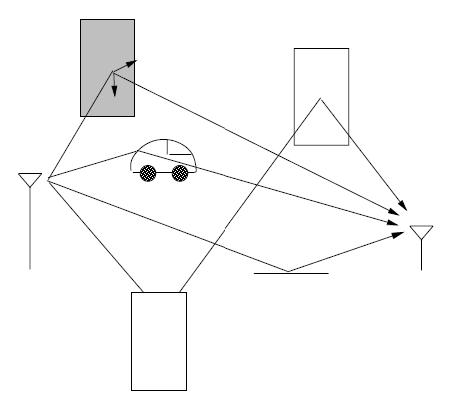
\includegraphics[width=0.6\textwidth]{fig/fig3.png}
		\caption{Reflected, Diffracted, and Scattered Wave Components.}
		\label{fig:ray_tracing}
	\end{figure}
	
	\noindent
	På billedet kan du se, hvordan et signal, der bliver sendt fra én kilde, kan reflekteres, bøjes, og spredes af objekter som bygninger, biler og vægge, før det når frem til modtageren.
	\newline\newline\noindent
	I \textit{ray tracing} antager vi, at der er et bestemt antal reflektorer (som de ting, signalet rammer) med kendte placeringer og egenskaber. Ved at bruge nogle ret avancerede ligninger, som Maxwell's ligninger, kan vi forudsige, hvordan signalet vil opføre sig, når det støder på disse objekter. Men disse beregninger kan være meget komplicerede og tage lang tid at udføre, så i praksis bruger vi ofte en forenklet metode, hvor vi behandler signalet som simple bølger, der bliver reflekteret, bøjet eller spredt.
	\newline\newline\noindent
	Denne metode fungerer bedst, når modtageren er langt væk fra den nærmeste genstand, og når genstandene, signalet rammer, er store sammenlignet med signalets bølgelængde.
	\newline\newline\noindent
	Hvis både senderen, modtageren og alle de ting, signalet rammer, ikke bevæger sig, så vil de \textit{multipath} signaler, der modtages, være ret stabile. Men hvis noget af det bevæger sig, vil disse signaler ændre sig over tid, og vi bliver nødt til at tage højde for det, når vi beregner, hvordan signalet vil se ud ved modtageren. I sådanne situationer bruger vi statistiske modeller for at forudsige, hvordan signalet vil opføre sig.
	\newline\newline\noindent
	De mest almindelige \textit{ray tracing} modeller inkluderer alle de reflekterede, bøjede og spredte signaler. Disse modeller bruger detaljerede oplysninger om både objekternes placering og deres fysiske egenskaber til at beregne, hvordan signalet vil opføre sig.
	\newline\newline\noindent
	Nogle populære computerprogrammer, som bruges til at planlægge trådløse systemer i både indendørs og udendørs miljøer, er \textit{Wireless Valley's SitePlanner®} og \textit{Marconi's Planet® EV}. Disse programmer kombinerer computergrafik med fotos eller tegninger af omgivelserne for at skabe et 3D-billede af miljøet.
	\newline\newline\noindent
	I praksis findes der flere forskellige \textit{ray tracing} modeller, som kan variere i kompleksitet:
	\begin{itemize}
		\item En simpel model, der forudsiger, hvordan et signal varierer på grund af en refleksion fra jorden.
		\item En mere avanceret model, der bruger op til ti refleksioner til at forudsige, hvordan et signal opfører sig langs en lige vej eller en gang.
		\item En generel model, der kan forudsige signaludbredelse i ethvert miljø.
	\end{itemize}
	Den enkle model kræver kun information om antennehøjder, mens de mere avancerede modeller også kræver detaljer om gadernes bredde i byområder eller gangenes bredde indendørs, samt om de objekter, der kan reflektere eller sprede signalet.
	
	\subsection{Two-Ray Model}
	
	\noindent Two-ray modellen bruges, når en enkelt refleksion fra jorden dominerer de multipath-effekter, som opstår, når signalet når frem til modtageren. I figur \ref{fig:two_ray_model} kan du se, hvordan signalet bevæger sig fra senderen til modtageren. Signalet opdeles i to dele: en direkte linje-of-sight (LOS) komponent, som er det direkte signal fra senderen, og en reflekteret komponent, som er signalet, der bliver reflekteret fra jorden.
	
	\begin{figure}[h]
		\centering
		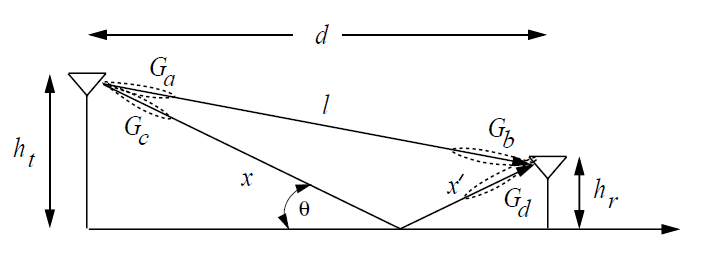
\includegraphics[width=0.8\textwidth]{fig/fig4.png}
		\caption{Two-Ray Model.}
		\label{fig:two_ray_model}
	\end{figure}
	
	\noindent
	Det modtagne LOS-signal beregnes ved hjælp af free-space propagation loss formlen, som vi så tidligere. Det reflekterede signal vises i figur \ref{fig:two_ray_model} som segmenterne \(x\) og \(x'\). Hvis vi ser bort fra effekten af overfladebølgedæmpning, så kan vi beregne det modtagne signal i two-ray modellen ved at kombinere LOS og det reflekterede signal:
	
	\[
	r_{2ray}(t) = \Re \left\{ \frac{\lambda}{4\pi} \left[ \frac{\sqrt{G_l} u(t) e^{-j2\pi l/\lambda}}{l} + \frac{R \sqrt{G_r} u(t - \tau) e^{-j2\pi(x+x')/\lambda}}{x + x'} \right] e^{j2\pi f_c t} \right\}
	\]
	
	\noindent
	Her er \( \tau = \frac{(x + x' - l)}{c} \) tidsforskellen mellem refleksionen og LOS-signalet, og \( \sqrt{G_l} = \sqrt{G_a G_b} \) er produktet af senderens og modtagerens antennediagrammer i LOS-retningen. \( R \) er refleksionskoefficienten, og \( \sqrt{G_r} = \sqrt{G_c G_d} \) er produktet af senderens og modtagerens antennediagrammer svarende til strålerne af længde \(x\) og \(x'\).
	
	\noindent
	Hvis det transmitterede signal er smalbåndet i forhold til tidsforskellen \( \tau \ll B_u^{-1} \), så kan \( u(t) \approx u(t - \tau) \). Med denne antagelse kan den modtagne effekt i two-ray modellen for smalbåndstransmission skrives som:
	
	\[
	P_r = P_t \left[ \frac{\lambda}{4\pi} \right]^2 \left| \frac{\sqrt{G_l}}{l} + \frac{R \sqrt{G_r} e^{-j\Delta \phi}}{x + x'} \right|^2
	\]
	
	\noindent
	Her er \( \Delta \phi = \frac{2\pi(x + x' - l)}{\lambda} \) faseskiftet mellem de to modtagne signaler. Ligning (2.12) er vist at være i god overensstemmelse med empiriske data.
	
	\noindent
	Når \( d \) (afstanden mellem sender og modtager) er meget større end \( h_t + h_r \), kan vi bruge en Taylor-serie tilnærmelse for at forenkle \( \Delta \phi \) til:
	
	\[
	\Delta \phi \approx \frac{4\pi h_t h_r}{\lambda d}
	\]
	
	\noindent
	Reflektionskoefficienten \( R \) kan beregnes ved hjælp af ligning (2.15):
	
	\[
	R = \frac{\sin \theta - Z}{\sin \theta + Z}
	\]
	
	\noindent
	Hvor \( Z \) afhænger af polariseringen af signalet, og \( \epsilon_r \) er materialets dielektriske konstant. For jord eller vejoverflader er \( \epsilon_r \) typisk omkring 15.
	
	\noindent
	I det asymptotiske tilfælde, hvor \( d \) er meget stor, vil den modtagne effekt falde med den fjerde potens af \( d \):
	
	\[
	P_r \approx P_t \left[ \frac{\lambda \sqrt{G_l}}{4\pi d} \right]^2 \left[ \frac{4\pi h_t h_r}{\lambda d} \right]^2
	\]
	
	\noindent
	I decibel (dB) kan den modtagne effekt skrives som:
	
	\[
	P_r \, \text{dBm} = P_t \, \text{dBm} + 10 \log_{10}(G_l) + 20 \log_{10}(h_t h_r) - 40 \log_{10}(d)
	\]
	
	\noindent
	Således, når \( d \) bliver meget stor, falder den modtagne effekt med fjerde potens af afstanden \( d \) og er uafhængig af bølgelængden \( \lambda \). Det modtagne signal bliver i dette tilfælde uafhængigt af \( \lambda \), da kombinationen af den direkte sti og det reflekterede signal ligner effekten af et antennediagram, og retningsbestemte antenner har en modtaget effekt, som ikke nødvendigvis falder med frekvensen.
	
	\begin{figure}[h]
		\centering
		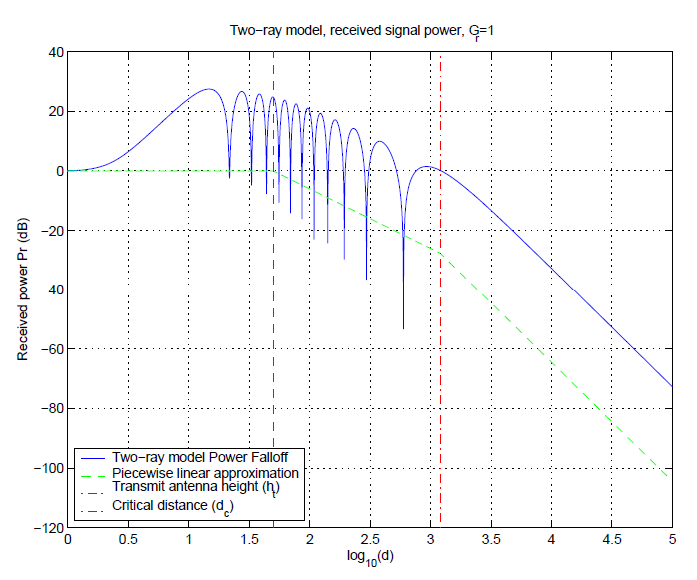
\includegraphics[width=0.8\textwidth]{fig/fig5.png}
		\caption{Received Power versus Distance for Two-Ray Model.}
		\label{fig:two_ray_falloff}
	\end{figure}
	
	\noindent
	Dette plot kan opdeles i tre segmenter. For små afstande (\( d < h_t \)) kombineres de to stråler konstruktivt, og path loss er nogenlunde flad. For moderate afstande, når \( d \) er proportional med \( \sqrt{d^2 + (h_t - h_r)^2} \), falder effekten med \( 1/(d^2 + h_t^2) \). For meget store afstande falder effekten med \( 1/d^4 \).
	
	\subsubsection{Kritisk Distance i Two-Ray Modellen}
	
	\noindent Den kritiske distance \( d_c \) i en two-ray model er afgørende for at bestemme, hvornår signalet fra den reflekterede stråle begynder at interferere signifikant med den direkte stråle. Denne distance kan beregnes ved hjælp af formlen:
	
	\[
	d_c = \frac{4h_t h_r}{\lambda}
	\]
	
	\noindent hvor:
	\begin{itemize}
		\item \( h_t \) og \( h_r \) er højderne på henholdsvis sender- og modtagerantennerne.
		\item \( \lambda \) er bølgelængden af signalet.
	\end{itemize}
	
	\noindent Når afstanden \( d \) mellem sender og modtager er større end \( d_c \), vil den modtagne signalstyrke falde hurtigt, hvilket kan have stor indflydelse på netværksplanlægning, især i byområder og indendørs miljøer.
	
	\subsubsection{Eksempel 2.2: Beregning af Kritisk Distance}
	
	\noindent I dette eksempel skal vi beregne den kritiske distance \( d_c \) for en bymæssig microcell (hvor \( h_t = 10 \) m og \( h_r = 3 \) m) og en indendørs microcell (hvor \( h_t = 3 \) m og \( h_r = 2 \) m) ved en frekvens \( f_c = 2 \) GHz.
	\newline\newline
	\noindent \textbf{Løsning:} Den kritiske distance \( d_c \) for en bymæssig microcell er 800 meter, mens den for en indendørs microcell er 160 meter. Disse afstande viser, at en celleradius på 800 m er for stor til et bymæssigt microcell system, hvor man typisk ønsker celler på omkring 100 m for at opretholde høj kapacitet. På samme måde er 160 m for stort til en indendørs microcell, hvor der typisk er mange vægge, som signalet skal passere igennem, hvilket kræver en mindre celleradius, omkring 10-20 m.
	
	\subsubsection{Eksempel 2.3: Beregning af Modtaget Effekt ved Forskellige Frekvenser}
	
	\noindent Beregn den modtagne effekt for en two-ray model, når sender- og modtagerhøjderne er \( h_t = 15 \) m og \( h_r = 2 \) m, og afstanden mellem dem er \( d = 500 \) m. Antag, at frekvensen \( f_c \) er henholdsvis 900 MHz og 2.4 GHz, og at antenneforstærkningen \( G_t = G_r = 1 \).
	
	\noindent \textbf{Løsning:} For 900 MHz beregnes den modtagne effekt ved:
	
	\[
	P_r \approx P_t \left[ \frac{\lambda}{4\pi d} \right]^2 \left[ \frac{4\pi h_t h_r}{\lambda d} \right]^2
	\]
	
	\noindent hvor \( \lambda = \frac{c}{f_c} = \frac{3 \times 10^8}{900 \times 10^6} = 0.333 \) m. Ved 2.4 GHz er \( \lambda = 0.125 \) m. Den modtagne effekt vil være højere ved 900 MHz end ved 2.4 GHz, fordi bølgelængden er længere, hvilket resulterer i mindre path loss.
	
	\subsubsection{Eksempel 2.4: Effekt af Antennehøjde på Modtaget Signalstyrke}
	
	\noindent Undersøg effekten af at øge højden på senderantennen \( h_t \) fra 10 m til 20 m, mens modtagerantennen forbliver på 2 m. Frekvensen er 1.8 GHz, og afstanden \( d \) mellem sender og modtager er 300 m. Beregn den relative ændring i modtaget signalstyrke.
	\newline\newline
	\noindent \textbf{Løsning:} Den relative ændring i modtaget effekt kan beregnes som forholdet mellem de modtagne effekter før og efter ændringen i \( h_t \):
	
	\[
	\frac{P_r'}{P_r} = \frac{(20 \times 2)}{(10 \times 2)} = 2
	\]
	
	\noindent Forøgelsen af senderantennens højde vil fordoble den modtagne effekt.
	
	\subsubsection{Eksempel 2.5: Effekt af Refleksionskoefficient på Signalstyrke}
	
	\noindent For en given two-ray model med \( h_t = 30 \) m, \( h_r = 10 \) m, \( d = 1 \) km, og en frekvens på 2 GHz, beregn den modtagne effekt, når refleksionskoefficienten \( R \) varierer mellem -1 og 0. Antag \( G_t = G_r = 1 \).
	\newline\newline
	\noindent \textbf{Løsning:} Ved \( R = -1 \) og \( R = 0 \) skal vi undersøge den modtagne effekt som en funktion af faseskiftet og refleksionskoefficienten. Ved \( R = -1 \) vil den modtagne effekt være minimal, da de to stråler vil interferere destruktivt. Ved \( R = 0 \) vil der ikke være nogen refleksion, og signalstyrken vil alene afhænge af LOS-komponenten.
	
	
	\subsection{Ten-Ray Model (Dielectric Canyon)}
	
	\noindent Ten-ray modellen, udviklet af Amitay, anvendes til at modellere signaludbredelse i urbane microcells, hvor gaderne er omgivet af bygninger på begge sider, og både sender- og modtagerantenner er placeret tæt på gadeniveau. Disse bygader fungerer som en dielektrisk kløft (canyon), hvor signalet udbredes. 
	\newline\newline
	\noindent I teorien kan et uendeligt antal stråler reflekteres fra bygningernes facader, inden de når frem til modtageren. Derudover kan strålerne også blive reflekteret fra bygninger bag senderen eller modtageren. Dog mister noget af signalenergien styrke ved hver refleksion, og signalveje, der involverer mere end tre refleksioner, kan generelt ignoreres. Når gadelayoutet er relativt lige, kan bagrefleksioner ofte også negligeres.
	\newline\newline
	\noindent Eksperimentelle data viser, at en model med ti refleksioner nøjagtigt kan repræsentere signaludbredelsen gennem denne dielektriske kløft. De ti stråler inkorporerer alle stier med én, to eller tre refleksioner, herunder:
	
	\begin{itemize}
		\item Linje-of-sight (LOS) stien,
		\item Jordreflekteret (GR) sti,
		\item Enkelt-væg (SW) reflekteret sti,
		\item Dobbelt-væg (DW) reflekteret sti,
		\item Tre-væg (TW) reflekteret sti,
		\item Væg-jord (WG) reflekteret sti,
		\item og Væg-væg (GW) reflekteret sti.
	\end{itemize}
	
	\noindent Figur \ref{fig:ten_ray_model} viser et overblik over disse stier i ten-ray modellen.
	
	\begin{figure}[h]
		\centering
		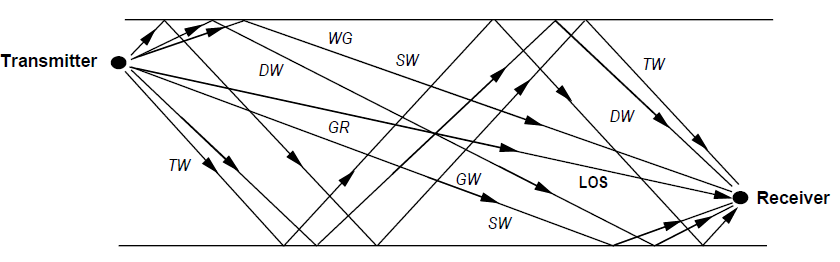
\includegraphics[width=0.8\textwidth]{fig/fig6.png}
		\caption{Overhead View of the Ten-Ray Model.}
		\label{fig:ten_ray_model}
	\end{figure}
	
	\noindent For ten-ray modellen kan det modtagne signal udtrykkes som:
	
	\[
	r_{10ray}(t) = \Re \left\{ \frac{\lambda}{4\pi} \left[ \frac{\sqrt{G_l} u(t) e^{-j2\pi l/\lambda}}{l} + \sum_{i=1}^{9} \frac{R_i \sqrt{G_{xi}} u(t - \tau_i) e^{-j2\pi x_i/\lambda}}{x_i} \right] e^{j2\pi f_c t} \right\}
	\]
	
	\noindent Her er \( x_i \) længden af stien for den i'te reflekterede stråle, \( \tau_i = \frac{(x_i - l)}{c} \) er tidsforsinkelsen mellem LOS-signalet og den i'te refleksion, og \( \sqrt{G_{xi}} \) er produktet af sender- og modtagerantennens gevinst i den i'te retning. For hver refleksionssti er koefficienten \( R_i \) enten en enkelt refleksionskoefficient (beregnet ved hjælp af ligning (2.15)) eller, hvis stien involverer flere refleksioner, produktet af refleksionskoefficienterne for hver refleksion. 
	\newline\newline
	\noindent Ligning for refleksionskoefficienten \( R \) er:
	
	\[
	R = \frac{\sin \theta - Z}{\sin \theta + Z}
	\]
	
	\noindent Hvor:
	
	\[
	Z = \begin{cases} 
		\sqrt{\epsilon_r - \cos^2\theta}/\epsilon_r & \text{for vertikal polarisering} \\
		\sqrt{\epsilon_r - \cos^2\theta} & \text{for horisontal polarisering}
	\end{cases}
	\]
	
	\noindent Her er \(\epsilon_r\) jordens eller vejens dielektriske konstant, som typisk er omkring 15.
	\newline\newline
	\noindent Den modtagne effekt kan udtrykkes som:
	
	\[
	P_r = P_t \left[ \frac{\lambda}{4\pi} \right]^2 \left| \frac{\sqrt{G_l}}{l} + \sum_{i=1}^{9} \frac{R_i \sqrt{G_{xi}} e^{-j\Delta \phi_i}}{x_i} \right|^2
	\]
	
	\noindent Hvor \( \Delta \phi_i = \frac{2\pi(x_i - l)}{\lambda} \) er faseskiftet mellem den i'te reflekterede stråle og LOS-strålen. 
	\newline\newline
	\noindent Power falloff i både ten-ray modellen og empiriske data viser, at signalstyrken falder proportionalt med \( d^{-2} \), selv ved relativt store afstande. Denne dæmpning er relativt ufølsom over for højden på senderantennen. Den kombinerede effekt af multipath-strålerne, som falder som \( d^{-2} \), og den ground-reflekterede stråle (som falder som \( d^{-4} \) i two-ray modellen) resulterer i et total power falloff med afstand, der er proportional med \( d^{-\gamma} \), hvor \( \gamma \) typisk ligger mellem to og seks.
	
	\subsubsection{Eksempel 2.6: Beregning af Modtaget Effekt for SW og DW Stier}
	
	\noindent Antag en Ten-Ray model, hvor sender- og modtagerhøjderne er \( h_t = 10 \) m og \( h_r = 2 \) m, og afstanden mellem dem er \( d = 100 \) m. Beregn den modtagne effekt for enkelt-væg (SW) og dobbelt-væg (DW) reflekterede stier ved en frekvens \( f_c = 2.4 \) GHz.	
	\newline\newline
	\noindent \textbf{Løsning:} Først beregner vi bølgelængden \( \lambda \) for frekvensen \( f_c = 2.4 \) GHz:
	
	\[
	\lambda = \frac{c}{f_c} = \frac{3 \times 10^8 \text{ m/s}}{2.4 \times 10^9 \text{ Hz}} = 0.125 \text{ m}
	\]
	
	\noindent For SW-stien (enkelt-væg) beregnes den modtagne effekt ved hjælp af:
	
	\[
	P_r \approx P_t \left[ \frac{0.125 \text{ m}}{4\pi \times 100 \text{ m}} \right]^2 \left| \frac{R_{SW} \sqrt{G_{x_{SW}}} e^{-j\Delta \phi_{SW}}}{x_{SW}} \right|^2
	\]
	
	\noindent For DW-stien (dobbelt-væg) beregnes den modtagne effekt ved at tage hensyn til dobbeltrefleksion:
	
	\[
	P_r \approx P_t \left[ \frac{0.125 \text{ m}}{4\pi \times 100 \text{ m}} \right]^2 \left| \frac{R_{DW} \sqrt{G_{x_{DW}}} e^{-j\Delta \phi_{DW}}}{x_{DW}} \right|^2
	\]
	
	\noindent Hvis vi antager, at \( x_{SW} = 120 \text{ m} \) og \( x_{DW} = 140 \text{ m} \), samt typiske værdier for refleksionskoefficienterne, kan vi beregne den samlede modtagne effekt som summen af bidragene fra begge stier.
	
	\subsubsection{Eksempel 2.7: Effekt af Dielektrisk Konstant på Modtaget Signal}
	
	\noindent Undersøg effekten af at variere den dielektriske konstant \( \epsilon_r \) fra 10 til 20 på den modtagne effekt i en Ten-Ray model ved en frekvens \( f_c = 900 \) MHz. Sender- og modtagerhøjderne er \( h_t = 15 \) m og \( h_r = 2 \) m, og afstanden \( d \) er 200 m.
	\newline\newline
	\noindent \textbf{Løsning:} Bølgelængden \( \lambda \) for frekvensen \( f_c = 900 \) MHz er:
	
	\[
	\lambda = \frac{c}{f_c} = \frac{3 \times 10^8 \text{ m/s}}{900 \times 10^6 \text{ Hz}} = 0.333 \text{ m}
	\]
	
	\noindent Reflektionskoefficienten \( R \) beregnes for hver værdi af \( \epsilon_r \) ved hjælp af ligning 2.15:
	
	\[
	R = \frac{\sin \theta - Z}{\sin \theta + Z}
	\]
	
	\noindent For \( \epsilon_r = 10 \) og \( \epsilon_r = 20 \), vi bruger værdierne til at beregne \( Z \) og derefter \( R \). Forøgelsen af \( \epsilon_r \) vil generelt reducere refleksionskoefficienten, hvilket resulterer i en lavere modtaget effekt. Den eksakte ændring i modtaget effekt kan beregnes ved at substituere de nye værdier for \( R \) i formlen for \( P_r \).
	
	\subsubsection{Eksempel 2.8: Beregning af Modtaget Effekt ved Forskellige Senderhøjder}
	For en Ten-Ray model, hvor \( h_t \) varierer mellem 5 m og 20 m, beregn den modtagne effekt ved en fast modtagerhøjde \( h_r = 3 \) m og en afstand \( d = 150 \) m. Frekvensen er \( f_c = 1.8 \) GHz.
	\newline\newline
	\noindent \textbf{Løsning:} Bølgelængden \( \lambda \) for frekvensen \( f_c = 1.8 \) GHz er:
	
	\[
	\lambda = \frac{c}{f_c} = \frac{3 \times 10^8 \text{ m/s}}{1.8 \times 10^9 \text{ Hz}} = 0.167 \text{ m}
	\]
	
	\noindent Den modtagne effekt afhænger af senderhøjden \( h_t \), da den påvirker signalets vej og de involverede refleksioner. Beregn den modtagne effekt for hver værdi af \( h_t \) ved at substituere ind i formlen for \( P_r \) og observere, hvordan effekten ændres med senderhøjden. For eksempel, hvis \( h_t \) stiger fra 5 m til 20 m, vil den modtagne effekt ændre sig markant, især på grund af ændringerne i faseskift og refleksioner.
	
	
	
	\subsection{General Ray Tracing (GRT)}
	General Ray Tracing (GRT) er en teknik, der anvendes til at forudsige signalstyrke og delay spread for ethvert bygningkonfiguration og antenneplacering. Denne metode er afhængig af en bygningdatabase, som indeholder information om højde, placering og dielektriske egenskaber af bygninger samt placeringen af transmitter- og receiverantennerne i forhold til bygningerne. Da denne information er site-specific, anvendes GRT-modellen ikke til at udlede generelle teorier om systemperformance og layout, men derimod til at forklare de grundlæggende mekanismer i urban signaludbredelse. Modellen bruges til at opnå information om delay og signalstyrke for en specifik transmitter- og receiver-konfiguration i et givet miljø.
	\newline\newline\noindent GRT-metoden bruger geometrical optics til at spore udbredelsen af Line-of-Sight (LOS) og reflekterede signal komponenter, samt signaler fra bygning diffraction og diffus scattering. Der er ingen begrænsning på antallet af multipath komponenter, der kan indregnes på en given modtager lokation. Styrken af hver komponent bestemmes eksplicit ud fra bygningernes placeringer og deres dielektriske egenskaber. I almindelighed giver LOS- og reflekterede stier de dominerende komponenter af det modtagne signal, da diffraction og scattering tab normalt er høje. Men i områder tæt på LOS og refleksionsstrålerne kan disse andre multipath-komponenter dominere.
	\subsubsection{Eksempel 1: Beregning af Signaltab gennem Bygninger}
	\noindent Antag, at vi har en bygning med en dielektrisk konstant \( \epsilon_r = 4 \). Et signal med en frekvens på 2 GHz skal passere gennem en 30 meter lang bygning. Beregn signaltabet ved hjælp af GRT-modellen.
	\newline\newline
	\noindent \textbf{Løsning:}
	\begin{enumerate}
		\item \textbf{Frekvens og Bølgelængde:} Frekvens \( f_c = 2 \) GHz. Bølgelængde \( \lambda = \frac{c}{f_c} = \frac{3 \times 10^8 \text{ m/s}}{2 \times 10^9 \text{ Hz}} = 0.15 \text{ meter} \).
		\item \textbf{Signaltab pr. meter:} Antag, at tabet pr. meter \( L_b \) er 0,5 dB/m. 
		\item \textbf{Samlet signaltab:} 
		\[
		L_{\text{total}} = L_b \times \text{distance} = 0.5 \text{ dB/m} \times 30 \text{ m} = 15 \text{ dB}
		\]
		\item \textbf{Resultat:} Det totale signaltab gennem bygningen er 15 dB.
	\end{enumerate}
	
	\subsubsection{Eksempel 2: Beregning af Refleksion fra en Bygning}
	\noindent En signalstråle reflekteres fra en glasbygning 50 meter væk fra en sender. Beregn signalstyrken ved en modtager 100 meter væk fra senderen efter refleksion.
	\newline\newline
	\noindent \textbf{Løsning:}
	\begin{enumerate}
		\item \textbf{Reflektionskoefficient:} Antag, at refleksionskoefficienten \( R \) for glas er 0.7.
		\item \textbf{Fri rums tab:}
		\[
		L_f = 20 \log_{10}\left(\frac{4\pi \times 100 \text{ m}}{\lambda}\right) \text{ dB}
		\]
		\[
		\lambda = 0.15 \text{ meter}, \quad L_f \approx 51.5 \text{ dB}
		\]
		\item \textbf{Total signaltab:}
		\[
		L_{\text{total}} = L_f + 10 \log_{10}(R) = 51.5 \text{ dB} - 1.55 \text{ dB} = 49.95 \text{ dB}
		\]
		\item \textbf{Resultat:} Den modtagne signalstyrke er reduceret med ca. 49.95 dB.
	\end{enumerate}
	
	\subsubsection{Eksempel 3: Brug af GRT til Antenneplacering}
	\noindent En mobiloperatør skal placere en antenne i en by for optimal dækning. GRT bruges til at simulere signaludbredelsen fra forskellige placeringer.
	\newline\newline
	\noindent \textbf{Løsning:}
	\begin{enumerate}
		\item \textbf{Bygningsdata:} Indlæs bygningsdata som højde, placering og dielektriske egenskaber.
		\item \textbf{Signaludbredelse:} Brug GRT til at simulere signaludbredelsen fra forskellige antenneplaceringer.
		\item \textbf{Analyse:} Sammenlign resultatet af hver placering og vælg den, der giver den bedste dækning og signalstyrke.
	\end{enumerate}
	\subsection{Knife-Edge Diffraction} Udbredelsesmodellen for LOS- og reflekterede stier blev forklaret i det forrige afsnit. Diffraction opstår, når det transmitterede signal "bøjes rundt om" et objekt på dets vej til modtageren, som vist i Figur \ref{fig:knife_edge_diffraction}. Diffraction er resultatet af mange fænomen, herunder jordens overflade, ujævnt terræn, bygninger, eller forhindringer, der blokerer LOS-path mellem transmitter og receiver.
	\newline\newline\noindent Knivkant diffraction modellen (Knife-Edge Diffraction Model) bruges ofte til at modellere diffraction, fordi den er enkel at anvende og kan levere en præcis approximation, selvom det ikke er den mest generelle model. I denne model antages det, at objektet, der forårsager diffractionen, har en kileform, hvilket er almindeligt for gadehjørner. Knivkant diffraction modellen forudsiger, at det diffrakterede signal rejser en ekstra distance \( d + d' \), hvilket resulterer i et faseskift på \( \Delta \phi = 2\pi(d + d')/\lambda \). Geometrien i Figur \ref{fig:knife_edge_diffraction} indikerer, at for \( h \) lille i forhold til \( d \) og \( d' \), skal signalet rejse en ekstra distance relativt til LOS-path på cirka:

	\[
	\Delta d = \frac{h^2 d + d'}{2 dd'}
	\]
	og det tilsvarende faseskift relativt til LOS-path er cirka:

	\[
	\Delta \phi = \frac{2\pi \Delta d}{\lambda} = \frac{\pi}{2} v^2
	\]
	hvor
	
	\[
	v = h \frac{\sqrt{2(d+d')}}{\lambda \cdot d \cdot d'}
	\]
	\noindent Dette kaldes Fresnel-Kirchhoff diffraction parameteren. De tilhørende tab, kaldet knife-edge diffraction loss, er en funktion af \( v \). Approximationer for knife-edge diffraction loss i dB relativt til LOS-path loss er givet af:

	\[
	L(v) \text{ dB} = \left\{
	\begin{array}{ll}
		20 \log_{10}[0.5 - 0.62v] & -0.8 \leq v < 0 \\
		20 \log_{10}[0.5e^{-0.95v}] & 0 \leq v < 1 \\
		20 \log_{10}[0.4 - \sqrt{0.1184 - (0.38 - 0.1v)^2}] & 1 \leq v < 2.4 \\
		20 \log_{10}[0.225/v] & v \geq 2.4
	\end{array}
	\right.
	\]
	\noindent Knife-edge diffraction modellen giver følgende formel for det modtagne diffrakterede signal:

	\[
	r(t) = \Re \left\{ L(v) \sqrt{G_d} u(t - \tau) e^{-j2\pi(d+d')/\lambda} e^{j2\pi f_c t} \right\}
	\]
	\noindent hvor \( \sqrt{G_d} \) er antenneforstærkningen og \( \tau = \Delta d / c \) er forsinkelsen forbundet med det diffrakterede signal relativt til LOS-path.
	\begin{figure}[h]
		\centering
		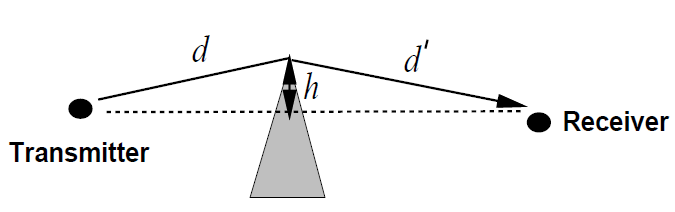
\includegraphics[width=0.8\textwidth]{fig/fig7.png}
		\caption{Knife-Edge Diffraction.}
		\label{fig:knife_edge_diffraction}
	\end{figure}
	\subsubsection{Eksempel 4: Beregning af Faseskift ved Knife-Edge Diffraction}
	\noindent Et signal diffrakteres omkring et hjørne med en højde \( h = 10 \) meter. Afstanden til modtageren er \( d = 100 \) meter, og til den anden side af hjørnet \( d' = 50 \) meter. Frekvensen er 2.4 GHz. Beregn faseskiftet \( \Delta \phi \).
	\newline\newline
	\noindent \textbf{Løsning:}
	\begin{enumerate}
		\item \textbf{Beregning af bølgelængde:} 
		\[
		\lambda = \frac{c}{f_c} = \frac{3 \times 10^8}{2.4 \times 10^9} = 0.125 \text{ meter}
		\]
		\item \textbf{Beregn \( v \):}
		\[
		v = h \frac{\sqrt{2(d+d')}}{\lambda \cdot d \cdot d'} = 10 \cdot \frac{\sqrt{2 \cdot (100 + 50)}}{0.125 \cdot 100 \cdot 50} = 0.8
		\]
		\item \textbf{Beregn faseskift \( \Delta \phi \):}
		\[
		\Delta \phi = \frac{\pi}{2}v^2 = \frac{\pi}{2}(0.8)^2 = 1.005 \text{ rad}
		\]
		\item \textbf{Resultat:} Faseskiftet er ca. 1.005 radianer.
	\end{enumerate}
	
	\subsubsection{Eksempel 5: Beregning af Diffraction Tab}
	\noindent Antag, at \( v = 1.5 \) for en given knife-edge diffraction. Beregn diffraction tabet \( L(v) \) i dB.
	\newline\newline
	\noindent \textbf{Løsning:}
	\begin{enumerate}
		\item \textbf{Beregn diffraction tabet:}
		\[
		L(v) \text{ dB} = 20 \log_{10}[0.4 - \sqrt{0.1184 - (0.38 - 0.1 \cdot 1.5)^2}]
		\]
		\item \textbf{Resultat:} Diffraction tabet er ca. -12 dB.
	\end{enumerate}
	
	\subsubsection{Eksempel 6: Modtaget Signalstyrke efter Diffraction}
	\noindent Et signal med en styrke på 0 dBm diffrakteres omkring et objekt med \( v = 2 \). Beregn den modtagne signalstyrke.
	\newline\newline
	\noindent \textbf{Løsning:}
	\begin{enumerate}
		\item \textbf{Beregn diffraction tabet:} 
		\[
		L(v) \text{ dB} = 20 \log_{10}[0.225/v] = 20 \log_{10}[0.225/2] = -20 \text{ dB}
		\]
		\item \textbf{Modtaget signalstyrke:} 
		\[
		P_r = 0 \text{ dBm} - 20 \text{ dB} = -20 \text{ dBm}
		\]
		\item \textbf{Resultat:} Den modtagne signalstyrke er -20 dBm.
	\end{enumerate}
	
	\subsection{Scattering}
	\noindent Foruden diffrakterede stråler kan der også være stråler, der er diffrakterede flere gange eller stråler, der både er reflekterede og diffrakterede. Modeller findes for at inkludere alle mulige permutationer af refleksion og diffraction, men attenuationen af de tilsvarende signal komponenter er generelt så stor, at disse komponenter er negligibelt i forhold til støj. Diffraction modeller kan også specialiseres til et givet miljø. For eksempel blev en model for diffraction fra bygninger og tage i cellular systems udviklet af Walfisch og Bertoni. 
	\newline\newline\noindent En scattered stråle, vist i Figur \ref{fig:scattering}, har et path loss proportionalt med produktet af \( s \) og \( s' \). Denne multiplicative afhængighed skyldes det ekstra spredningstab, som strålen oplever efter spredning. Det modtagne signal på grund af en scattered stråle er givet af den bistatiske radar ligning:

	\[
	r(t) = \Re \left\{ u(t - \tau) \frac{\lambda \sqrt{G_s} \sigma e^{-j2\pi(s+s')/\lambda}}{(4\pi)^{3/2}ss'} e^{j2\pi f_c t} \right\}
	\]
	\noindent hvor \( \tau = (s + s' - l)/c \) er forsinkelsen forbundet med den spredte stråle, \( \sigma \) er radar cross section for scatteren, og \( G_s \) er antenneforstærkning. Denne model antager, at signalet udbreder sig fra transmitter til scatterer baseret på free space propagation og derefter reemitteres af scatteren med transmit power \( \sigma \) til at estimere den modtagne effekt ved scattereren.
	
	\begin{figure}[!h]
		\centering
		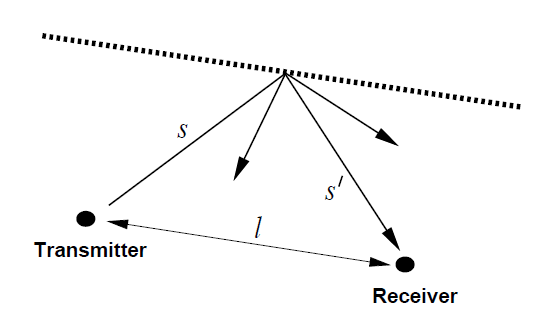
\includegraphics[width=0.6\textwidth]{fig/fig8.png}
		\caption{Scattering.}
		\label{fig:scattering}
	\end{figure}

	\subsubsection{Eksempel 7: Beregning af Spredt Signalstyrke}
	\noindent Et signal spredes af en lille metalgenstand med en radar cross section \( \sigma = 0.1 \) kvadratmeter. Afstanden mellem senderen og objektet er 50 meter, og mellem objektet og modtageren er 70 meter. Frekvensen er 1.8 GHz. Beregn den modtagne signalstyrke.
	\noindent \textbf{Løsning:}
	\begin{enumerate}
		\item \textbf{Beregning af bølgelængde:} 
		\[
		\lambda = \frac{c}{f_c} = \frac{3 \times 10^8}{1.8 \times 10^9} \approx 0.167 \text{ meter}
		\]
		\item \textbf{Beregn spredt signalstyrke:}
		\[
		P_r = P_t \cdot \frac{\lambda \sqrt{G_s} \sigma}{(4\pi)^{3/2}ss'} 
		\]
		\[
		s = 50 \text{ meter}, \quad s' = 70 \text{ meter}, \quad G_s = 1, \quad \sigma = 0.1
		\]
		\[
		P_r = P_t \cdot \frac{0.167 \times 0.1}{(4\pi)^{3/2} \times 50 \times 70} \approx P_t \cdot 1.59 \times 10^{-8}
		\]
		\item \textbf{Resultat:} Den modtagne signalstyrke vil være meget lav, ca. \( P_t \times 1.59 \times 10^{-8} \).
	\end{enumerate}
	
	\subsubsection{Eksempel 8: Effekt af Antennens Gain på Spredt Signal}
	\noindent Hvis antennen har en gain \( G_s = 3 \) ved en frekvens på 2.4 GHz, og signalet spredes af et objekt 100 meter væk, beregn effekten af denne gain på den modtagne signalstyrke.
	
	\noindent \textbf{Løsning:}
	\begin{enumerate}
		\item \textbf{Beregning af spredt signalstyrke:} 
		\[
		P_r = P_t \cdot \frac{\lambda \sqrt{G_s} \sigma}{(4\pi)^{3/2}ss'}
		\]
		\[
		G_s = 3, \quad s = 100 \text{ meter}, \quad s' = 100 \text{ meter}, \quad \sigma = 0.1
		\]
		\[
		P_r = P_t \cdot \frac{0.125 \times \sqrt{3} \times 0.1}{(4\pi)^{3/2} \times 100 \times 100}
		\]
		\item \textbf{Resultat:} Den modtagne signalstyrke stiger i forhold til \( G_s = 1 \).
	\end{enumerate}
	
	\subsubsection{Eksempel 9: Beregning af Spredningstab}
	\noindent Beregn spredningstab, når et signal med \( P_t = 10 \) dBm reflekteres og spredes af et objekt 70 meter væk fra både sender og modtager.
	
	\noindent \textbf{Løsning:}
	\begin{enumerate}
		\item \textbf{Beregning af bølgelængde:}
		\[
		\lambda = 0.167 \text{ meter}, \quad s = s' = 70 \text{ meter}, \quad \sigma = 0.05
		\]
		\item \textbf{Spredt signalstyrke:}
		\[
		P_r = 10 \text{ dBm} + 10 \log_{10}\left( \frac{0.167 \times 0.05}{(4\pi)^{3/2} \times 70 \times 70} \right)
		\]
		\item \textbf{Resultat:} 
		\[
		P_r \approx -60 \text{ dBm}
		\]
	\end{enumerate}

	\subsection{Local Mean Received Power}
	The path loss beregnet fra alle ray tracing modeller er forbundet med en fast transmitter og receiver lokation. Derudover kan ray tracing bruges til at beregne den lokale gennemsnitlige
	modtagne effekt \( P_r \) i nærheden af en given receiver lokation ved at tilføje den kvadrerede størrelse af alle de modtagne stråler. Dette har effekten af at udglatte lokale spatial variationer på grund af faseændringer rundt omkring en given lokation. Local mean received power er en god indikator for link quality og bruges ofte i cellular systems til power control og handoff.
	
	\subsection{Local Mean Received Power} Det path loss, som beregnes fra alle ray tracing-modeller, er knyttet til en fast position af både sender og modtager. Når man arbejder med trådløse signaler, er det dog også vigtigt at
	forstå, hvordan den modtagne effekt varierer i et lokalt område omkring modtageren. Dette kan gøres ved at beregne den \textit{local mean received power} \( \overline{P_r} \).
	\newline\newline
	\textit{Local mean received power} er den gennemsnitlige værdi af den modtagne effekt i et lille område omkring modtageren. For at beregne denne størrelse, tager man højde for alle de forskellige signalveje (rays), der når frem til modtageren. Hver af disse signaler kan have en forskellig amplitude og fase, hvilket betyder, at når man summerer bidragene fra alle signalerne, skal man først kvadrere hver signals amplitude, inden man summerer dem. Denne proces udjævner lokale rumlige variationer, som skyldes faseændringer omkring den specifikke position.
	\newline\newline
	Den \textit{local mean received power} \( \overline{P_r} \) er en god indikator for kvaliteten af en trådløs forbindelse og anvendes ofte i cellulære systemer til funktioner som power control og handoff.
	
	\section{Empiriske Path Loss Modeller}
	Empiriske path loss modeller bruges til at forudsige signalstyrke i komplekse udbredelsesmiljøer, hvor simple modeller som free-space path loss eller ray tracing ikke er tilstrækkelige. Disse modeller er baseret på faktiske målinger af signaludbredelse i specifikke miljøer, såsom store byområder (\textit{urban macrocells}), mindre byområder (\textit{urban microcells}) og indendørs omgivelser. Modellerne anvender typisk data fra bestemte geografiske områder eller bygningstyper og giver os mulighed for at vurdere signalstyrken på forskellige afstande og frekvenser.
	
	\subsection{The Okumura Model}
	Okumura-modellen er en af de mest anvendte modeller til signalforudsigelse i store byområder. Modellen er gældende over afstande fra 1 til 100 km og frekvensområder fra 150 til 1500 MHz. Den er baseret på omfattende målinger af signaludbredelse fra basestationer til mobile enheder i Tokyo, Japan. Modellen estimerer den mediane attenuation i forhold til free space udbredelse. Formlen for path loss ved en afstand \(d\) er:
	
	\[
	P_L(d) = L(f_c, d) + A_{\text{mu}}(f_c, d) - G(h_t) - G(h_r) - G_{\text{AREA}}
	\]
	
	Her er:
	\begin{itemize}
		\item \( L(f_c, d) \): free space path loss ved afstand \(d\) og frekvens \(f_c\),
		\item \( A_{\text{mu}}(f_c, d) \): den mediane attenuation,
		\item \( G(h_t) \): gevinst fra senderantennens højde, beregnet som:
		\[
		G(h_t) = 20\log_{10}\left(\frac{h_t}{200}\right), \quad 30m < h_t < 1000m
		\]
		\item \( G(h_r) \): gevinst fra modtagerantennens højde, beregnet som:
		\[
		G(h_r) = \left\{
		\begin{array}{ll}
			10\log_{10}\left(\frac{h_r}{3}\right), & h_r \leq 3m \\
			20\log_{10}\left(\frac{h_r}{3}\right), & 3m < h_r \leq 10m 
		\end{array}
		\right.
		\]
		\item \( G_{\text{AREA}} \): gevinst afhængig af områdets karakteristika.
	\end{itemize}
	
	\subsection{The Hata Model}
	Hata-modellen er en videreudvikling af Okumura-modellen og bruges til at forenkle beregningen af path loss med en lukket formel. Denne model dækker stort set samme frekvensområde som Okumura-modellen og bruges især i byområder. Formlen for path loss i byområder er:
	
	\[
	P_L(d) = 69.55 + 26.16 \log_{10}(f_c) - 13.82 \log_{10}(h_t) - a(h_r) + \left( 44.9 - 6.55 \log_{10}(h_t) \right) \log_{10}(d)
	\]
	
	Her er \( a(h_r) \) en korrektion for modtagerantennens højde afhængigt af størrelsen af byområdet, beregnet som:
	
	\[
	a(h_r) = \left\{
	\begin{array}{ll}
		(1.1 \log_{10}(f_c) - 0.7)h_r - (1.56 \log_{10}(f_c) - 0.8) \text{ dB}, & \text{for små til mellemstore byer,} \\
		3.2(\log_{10}(11.75h_r))^2 - 4.97 \text{ dB}, & \text{for større byer,} \\
	\end{array}
	\right.
	\]
	
	\subsection{COST 231 Udvidelse til Hata Modellen}
	COST 231 er en udvidelse af Hata-modellen, som dækker højere frekvenser (op til 2 GHz) og bruges i byområder med mellemstore byer og forstæder. Formlen for path loss er:
	
	\[
	P_L(d) = 46.3 + 33.9 \log_{10}(f_c) - 13.82 \log_{10}(h_t) - a(h_r) + \left( 44.9 - 6.55 \log_{10}(h_t) \right) \log_{10}(d) + C_M
	\]
	
	Hvor \( C_M \) er en konstant på 0 dB for byområder og 3 dB for forstæder.
	
	\subsection{Piecewise Linear (Multi-Slope) Model}
	
	En almindelig empirisk metode til modellering af \textit{path loss} i udendørs \textit{microcells} og indendørs kanaler er \textit{piecewise linear} modellen, som illustrerer dB-tab som funktion af log-afstanden. Denne tilgang er illustreret i Figur \ref{fig:piecewise_linear_model}, hvor punkterne repræsenterer hypotetiske empiriske målinger, og den stykvis lineære model repræsenterer en approximation til disse målinger. En \textit{piecewise linear} model med \(N\) segmenter skal specificere \(N-1\) brudpunkter \(d_1, d_2, \ldots, d_{N-1}\) og hældningerne svarende til hvert segment \(s_1, s_2, \ldots, s_N\). Forskellige metoder kan bruges til at bestemme antallet og placeringen af brudpunkter i modellen. Når disse er fastlagt, kan hældningerne svarende til hvert segment opnås ved lineær regression.
	
	\begin{figure}[h]
		\centering
		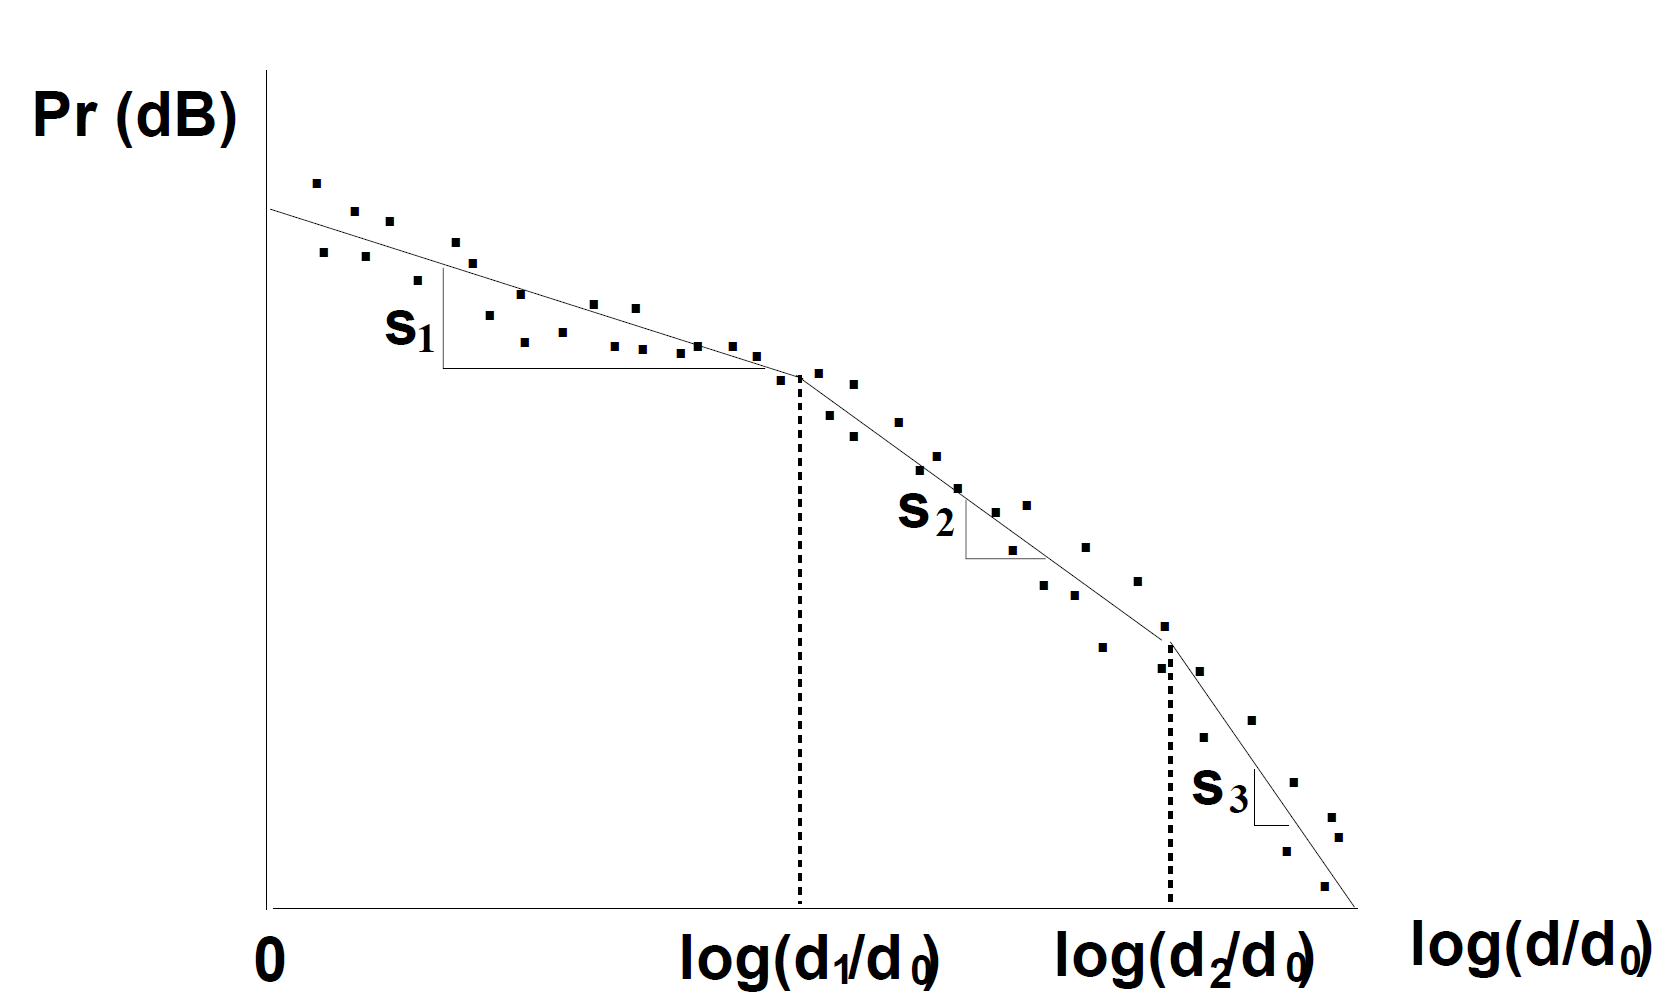
\includegraphics[width=0.8\textwidth]{fig/fig9.png}
		\caption{Piecewise Linear Model for Path Loss.}
		\label{fig:piecewise_linear_model}
	\end{figure}
	
	En specialtilfælde af den stykvis lineære model er \textit{dual-slope} modellen. \textit{Dual-slope} modellen er karakteriseret ved en konstant \textit{path loss factor} \(K\) og en \textit{path loss} eksponent \( \gamma_1 \) over en referenceafstand \( d_0 \) op til en kritisk afstand \( d_c \), hvorefter signalet falder med \textit{path loss} eksponenten \( \gamma_2 \):
	
	\[
	P_r(d) \, \text{dB} = 
	\begin{cases} 
		P_t + K - 10 \gamma_1 \log_{10}(d/d_0) & \text{for } d_0 \leq d \leq d_c \\
		P_t + K - 10 \gamma_1 \log_{10}(d_c/d_0) - 10 \gamma_2 \log_{10}(d/d_c) & \text{for } d > d_c 
	\end{cases}
	\]
	
	Her er \(P_t\) transmitterens effekt, \(P_r(d)\) den modtagne effekt som funktion af afstanden, og \(\gamma_1\) samt \(\gamma_2\) er \textit{path loss} eksponenter, der typisk opnås via regression af empiriske data.
	\newline\newline
	De multiple ligninger i \textit{dual-slope} modellen kan samles i følgende \textit{dual-slope} approximation:
	
	\[
	P_r = \frac{P_t K}{L(d)}
	\]
	
	hvor
	
	\[
	L(d) \triangleq \left(\frac{d}{d_0}\right)^{\gamma_1} \sqrt{1 + \left(\frac{d}{d_c}\right)^{(\gamma_1 - \gamma_2)q}}
	\]
	
	I dette udtryk er \(q\) en parameter, der bestemmer smoothness af \textit{path loss} ved overgangsområdet tæt på brudpunktet \(d_c\). Denne model kan udvides til mere end to regioner, hvis det er nødvendigt.
	\newline\newline
	Denne stykvis lineære model giver en fleksibel metode til at modellere \textit{path loss} over et bredt spektrum af afstande og anvendes ofte i både udendørs og indendørs kanaler.
	
	
	\subsection{Indendørs Attenuation Faktorer}
	Indendørs path loss modeller er essentielle for at forudsige signalstyrke inde i bygninger, hvor signalet møder forskellige hindringer som vægge, gulve og møbler. Tabellen nedenfor viser typiske attenuationer for forskellige materialer:
	
	\begin{table}[h]
		\centering
		\begin{tabular}{|l|c|}
			\hline
			\textbf{Materiale} & \textbf{Attenuation (dB)} \\
			\hline
			Tøj & 1.4 \\
			Dobbelt gipsvæg & 3.4 \\
			Foilisolering & 3.9 \\
			Betonvæg & 13 \\
			Aluminiumskonstruktion & 20.4 \\
			Alt Metal & 26 \\
			\hline
		\end{tabular}
		\caption{Typiske partitionstab for indendørs omgivelser.}
	\end{table}
	
	Disse data anvendes i formlen:
	
	\[
	P_r \, \text{dBm} = P_t \, \text{dBm} - P_L(d) - \sum_{i=1}^{N_f} FAF_i - \sum_{i=1}^{N_p} PAF_i
	\]
	
	Hvor:
	\begin{itemize}
		\item \( FAF_i \) er floor attenuation factor for den \( i \)te etage,
		\item \( PAF_i \) er partition attenuation factor for den \( i \)te skillevæg.
	\end{itemize}
	
	\noindent 
	Disse faktorer er essentielle for at beregne præcis signalstyrke inde i bygninger, hvor hver etage eller væg bidrager til det samlede path loss.
	
	
	\section{Simplified Path Loss Model}
	Når vi arbejder med trådløs kommunikation, er det vigtigt at kunne forudsige, hvordan signalstyrken ændrer sig, når afstanden mellem sender og modtager øges. Dette kaldes ofte for \textit{path loss}, og det beskriver, hvor meget af signalets styrke der går tabt på vej til modtageren.
	\newline\newline
	Der findes mange modeller, der kan bruges til at forudsige \textit{path loss}, men ofte kan en simpel model være tilstrækkelig til at give os en god forståelse af, hvad der sker. En af disse enkle modeller beskriver forholdet mellem modtagen effekt \( P_r \) og senderens effekt \( P_t \) som:
	
	\[
	P_r = P_t K \left[\frac{d_0}{d}\right]^\gamma
	\]
	
	\noindent hvor:
	
	- \( P_r \) er den modtagne effekt ved modtageren.
	- \( P_t \) er den effekt, der sendes fra senderen.
	- \( K \) er en konstant, som afhænger af antennens egenskaber og det gennemsnitlige signaltab i kanalen.
	- \( d_0 \) er en referenceafstand, typisk valgt i nærheden af senderen, hvor signalet stadig er stærkt.
	- \( d \) er afstanden mellem sender og modtager.
	- \( \gamma \) er \textit{path loss} eksponenten, som beskriver, hvor hurtigt signalet mister styrke over afstand.
	\newline\newline
	Denne model viser, at signalet bliver svagere, jo længere væk modtageren er fra senderen. Konstanten \( K \) kan beregnes ved hjælp af følgende formel, hvor \( \lambda \) er signalets bølgelængde:
	
	\[
	K \, \text{dB} = 20 \log_{10} \left(\frac{\lambda}{4\pi d_0}\right)
	\]
	
	\noindent Dette udtryk bruger vi, når vi ønsker at finde ud af, hvor meget signalstyrken falder ved en bestemt afstand \( d \) fra senderen.
	
	\subsection{Eksempel 1: Beregning af Path Loss Eksponent og Modtaget Effekt}
	\textbf{Problem:} Vi har et sæt empiriske målinger af forholdet mellem modtagen og sendt effekt \( P_r/P_t \) ved 900 MHz, som vist i tabellen nedenfor. Vi skal finde den \textit{path loss} eksponent \( \gamma \), der minimerer middelkvadratfejlen (MSE) mellem den simplificerede model (ligning 2.40) og de empiriske dB målinger, idet vi antager, at \( d_0 = 1 \) meter og \( K \) er bestemt ud fra \textit{free space path loss} formlen ved denne afstand. Dernæst skal vi beregne den modtagne effekt ved 150 meter for den simplificerede \textit{path loss} model med denne \( \gamma \) og en sendeeffekt på 1 mW (0 dBm).
	
	\begin{table}[h]
		\centering
		\begin{tabular}{|c|c|}
			\hline
			Afstand fra Transmitter (m) & \( M = P_r/P_t \) \\
			\hline
			10 m & -70 dB \\
			20 m & -75 dB \\
			50 m & -90 dB \\
			100 m & -110 dB \\
			300 m & -125 dB \\
			\hline
		\end{tabular}
		\caption{Path Loss målinger}
	\end{table}
	
	\noindent\textbf{Løsning:} Vi opstiller først MSE-fejludtrykket for dB målingerne som:
	
	\[
	F(\gamma) = \sum_{i=1}^{5} \left[ M_{\text{measured}}(d_i) - M_{\text{model}}(d_i) \right]^2
	\]
	
	hvor \( M_{\text{measured}}(d_i) \) er path loss målingen fra tabel 2.3 ved afstand \( d_i \), og \( M_{\text{model}}(d_i) \) er path loss baseret på (2.40) ved \( d_i \). Ved brug af formlen for \textit{free space path loss}, \( K = 20 \log_{10}(0.3333/(4\pi)) = -31.54 \) dB, får vi:
	
	\[
	F(\gamma) = (-70 + 31.54 + 10\gamma \log_{10}(10))^2 + (-75 + 31.54 + 13.01\gamma)^2 + (-90 + 31.54 + 16.99\gamma)^2 
	\]
	\[
	+ (-110 + 31.54 + 20\gamma)^2 + (-125 + 31.54 + 24.77\gamma)^2 
	\]
	\[
	F(\gamma) = 21676.3 - 11654.9\gamma + 1571.47\gamma^2
	\]
	
	\noindent Ved at differentiere \( F(\gamma) \) med hensyn til \( \gamma \) og sætte det lig nul, får vi:
	
	\[
	\frac{\partial F(\gamma)}{\partial \gamma} = -11654.9 + 3142.94\gamma = 0 \Rightarrow \gamma = 3.71
	\]
	
	For at finde den modtagne effekt ved 150 meter under den simplificerede \textit{path loss} model med \( K = -31.54 \) dB, \( \gamma = 3.71 \), og \( P_t = 0 \) dBm, har vi:
	
	\[
	P_r = P_t + K - 10\gamma \log_{10}(d/d_0) = 0 - 31.54 - 10 \times 3.71 \log_{10}(150/1) 
	\]
	\[
	P_r = -31.54 - 10 \times 3.71 \times 2.176 = -31.54 - 80.58 = -112.12 \text{ dBm}
	\]
	
	\noindent Denne afvigelse fra den simplificerede \textit{path loss} model kan tilskrives \textit{shadow fading}, som er beskrevet i Sektion 2.7.
	
	\subsection{Eksempel 2: Beregning af Modtaget Effekt ved 200 meter}
	\textbf{Problem:} Vi ønsker at beregne den modtagne effekt ved en afstand på 200 meter fra senderen, hvor den sendte effekt \( P_t \) er 1 mW (0 dBm), og \( \gamma = 3.71 \) er bestemt fra det foregående eksempel.
	\newline\newline\noindent
	\textbf{Løsning:} Vi anvender den samme formling som tidligere:
	
	\[
	P_r = P_t + K - 10\gamma \log_{10}(d/d_0)
	\]
	
	\[
	P_r = 0 \text{ dBm} - 31.54 - 10 \times 3.71 \log_{10}(200/1)
	\]
	
	\[
	P_r = -31.54 - 10 \times 3.71 \times 2.301 = -31.54 - 85.41 = -116.95 \text{ dBm}
	\]
	
	\textbf{Resultat:} Den modtagne effekt ved 200 meters afstand er cirka -116.95 dBm.
	
	\subsection{Eksempel 3: Effekt af \textit{Shadow Fading}}
	
	\textbf{Problem:} Antag, at vi har en situation, hvor \textit{shadow fading} introducerer en ekstra dæmpning på 10 dB ved en afstand på 100 meter. Beregn den samlede modtagne effekt under disse forhold.
	\newline\newline\noindent
	\textbf{Løsning:} Først beregner vi den modtagne effekt uden \textit{shadow fading}:
	
	\[
	P_r = 0 \text{ dBm} - 31.54 - 10 \times 3.71 \log_{10}(100/1)
	\]
	
	\[
	P_r = -31.54 - 10 \times 3.71 \times 2 = -31.54 - 74.2 = -105.74 \text{ dBm}
	\]
	
	Dernæst tager vi \textit{shadow fading} i betragtning:
	
	\[
	P_r = -105.74 \text{ dBm} - 10 \text{ dB} = -115.74 \text{ dBm}
	\]
	\noindent\textbf{Resultat:} Den samlede modtagne effekt ved 100 meter afstand, inklusive \textit{shadow fading}, er cirka -115.74 dBm.
	
	
	\subsection{Opsummering}
	
	Disse eksempler viser, hvordan vi kan bruge den simplificerede \textit{path loss} model til at beregne signalstyrken ved forskellige afstande i forskellige miljøer. Modellen gør det muligt at forudsige, hvor meget signalstyrken vil falde, og dermed hjælpe med at designe mere effektive trådløse netværk.
	
	
	\section{Shadow Fading og Log-Normal Skjulte Variabler}
	
	I trådløs kommunikation oplever signaler ofte variationer i modtaget effekt på grund af forhindringer som bygninger, træer eller andre objekter, der blokerer signalets vej. Denne tilfældige variation i signalstyrken kaldes \textit{shadow fading} eller log-normal fading, og det kan føre til væsentlige udsving i signalkvaliteten. For at modellere denne variation benyttes ofte en statistisk model kendt som log-normal fading model, som beskriver signalets dæmpning over afstand i en given kanal.
	
	\subsection{Log-Normal Skjulte Variabler}
	
	I log-normal fading-modellen antages det, at forholdet mellem den transmitterede effekt \( P_t \) og den modtagne effekt \( P_r \) er en tilfældig variabel \( \psi = \frac{P_t}{P_r} \), som er log-normalt fordelt. Dette betyder, at \( \log_{10}(\psi) \) er normalfordelt, hvilket kan udtrykkes som:
	
	\[
	p(\psi) = \frac{\xi}{\sqrt{2\pi\sigma_{\psi\text{dB}}^2}} \exp \left[ -\frac{(\log_{10}\psi - \mu_{\psi\text{dB}})^2}{2\sigma_{\psi\text{dB}}^2} \right], \quad \psi > 0
	\]
	
	hvor \( \xi = \frac{10}{\ln 10} \), \( \mu_{\psi\text{dB}} \) er middelværdien af \( \log_{10}(\psi) \) i dB, og \( \sigma_{\psi\text{dB}} \) er standardafvigelsen af \( \log_{10}(\psi) \) i dB.
	
	\subsection{Gennemsnit og Varians af \( \log_{10}(\psi) \)}
	
	Det er vigtigt at bemærke, at hvis \( \psi \) er log-normal, vil gennemsnittet og standardafvigelsen af \( \log_{10}(\psi) \) også være log-normale. Det betyder, at både modtagerens signal-til-støj-forhold (SNR) og modtagerens effekt vil være log-normale størrelser. Middelværdien \( \mu_\psi \) og standardafvigelsen \( \sigma_\psi \) for den modtagne effekt i dB kan findes ved:
	
	\[
	\mu_\psi = \mathbb{E}[\psi] = \exp \left[ \mu_{\psi\text{dB}} + \frac{\sigma_{\psi\text{dB}}^2}{2\xi^2} \right]
	\]
	
	Og konverteringen fra lineær middelværdi til log-middelværdi er givet ved:
	
	\[
	10 \log_{10} \mu_\psi = \mu_{\psi\text{dB}} + \frac{\sigma_{\psi\text{dB}}^2}{2\xi^2}
	\]
	
	\subsection{Shadow Fading Modellering}
	
	Modelleringen af shadow fading indebærer at finde middelværdi og varians af \( \psi \) for at forstå, hvordan modtaget effekt varierer i forskellige miljøer. Typisk er standardafvigelsen \( \sigma_{\psi\text{dB}} \) i området fra 4 til 13 dB, afhængigt af miljøet. For eksempel vil urban macrocells have en højere standardafvigelse på grund af flere forhindringer end åbne områder.
	
	En vigtig del af denne model er at forudsige signalstyrken \( s(d) \) som en funktion af afstanden \( d \) fra senderen:
	
	\[
	s(d) = e^{-\alpha d}
	\]
	
	hvor \( \alpha \) er en dæmpningskonstant, der afhænger af objekternes materialer og dielektriske egenskaber. Når signalet passerer gennem flere objekter, vil den samlede dæmpning \( s(d) \) være:
	
	\[
	s(d_t) = e^{-\alpha \sum d_i} = e^{-\alpha d_t}
	\]
	
	hvor \( d_t \) er summen af dybderne af alle objekterne mellem senderen og modtageren.
	
	\subsection{Eksempler}
	
	\subsubsection{Eksempel 2.4: Beregning af Shadow Fading Varians}
	
	Givet en række målinger af \( \frac{P_r}{P_t} \) fra et indendørs system ved 900 MHz, beregn variansen \( \sigma_{\psi\text{dB}}^2 \) for shadow fading over en given afstand.
	
	\begin{enumerate}
		\item \textbf{Dataanalyse}: Vi tager fem målepunkter fra tabel 2.3, der giver os \( M_{\text{measured}}(d_i) \) og \( M_{\text{model}}(d_i) \).
		\item \textbf{Fejlberegning}: Vi beregner fejlens kvadratrod ved hver afstand ved at sammenligne den målte effekt med den beregnede model.
		\item \textbf{Variansberegning}:
		\[
		\sigma_{\psi\text{dB}}^2 = \frac{1}{5} \sum_{i=1}^{5} \left[ M_{\text{measured}}(d_i) - M_{\text{model}}(d_i) \right]^2
		\]
		\item \textbf{Resultat}: Vi finder \( \sigma_{\psi\text{dB}} = 3.65 \) dB, hvilket er standardafvigelsen for shadow fading i dette miljø.
	\end{enumerate}
	
	\subsubsection{Eksempel 2.5: Beregning af Skjulte Variabler i Et Byområde}
	
	Antag en frekvens på 2 GHz i et byområde med høje bygninger. Beregn den gennemsnitlige effekt \( \mu_{\psi\text{dB}} \) for modtageren placeret 100 meter væk fra senderen.
	
	\begin{enumerate}
		\item \textbf{Middelværdi i dB}:
		\[
		\mu_{\psi\text{dB}} = \exp \left[ \mu_{\psi\text{dB}} + \frac{\sigma_{\psi\text{dB}}^2}{2\xi^2} \right]
		\]
		\item \textbf{Standardafvigelse}: Antag \( \sigma_{\psi\text{dB}} = 8 \) dB, og brug de tidligere angivne data til at beregne den gennemsnitlige modtagne effekt.
		\item \textbf{Resultat}: Den modtagne effekt er reduceret betydeligt på grund af shadow fading, især i byområder.
	\end{enumerate}
	
	\subsubsection{Eksempel 2.6: Anvendelse af Shadow Fading i Et Mikrocellulært Miljø}
	
	Beregning af signalstyrken for et mikrocellesystem ved 2 GHz, hvor modtageren er placeret 50 meter væk fra senderen, og der er flere forhindringer som træer og bygninger.
	
	\begin{enumerate}
		\item \textbf{Dæmpningskonstant}:
		\[
		\alpha = \frac{\sigma_{\psi\text{dB}}}{\sqrt{2}}
		\]
		\item \textbf{Beregn signalstyrken}:
		\[
		s(d) = e^{-\alpha d}
		\]
		\item \textbf{Resultat}: Variationen i signalstyrken afhænger af antallet og størrelsen af forhindringerne mellem senderen og modtageren.
	\end{enumerate}
	
	Disse eksempler hjælper med at forstå, hvordan shadow fading påvirker signaludbredelsen i forskellige miljøer og hvordan det kan modelleres for at optimere trådløse kommunikationssystemer.
	
	\section{Combined Path Loss and Shadowing}
	Modeller for path loss og shadowing kan kombineres for at fange både effekten af signalstyrketab over afstand samt tilfældig attenuation, der skyldes shadowing. I denne kombinerede model bliver det gennemsnitlige dB path loss karakteriseret af path loss-modellen, mens shadow fading med en middelværdi på 0 dB skaber variationer omkring dette path loss, som illustreret af kurven i figur 2.1. Specifikt plotter denne kurve kombinationen af den forenklede path loss-model (ligning 2.39) og den log-normal shadowing tilfældige proces defineret af ligningerne (2.46) og (2.50). For denne kombinerede model er forholdet mellem modtaget og transmitteret effekt i dB givet ved:
	
	\[
	\frac{P_r}{P_t} \text{(dB)} = 10 \log_{10} K - 10 \gamma \log_{10}\left(\frac{d}{d_0}\right) - \psi_{\text{dB}},
	\]
	\noindent hvor \( \psi_{\text{dB}} \) er en Gauss-fordelt tilfældig variabel med middelværdien nul og variansen \( \sigma^2_{\psi_{\text{dB}}} \). I ligning (2.51) og som vist i figur 2.1, falder path loss lineært i forhold til \( \log_{10}(d) \) med en hældning på \( 10 \gamma \) dB per dekade, hvor \( \gamma \) er path loss eksponenten. Variationer som følge af shadowing ændrer sig hurtigere, afhængig af decorrelation distance \( X_c \).
	
	De foregående eksempler 2.3 og 2.4 illustrerer den kombinerede model for path loss og log-normal shadowing baseret på målingerne i tabel 2.3, hvor path loss følger den forenklede model med \( K = -31.54 \) dB og path loss eksponenten \( \gamma = 3.71 \), mens shadowing følger log-normal modellen med middelværdi givet af path loss modellen og standardafvigelsen \( \sigma_{\psi_{\text{dB}}} = 3.65 \) dB.
	
	\subsection{Statistisk Baggrund for Shadowing}
	Shadowing refererer til de tilfældige udsving i signalstyrken, som skyldes blokeringer eller forhindringer i signalets vej, som kan være forårsaget af bygninger, træer eller andre objekter. Disse udsving modelleres ofte som en log-normal fordeling, hvor \( \psi_{\text{dB}} \) beskriver forskellen mellem den forventede signalstyrke og den faktiske målte styrke.
	
	Den log-normale fordeling er kendetegnet ved, at hvis \( \psi \) i sig selv varierer over en bred vifte, så vil \( \log_{10}(\psi) \) være normalfordelt. Dette gør det muligt at bruge standardstatistiske metoder til at analysere dataene. Den normalfordelte tilfældige variabel \( \psi_{\text{dB}} \) har en middelværdi på nul og en varians \( \sigma^2_{\psi_{\text{dB}}} \), hvilket beskriver spredningen af shadowing-effekten omkring det gennemsnitlige path loss.
	\newline\newline
	For at beregne den samlede effekt af path loss og shadowing, kan man bruge ligning (2.51) ovenfor, hvor \( \psi_{\text{dB}} \) repræsenterer den tilfældige variation, der skyldes shadowing.
	
%	\begin{figure}[h]
%		\centering
%		\includegraphics[width=0.8\textwidth]{path_loss_and_shadowing_curve.png}
%		\caption{Kurven viser kombinationen af path loss og shadowing-effekter over afstand.}
%	\end{figure}
	
	Denne kombination af path loss og shadowing giver os en mere realistisk model for signaludbredelse i komplekse miljøer, hvor både systematiske og tilfældige effekter spiller en rolle.
	
	\section{Outage Probability under Path Loss and Shadowing}
	
	De kombinerede effekter af path loss og shadowing har vigtige implikationer for design af trådløse systemer. I trådløse systemer er der typisk et mål for den minimale modtagne effekt, \( P_{\text{min}} \), under hvilken ydeevnen bliver uacceptabel (f.eks. når lydkvaliteten i et mobilsystem er for dårlig til at forstå). Med shadowing kan den modtagne effekt på enhver given afstand fra senderen variere log-normalt med en vis sandsynlighed for at falde under \( P_{\text{min}} \).
	
	Vi definerer \textit{outage probability} \( p_{\text{out}}(P_{\text{min}}, d) \) under path loss og shadowing som sandsynligheden for, at den modtagne effekt på en given afstand \( d \), \( P_r(d) \), falder under \( P_{\text{min}} \). Det vil sige:
	
	\[
	p(P_r(d) \leq P_{\text{min}}) = 1 - Q\left(\frac{P_{\text{min}} - \left(P_t + 10 \log_{10} K - 10 \gamma \log_{10}(d/d_0)\right)}{\sigma_{\psi_{\text{dB}}}}\right),
	\]
	
	hvor \( Q(z) \)-funktionen defineres som sandsynligheden for, at en Gauss-fordelt tilfældig variabel \( x \) med middelværdien nul og variansen ét er større end \( z \). 
	
	\[
	Q(z) \triangleq p(x > z) = \int_{z}^{\infty} \frac{1}{\sqrt{2\pi}} e^{-y^2/2} dy.
	\]
	
	For nemhedens skyld benytter vi ofte den komplementære fejl-funktion, som er relateret til \( Q \)-funktionen:
	
	\[
	Q(z) = \frac{1}{2} \text{erfc}\left(\frac{z}{\sqrt{2}}\right).
	\]
	
	\subsection{Eksempel 2.5: Beregning af Outage Probability}
	\noindent Lad os finde \textit{outage probability} ved en afstand på 150 meter for en kanal baseret på de kombinerede path loss og shadowing-modeller fra Eksempel 2.3 og 2.4. Vi antager en sendereffekt på \( P_t = 10 \) mW og et minimum effektkrav \( P_{\text{min}} = -110.5 \) dBm.
	
	\subsubsection*{Løsning:}
	Vi har \( P_t = 10 \) mW = 10 dBm. 
	
	\[
	P_{\text{out}}(-110.5 \text{dBm}, 150 \text{m}) = p(P_r(150 \text{m}) < -110.5 \text{dBm})
	\]
	
	\[
	= 1 - Q\left(\frac{P_{\text{min}} - \left(P_t + 10 \log_{10} K - 10 \gamma \log_{10}(d/d_0)\right)}{\sigma_{\psi_{\text{dB}}}}\right)
	\]
	
	\[
	= 1 - Q\left(\frac{-110.5 - (10 - 31.54 - 37.1 \log_{10}(150))}{3.65}\right)
	\]
	
	\[
	= 1 - Q\left(\frac{-110.5 - (-131.41)}{3.65}\right)
	\]
	
	\[
	= 1 - Q\left(\frac{20.91}{3.65}\right)
	\]
	
	\[
	= 1 - Q(5.73) \approx 0.0121.
	\]
	
	\noindent En \textit{outage probability} på 1\% er typisk målet i design af trådløse systemer.
	
	\subsection{Statistisk Baggrund: Q-funktionen og Outage Probability}
	Q-funktionen er en standard funktion, der anvendes i statistikken til at beskrive sandsynligheden for, at en standard normalfordelt variabel overstiger en bestemt værdi. Dette er relevant i trådløse systemer, fordi variationerne i modtaget effekt ofte kan modelleres som log-normalfordelt, hvilket betyder, at de tilsvarende variationer i dB er normalfordelte. Når vi beregner \textit{outage probability}, bruger vi Q-funktionen til at bestemme sandsynligheden for, at den modtagne effekt falder under en vis tærskel.
	\newline\newline
	Denne metode er særlig vigtig i systemdesign, da den hjælper os med at forstå og sikre, at systemet fungerer tilfredsstillende selv i tilstedeværelse af tilfældige variationer som følge af shadowing.
	
	\section{Cell Coverage Area}
	\label{sec:cell_coverage}
	
	Cell coverage area i et cellulært system refererer til den procentdel af området inden for en celle, hvor den modtagne effekt er tilstrækkelig til at opfylde systemets krav til ydeevne. For at forstå dette koncept bedre, lad os overveje en basestation (BS), der er placeret centralt i en cirkulær celle med en radius \( R \).
	
	\subsection{Basestationens Rolle i Dækning}
	Basestationen transmitterer et signal med en effekt, der skal sikre, at den modtagne signalstyrke \( P_r \) på alle punkter i cellen er over en minimumsværdi \( P_{\text{min}} \), som er nødvendig for at opretholde en acceptabel ydeevne, f.eks. i form af en tilstrækkelig Signal-to-Noise Ratio (SNR). Dette krav gælder især ved cellegrænsen, hvor signalstyrken naturligt vil være svagest på grund af afstanden fra basestationen.
	
	\subsection{Effekten af Path Loss og Shadowing}
	Som tidligere nævnt påvirkes signalstyrken i cellen både af path loss (den systematiske reduktion i signalstyrke over afstand) og af shadowing (de tilfældige udsving i signalstyrken forårsaget af objekter i signalvejen). Disse effekter kombineres og resulterer i, at signalstyrken i praksis varierer betydeligt over celleområdet.
	
	\begin{figure}[h]
		\centering
		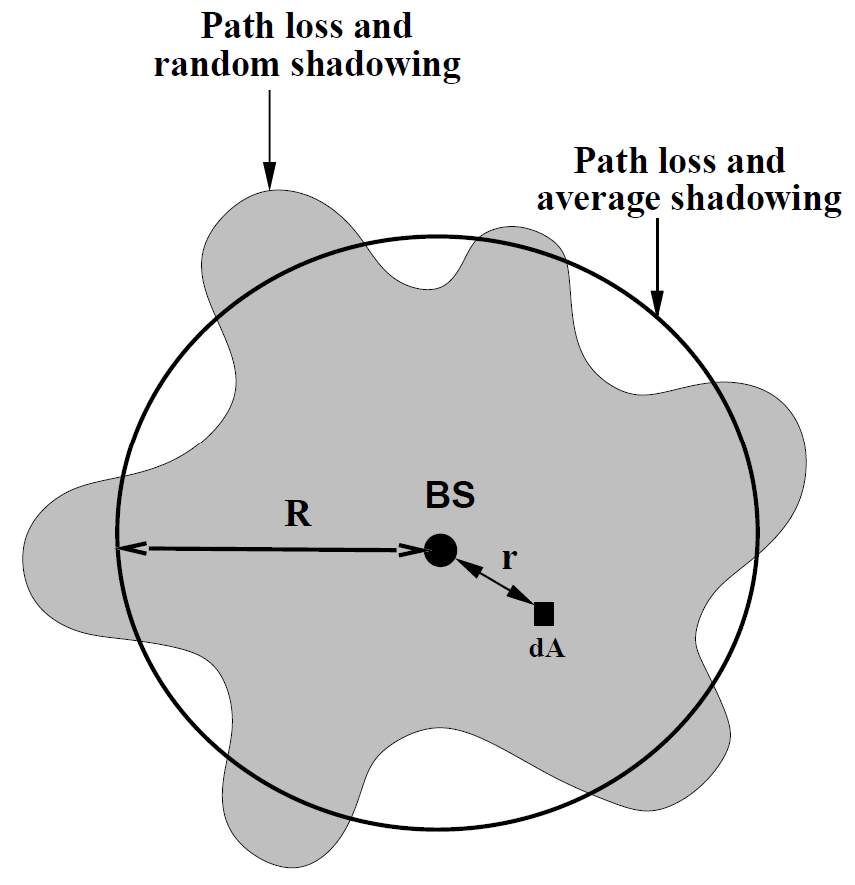
\includegraphics[width=0.4\textwidth]{fig/fig10.png}
		\caption{Illustration af cellulær dækning påvirket af path loss og shadowing. Figuren viser, hvordan shadowing resulterer i uregelmæssige konturer for modtaget signalstyrke i en cirkulær celle med radius \(R\).}
	\end{figure}
	\clearpage
	\subsection{Matematisk Modellering af Dækningen}
	Dækningen \( C \) i cellen defineres som det forventede areal, hvor den modtagne effekt \( P_r \) overstiger \( P_{\text{min}} \). Dette kan formelt beregnes ved at integrere over alle de områder \( dA \) i cellen, hvor dette krav er opfyldt:
	
	\[
	C = E\left[\frac{1}{\pi R^2} \int_{\text{cell area}} 1[P_r(r) > P_{\text{min}} \text{ in dA}] dA\right]
	\]
	
	I dette udtryk repræsenterer \( 1[\cdot] \) en indikatorfunktion, som er 1, når betingelsen indenfor klammen er sand, og ellers 0. Dette betyder, at vi kun tæller de områder med, hvor \( P_r(r) > P_{\text{min}} \). Da dækningen kan variere inden for cellen, er det nødvendigt at tage et gennemsnit (forventningsværdi) over hele cellens areal.
	
	\subsection{Outage Probability}
	Et beslægtet begreb er outage probability, som er den sandsynlighed, at den modtagne effekt \( P_r \) falder under \( P_{\text{min}} \) i et givet område af cellen. Dette kan udtrykkes som:
	
	\[
	p_{\text{out}}(P_{\text{min}}, r) = 1 - Q\left(\frac{P_{\text{min}} - \left(P_t + 10 \log_{10} K - 10 \gamma \log_{10}(r/d_0)\right)}{\sigma_{\psi_{\text{dB}}}}\right)
	\]
	
	Her er \( Q(\cdot) \) den komplementære fejlfunktion, som beregner sandsynligheden for, at en normalfordelt variabel overskrider en given værdi. Outage probability beskriver altså den del af celleområdet, hvor signalet ikke er stærkt nok til at sikre en pålidelig forbindelse.
	
	\subsection{Eksempler}
	
	\subsubsection{Eksempel 1: Beregning af Cell Coverage Area}
	
	Lad os antage, at vi har følgende parametre:
	\begin{itemize}
		\item Basestationens sendestyrke \( P_t = 100 \) mW (20 dBm)
		\item Modtagerens minimumskrav til signalstyrke \( P_{\text{min}} = -110 \) dBm
		\item Cellens radius \( R = 600 \) meter
		\item Path loss exponent \( \gamma = 3.71 \)
		\item Shadowing standard deviation \( \sigma_{\psi_{\text{dB}}} = 3.65 \) dB
	\end{itemize}
	
	Vi vil beregne dækningsområdet \( C \) ved brug af ligning (2.61):
	
	\[
	C = \frac{1}{2} + \frac{1}{2} \exp \left( \frac{2}{b^2} \right) Q \left( \frac{2}{b} \right),
	\]
	
	hvor \( a = \frac{P_{\text{min}} - P_R(R)}{\sigma_{\psi_{\text{dB}}}} \) og \( b = \frac{10 \gamma \log_{10}(e)}{\sigma_{\psi_{\text{dB}}}} \).
	
	\subsubsection{Eksempel 2: Beregning af Outage Probability}
	
	Antag, at vi ønsker at beregne outage probability for en bruger placeret 150 meter fra basestationen. Vi bruger følgende parametre:
	\begin{itemize}
		\item Basestationens sendestyrke \( P_t = 10 \) mW (10 dBm)
		\item Modtagerens minimumskrav til signalstyrke \( P_{\text{min}} = -110.5 \) dBm
		\item Afstand til basestationen \( d = 150 \) meter
		\item Path loss exponent \( \gamma = 3.71 \)
		\item Shadowing standard deviation \( \sigma_{\psi_{\text{dB}}} = 3.65 \) dB
	\end{itemize}
	
	Outage probability beregnes som:
	
	\[
	p_{\text{out}} = 1 - Q\left(\frac{-110.5 - \left(10 - 31.54 - 37.1 \log_{10}(150)\right)}{3.65}\right)
	\]
	
	\subsubsection{Eksempel 3: Beregning af Total Coverage Area}
	
	Hvis vi skal finde den totale dækningsgrad for cellen, hvor både path loss og shadowing er inkluderet, og vi har flere brugere jævnt fordelt i cellen, kan vi gentage beregningerne fra de tidligere eksempler for flere afstande og beregne gennemsnittet af disse resultater.
	
	\chapter{Appendix A - Båndpas Signaler og Kanaler}
	\section{Båndpas Signaler}
	I mange kommunikationssystemer bruges båndpas-signaler. Disse signaler har et frekvenssvar, der er koncentreret omkring en bærefrekvens \( f_c \) og en båndbredde \( 2B \), hvor \( B \) er meget mindre end \( f_c \). Figuren \ref{fig:BandpassSignal} viser, hvordan frekvensspektret af et båndpas-signal ser ud.
	
	\begin{figure}[h!]
		\centering
		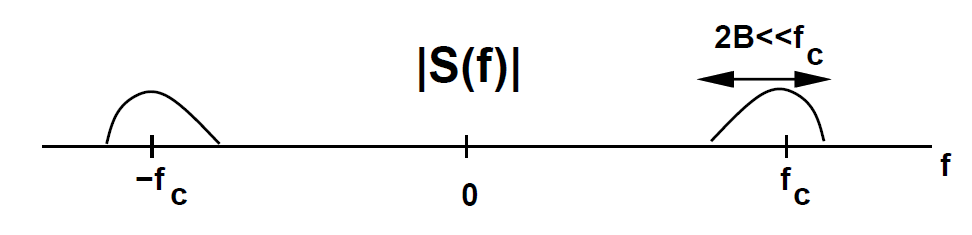
\includegraphics[width=0.6\textwidth]{fig/fig11.png}
		\caption{Båndpas signal \( S(f) \) med båndbredde \( 2B \) omkring bærefrekvensen \( f_c \).}
		\label{fig:BandpassSignal}
	\end{figure}
	
	\subsubsection{Repræsentation af Båndpas-Signaler}
	Et båndpas-signal er en kombination af to lavpas-signaler: en in-phase komponent \( s_I(t) \) og en kvadraturkomponent \( s_Q(t) \). Vi kan beskrive signalet ved hjælp af cosinus og sinus som:
	\[
	s(t) = s_I(t) \cos(2\pi f_c t) - s_Q(t) \sin(2\pi f_c t)
	\]
	Her er \( s_I(t) \) og \( s_Q(t) \) de lavpas-signaler, der indeholder informationen, mens \( \cos(2\pi f_c t) \) og \( \sin(2\pi f_c t) \) modulerer dem omkring bærefrekvensen \( f_c \).
	\newline\newline\noindent
	For at gøre det enklere at analysere, repræsenterer vi ofte et båndpas-signal med et \textbf{kompleks lavpas-signal}. Dette kompleks signal kaldes \( u(t) \) og beskriver signalets amplitude og fase:
	\[
	u(t) = s_I(t) + j s_Q(t)
	\]
	Den in-phase del \( s_I(t) \) er den reelle del, og kvadraturkomponenten \( s_Q(t) \) er den imaginære del. Sammen udgør de det komplette signal. Med dette kan vi omskrive båndpas-signalet som:
	\[
	s(t) = \Re \left\{ u(t) e^{j 2 \pi f_c t} \right\}
	\]
	hvor \( \Re \left\{ \cdot \right\} \) betyder, at vi tager den reelle del af det komplekse udtryk.
	
	\subsection{Amplitude og Fase af Signal}
	For at forstå, hvordan signalet varierer over tid, kan vi udtrykke dets amplitude \( a(t) \) og fase \( \phi(t) \). Amplituden er længden af signalvektoren, og den kan findes ved:
	\[
	a(t) = \sqrt{s_I^2(t) + s_Q^2(t)}
	\]
	Fasen \( \phi(t) \), som viser signalets vinkel, kan findes ved:
	\[
	\phi(t) = \tan^{-1} \left( \frac{s_Q(t)}{s_I(t)} \right)
	\]
	Således kan båndpas-signalet også skrives som:
	\[
	s(t) = a(t) \cos(2 \pi f_c t + \phi(t))
	\]
	Her er \( a(t) \) signalets amplitude, og \( \phi(t) \) er faseindhyllingen.
	
	\subsection{Frekvenssvar og Kanaler}
	I mange kommunikationssystemer er det vigtigt at forstå, hvordan signalet opfører sig, når det går gennem en kanal. En kanal kan ændre både amplituden og fasen af signalet. Kanalens frekvensrespons, \( H(f) \), beskriver, hvordan forskellige frekvenser påvirkes, og for båndpas-signaler kan dette repræsenteres som:
	\[
	H(f) = H_I(f - f_c) + j H_Q(f - f_c)
	\]
	hvor \( H_I(f) \) er den in-phase del af kanalens respons, og \( H_Q(f) \) er kvadraturdelen. Dette betyder, at både amplitude og fase af signalet kan ændres afhængigt af frekvensen.
	
	\subsubsection{Opsummering}
	Ved at repræsentere båndpas-signaler med deres komplekse lavpasækvivalenter kan vi forenkle analysen af både signaler og kanaler. Ved at forstå amplitudeindhyllingen \( a(t) \) og faseindhyllingen \( \phi(t) \) kan vi beskrive, hvordan signalet varierer over tid og gennem forskellige kanaler.
	\newline\newline\noindent
	Denne tilgang gør det lettere at analysere komplekse systemer, hvor signalet påvirkes af både amplitude- og faseændringer, såsom i trådløse kommunikationssystemer.
	
	
	\chapter{Appendix B - Probability Theory, Random Variables, and Random Processes}
	\section{Probability Theory}
	Sandsynlighedsteori giver en matematisk beskrivelse af tilfældige hændelser. Sådanne hændelser defineres i et underliggende sandsynlighedsområde \( (\Omega, \mathcal{E}, p(\cdot)) \), hvor \( \Omega \) er mængden af mulige udfald for tilfældige hændelser, og \( \mathcal{E} \) er en samling af delmængder af \( \Omega \), kaldet de tilfældige hændelser. Sandsynlighedsfordelingen \( p(A) \) er defineret for hver hændelse \( A \in \mathcal{E} \), hvor \( p(A) \) er sandsynligheden for hændelsen \( A \). For at definere et korrekt sandsynlighedsområde skal mængden \( \mathcal{E} \) være en \(\sigma\)-algebra, hvilket betyder, at den indeholder alle nødvendige operationer som foreninger, skæringer og komplementer.
	
	Sandsynlighedsfordelingen opfylder følgende grundlæggende egenskaber:
	\begin{enumerate}
		\item \( p(\Omega) = 1 \)
		\item \( 0 \leq p(A) \leq 1 \) for enhver hændelse \( A \in \mathcal{E} \)
		\item Hvis \( A \) og \( B \) er disjunkte hændelser, så gælder \( p(A \cup B) = p(A) + p(B) \)
	\end{enumerate}
	
	Unionen af flere hændelser kan beskrives ved følgende formel, også kaldet unionens lov:
	\[
	p(A_1 \cup A_2 \cup \ldots \cup A_n) = \sum_{i=1}^{n} p(A_i)
	\]
	Hvis to hændelser ikke overlapper, kan deres sandsynligheder blot lægges sammen.
	
	\section{Conditional Probability and Bayes' Rule}
	
	Når en hændelse \( A \) har fundet sted, kan vi betragte sandsynligheden for en anden hændelse \( B \), givet \( A \). Denne betingede sandsynlighed defineres som:
	\[
	p(B|A) = \frac{p(A \cap B)}{p(A)}
	\]
	Dette betyder, at sandsynligheden for \( B \), givet \( A \), normaliserer sandsynligheden for \( B \) i forhold til hændelsen \( A \). Bayes' sætning er en vigtig anvendelse af betinget sandsynlighed, som udtrykker sandsynligheden for \( A \), givet \( B \), som:
	\[
	p(A|B) = \frac{p(B|A)p(A)}{p(B)}
	\]
	
	\section{Independence of Events}
	
	To hændelser \( A \) og \( B \) siges at være uafhængige, hvis deres samtidige forekomst opfylder betingelsen:
	\[
	p(A \cap B) = p(A)p(B)
	\]
	Dette betyder, at forekomsten af den ene hændelse ikke påvirker sandsynligheden for den anden hændelse.
	
	\section{Sammenfatning af vigtig notation}
	
	\begin{itemize}
		\item \( p(A) \): Sandsynligheden for hændelse \( A \).
		\item \( p(A|B) \): Betinget sandsynlighed for \( A \) givet \( B \).
		\item \( \cap \): Skæringsmængden, dvs. de hændelser, som forekommer samtidigt.
		\item \( \cup \): Unionen, dvs. de hændelser, hvor enten den ene, den anden, eller begge forekommer.
	\end{itemize}
	
	Denne sandsynlighedsteori danner grundlaget for at analysere tilfældige variable og processer, som er vigtige i både kommunikationssystemer og statistiske modeller.
	
	\section{Probability Theory}
	Sandsynlighedsteori giver en matematisk ramme til at beskrive tilfældige hændelser. Et sandsynlighedsrum defineres som \((\Omega, \mathcal{E}, p)\), hvor:
	\begin{itemize}
		\item \( \Omega \) er \textbf{udfaldsrummet}, som indeholder alle mulige udfald af et eksperiment,
		\item \( \mathcal{E} \) er et \textbf{hændelsesrum}, som består af alle delmængder \( A \subseteq \Omega \), der beskriver mulige hændelser,
		\item \( p \) er en \textbf{sandsynlighedsfunktion}, der tilskriver en sandsynlighed til hver hændelse \( A \in \mathcal{E} \).
	\end{itemize}
	Sandsynlighedsfunktionen opfylder følgende grundlæggende egenskaber:
	\begin{enumerate}
		\item \( p(\Omega) = 1 \) (sandsynligheden for hele udfaldsrummet er 1),
		\item \( 0 \leq p(A) \leq 1 \) for enhver hændelse \( A \in \mathcal{E} \) (sandsynligheden for en hændelse ligger mellem 0 og 1),
		\item Hvis \( A \) og \( B \) er disjunkte hændelser (der ikke overlapper), gælder \( p(A \cup B) = p(A) + p(B) \).
	\end{enumerate}
	
	\subsection{Betinget Sandsynlighed og Uafhængighed}
	Betinget sandsynlighed definerer sandsynligheden for hændelse \( B \), givet at hændelse \( A \) er sket, og udtrykkes som:
	\[
	p(B | A) = \frac{p(A \cap B)}{p(A)} \quad \text{for} \quad p(A) \neq 0.
	\]
	Bayes' sætning er en vigtig anvendelse af betinget sandsynlighed:
	\[
	p(A | B) = \frac{p(B | A)p(A)}{p(B)}.
	\]
	To hændelser \( A \) og \( B \) er uafhængige, hvis \( p(A \cap B) = p(A)p(B) \), hvilket betyder, at den ene hændelses opståen ikke påvirker den andens.
	
	\section{Random Variables}
	En \textbf{tilfældig variabel} \( X \) er en funktion, der kortlægger udfald fra et eksperiment til reelle tal. En tilfældig variabel kan være enten:
	\begin{itemize}
		\item \textbf{Diskret}, hvis den kun kan antage bestemte værdier, f.eks. resultatet af et terningekast,
		\item \textbf{Kontinuerlig}, hvis den kan antage enhver værdi inden for et interval, f.eks. temperatur.
	\end{itemize}
	
	\subsection{Sandsynlighedstæthedsfunktion (PDF) og Kumulativ Fordelingsfunktion (CDF)}
	For en kontinuerlig tilfældig variabel \( X \) beskriver sandsynlighedstæthedsfunktionen (PDF) \( p_X(x) \) sandsynligheden for, at \( X \) falder i et givet interval, mens den kumulative fordelingsfunktion (CDF) \( P_X(x) \) beskriver sandsynligheden for, at \( X \) er mindre end eller lig med \( x \). De to funktioner er relateret som følger:
	\[
	P_X(x) = \mathbb{P}(X \leq x) = \int_{-\infty}^{x} p_X(t) dt,
	\]
	hvor \( P_X(x) \) er CDF'en og \( p_X(x) \) er PDF'en. Sandsynlighedstæthedsfunktionen opfylder:
	\[
	\int_{-\infty}^{\infty} p_X(x) dx = 1.
	\]
	
	\subsection{Forventningsværdi og Varians}
	Den \textbf{forventede værdi} (eller middelværdi) af en tilfældig variabel \( X \), betegnet \( \mathbb{E}[X] \), er den gennemsnitlige værdi af \( X \) og er givet ved:
	\[
	\mu_X = \mathbb{E}[X] = \int_{-\infty}^{\infty} x \, p_X(x) \, dx.
	\]
	\textbf{Variansen} af \( X \), der måler spredningen af værdierne omkring middelværdien, defineres som:
	\[
	\text{Var}(X) = \mathbb{E}[(X - \mu_X)^2] = \mathbb{E}[X^2] - \mu_X^2.
	\]
	Standardafvigelsen \( \sigma_X \) er kvadratroden af variansen.
	
	\subsection{Karakteristisk Funktion}
	Den karakteristiske funktion for \( X \), betegnet \( \phi_X(v) \), bruges til at studere summen af tilfældige variable og er defineret som Fourier-transformationen af PDF'en:
	\[
	\phi_X(v) = \mathbb{E}[e^{jvX}] = \int_{-\infty}^{\infty} p_X(x) e^{jvx} dx.
	\]
	Man kan genfinde PDF'en fra den karakteristiske funktion ved hjælp af invers Fourier-transformation:
	\[
	p_X(x) = \frac{1}{2\pi} \int_{-\infty}^{\infty} \phi_X(v) e^{-jvx} dv.
	\]
	
	\subsection{Korrelation og Kovarians}
	\textbf{Korrelationen} mellem to tilfældige variable \( X \) og \( Y \) er forventningen af deres produkt:
	\[
	\text{Corr}(X, Y) = \mathbb{E}[XY].
	\]
	\textbf{Kovariansen} måler, hvor meget \( X \) og \( Y \) varierer sammen, og er defineret som:
	\[
	\text{Cov}(X, Y) = \mathbb{E}[(X - \mu_X)(Y - \mu_Y)].
	\]
	Hvis \( \text{Cov}(X, Y) = 0 \), siges \( X \) og \( Y \) at være ukorrelerede.
	
	\section{Gaussisk Fordeling}
	Den \textbf{Gaussiske fordeling} (eller normalfordeling) er en vigtig fordeling, som ofte anvendes i praksis. PDF'en for en Gaussisk fordeling er givet ved:
	\[
	p_X(x) = \frac{1}{\sqrt{2\pi \sigma_X^2}} \exp\left( - \frac{(x - \mu_X)^2}{2 \sigma_X^2} \right),
	\]
	hvor:
	\begin{itemize}
		\item \( \mu_X \) er middelværdien af fordelingen,
		\item \( \sigma_X^2 \) er variansen,
		\item \( \exp(\cdot) \) er eksponentialfunktionen.
	\end{itemize}
	
	\subsection{Kumulativ Fordelingsfunktion (CDF)}
	Den kumulative fordelingsfunktion for en Gaussisk fordeling kan ikke udtrykkes i lukket form, men kan beregnes ved hjælp af Gauss' Q-funktion:
	\[
	P_X(x) = 1 - Q\left( \frac{x - \mu_X}{\sigma_X} \right),
	\]
	hvor Q-funktionen er defineret som:
	\[
	Q(x) = \frac{1}{\sqrt{2\pi}} \int_x^{\infty} \exp\left( -\frac{y^2}{2} \right) dy.
	\]
	
	\subsection{Q-funktion}
	Den Gaussiske Q-funktion beskriver sandsynligheden for, at en normalfordelt variabel overskrider en given værdi \( x \). Funktionen er relateret til den komplementære fejlfunktion og anvendes ofte i kommunikationsteori til at modellere fejl:
	\[
	Q(x) \triangleq \frac{1}{\sqrt{2\pi}} \int_x^{\infty} e^{-y^2/2} \, dy.
	\]
	
	\section{Tilfældige Variable og Prøverum}
	En tilfældig variabel \( X \) beskriver udfald af et eksperiment og kan antage forskellige værdier afhængig af udfaldet. Prøverummet \( \Omega \) er mængden af alle mulige udfald, og en tilfældig variabel kan kortlægge udfald fra prøverummet til den reelle linje \( \mathbb{R} \). For eksempel, hvis vi kaster en terning, er prøverummet \( \Omega = \{1, 2, 3, 4, 5, 6\} \), og en tilfældig variabel kunne kortlægge disse udfald til nogle talværdiers forventede gennemsnit.
	
	\chapter{Appendix C - Matrix Definitions and Operations}
	
	\section{Matrices and Vectors}
	En \(N \times M\) matrix \(A\) er en rektangulær samling af værdier med \(N\) rækker og \(M\) kolonner, skrevet som:
	
	\[
	A = \begin{bmatrix} 
		a_{11} & \dots & a_{1M} \\
		\vdots & \ddots & \vdots \\
		a_{N1} & \dots & a_{NM} 
	\end{bmatrix}.
	\]
	Den \(ij\)-te element (eller indgang) i \(A\), dvs. elementet i den \(i\)-te række og \(j\)-te kolonne, betegnes \(A_{ij}\). En \(N \times M\) matrix med \(N = M\) kaldes en \textbf{kvadratisk matrix}, mens en matrix med \(N > M\) kaldes en \textbf{smal matrix}, og en matrix med \(N < M\) kaldes en \textbf{bred matrix}.
	\newline\newline
	De \textbf{diagonale elementer} i en kvadratisk matrix er de elementer, der ligger langs diagonal-linjen fra øverste venstre til nederste højre, dvs. elementerne \(A_{ii}\) for \(i = j\). \textbf{Spor} af en kvadratisk matrix \(A\) defineres som summen af dens diagonale elementer: 
	\[
	\text{Tr}[A] = \sum_{i=1}^{N} A_{ii}.
	\]
	
	En kvadratisk matrix kaldes en \textbf{diagonal matrix}, hvis alle elementer, der ikke er på diagonalen, er nul: \(A_{ij} = 0, i \neq j\).
	\newline\newline
	En \textbf{identitetsmatrix} \(I_N\) er en diagonal matrix, hvor alle diagonale elementer er lig med 1: \(I_{ii} = 1\) for \(i = 1, \dots, N\). 
	\newline\newline
	En matrix med kun én kolonne (\(M = 1\)) kaldes en \textbf{kolonnevektor}, eller blot en \textbf{vektor}. Antallet af rækker i en vektor er dens dimension. For eksempel er en \(N\)-dimensionel vektor \(x\) givet ved:
	
	\[
	x = \begin{bmatrix} 
		x_1 \\
		\vdots \\
		x_N 
	\end{bmatrix}.
	\]
	
	Vektorens \(i\)-te element betegnes som \(x_i\). En vektor, hvor alle elementer er lig med 1, kaldes en \textbf{enhedsvektor} \(1_N\). 
	
	\subsection{Matrix og Vektor Operationer}
	Transponeringen af en matrix \(A\), betegnet \(A^T\), opnås ved at bytte rækker og kolonner:
	\[
	A^T = \begin{bmatrix} 
		a_{11} & \dots & a_{N1} \\
		\vdots & \ddots & \vdots \\
		a_{1M} & \dots & a_{NM} 
	\end{bmatrix}.
	\]
	Transponeringen af en vektor \(x\) er skrevet som \(x^T = [x_1 \dots x_N]\).
	
	Den \textbf{komplekse konjugerede} af en matrix \(A\), betegnet \(A^*\), opnås ved at tage den komplekse konjugerede af hvert element i \(A\):
	\[
	A^* = \begin{bmatrix} 
		a_{11}^* & \dots & a_{1M}^* \\
		\vdots & \ddots & \vdots \\
		a_{N1}^* & \dots & a_{NM}^* 
	\end{bmatrix}.
	\]
	
	En kvadratisk matrix \(A\) er \textbf{Hermitesk}, hvis \(A = A^H = (A^*)^T\). En Hermitesk matrix er symmetrisk med hensyn til transponering af komplekse konjugerede elementer.
	
	\subsection{Addition og Subtraktion af Matricer}
	To \(N \times M\) matricer kan adderes eller subtraheres, hvis deres dimensioner er ens. Addition og subtraktion foretages elementvis:
	\[
	C = A + B, \quad C_{ij} = A_{ij} + B_{ij}.
	\]
	
	\subsection{Multiplikation af Matricer}
	To matricer kan multipliceres, hvis antallet af kolonner i den første matrix er lig med antallet af rækker i den anden. Hvis \(A\) er en \(N \times K\) matrix, og \(B\) er en \(K \times M\) matrix, er produktet \(C = AB\) en \(N \times M\) matrix, hvor:
	\[
	C_{ij} = \sum_{k=1}^{K} A_{ik} B_{kj}.
	\]
	Matrixmultiplikation er ikke kommutativ, dvs. generelt gælder det, at \(AB \neq BA\).
	
	\subsection{Determinant og Invers Matrix}
	Determinanten af en \(2 \times 2\) matrix \(A\) defineres som:
	\[
	\text{det}(A) = a_{11} a_{22} - a_{12} a_{21}.
	\]
	En \(N \times N\) kvadratisk matrix er \textbf{inverterbar}, hvis dens determinant er forskellig fra nul. Inversen af \(A\), betegnet \(A^{-1}\), er defineret som den matrix, der opfylder:
	\[
	A A^{-1} = I_N.
	\]
	Inversen af en \(2 \times 2\) matrix \(A\) er givet ved:
	\[
	A^{-1} = \frac{1}{\text{det}(A)} \begin{bmatrix} 
		a_{22} & -a_{12} \\
		-a_{21} & a_{11} 
	\end{bmatrix}.
	\]
	
	\subsection{Løsning af Lineære Ligninger}
	Matrixinverser bruges ofte til at løse systemer af lineære ligninger. For et system af ligninger \(Ax = y\), hvor \(A\) er en inverterbar matrix, findes løsningen som:
	\[
	x = A^{-1}y.
	\]
	Hvis \(A\) ikke er inverterbar, findes der muligvis ingen unik løsning.
	
	\section{Matrices and Vectors}
	En \(N \times M\) matrix \(A\) er en rektangulær tabel af værdier med \(N\) rækker og \(M\) kolonner, skrevet som:
	\[
	A = \begin{bmatrix}
		a_{11} & \cdots & a_{1M} \\
		\vdots & \ddots & \vdots \\
		a_{N1} & \cdots & a_{NM}
	\end{bmatrix}.
	\]
	Elementet i \(i\)-te række og \(j\)-te kolonne af \(A\) skrives som \(A_{ij}\), hvor \(A_{ij} = a_{ij}\). En \(N \times M\) matrix kaldes en firkantet matrix, hvis \(N = M\). Hvis \(N > M\) kaldes den en tynd matrix, og hvis \(N < M\), en bred matrix.
	
	De diagonale elementer i en firkantet matrix er elementerne langs diagonalen fra øverste venstre til nederste højre. Diagonalelementerne \(A_{ii}\) med \(i = j\) spiller en vigtig rolle. Sporet af en firkantet matrix, kaldet \(\text{Tr}[A]\), er summen af alle diagonale elementer: \(\text{Tr}[A] = \sum_{i=1}^{N} A_{ii}\).
	
	\textbf{Specielle matricer:}
	- En diagonal matrix har kun ikke-nul elementer på diagonalen.
	- En øvre trekantet matrix har alle nul elementer under diagonalen, mens en nedre trekantet matrix har alle nul elementer over diagonalen.
	- En identitetsmatrix \(I_N\) er en diagonal matrix med alle diagonale elementer lig med 1.
	
	En matrix med én kolonne, dvs. \(M = 1\), kaldes en kolonnevektor. En matrix med én række kaldes en rækkevektor.
	
	Vektorer med dimension \(N\) skrives ofte som:
	\[
	\mathbf{x} = \begin{bmatrix}
		x_1 \\
		\vdots \\
		x_N
	\end{bmatrix}.
	\]
	Normen af en vektor \(\mathbf{x}\) defineres som:
	\[
	||\mathbf{x}|| = \sqrt{\sum_{i=1}^{N} x_i^2}.
	\]
	
	\section{Matrix and Vector Operations}
	Transponeringen af en matrix \(A\), skrevet som \(A^T\), opnås ved at bytte rækkerne og kolonnerne. Transponeringen af en vektor \(\mathbf{x}\) bliver en rækkevektor:
	\[
	A^T = \begin{bmatrix}
		a_{11} & a_{N1} \\
		\vdots & \ddots \\
		a_{1M} & a_{NM}
	\end{bmatrix}.
	\]
	Kompleks konjugation af en matrix \(A\) betegnes \(A^*\) og fås ved at tage kompleks konjugat af hvert element. Hermitisk transponering af en matrix \(A\) skrives som \(A^H = (A^*)^T\), og en hermitisk matrix opfylder \(A = A^H\).
	
	To matricer \(A\) og \(B\) kan lægges sammen element for element:
	\[
	C = A + B,\quad C_{ij} = A_{ij} + B_{ij}.
	\]
	Multiplikation af en matrix med en skalar \(k\) skrives som \(kA\), og hvert element i matrixen ganges med \(k\).
	
	\textbf{Matrixmultiplikation:} To matricer \(A\) og \(B\) kan multipliceres, hvis antallet af kolonner i \(A\) er lig med antallet af rækker i \(B\). Produktet \(AB\) er en matrix, hvor elementet \(C_{ij}\) er givet ved:
	\[
	C_{ij} = \sum_{k=1}^{M} A_{ik} B_{kj}.
	\]
	
	\textbf{Matrix inversion:} Inversen af en \(N \times N\) matrix \(A\), hvis den eksisterer, betegnes som \(A^{-1}\), og opfylder \(AA^{-1} = I_N\). Hvis en matrix ikke er invertibel, kaldes den singulær.
	
	\section{Matrix Decompositions}
	En vigtig egenskab ved firkantede matricer er deres egenværdier og egenvektorer. En egenværdi \(\lambda\) er en skalar, for hvilken der eksisterer en ikke-nul vektor \(\mathbf{x}\), så \(A\mathbf{x} = \lambda\mathbf{x}\). Vektoren \(\mathbf{x}\) kaldes egenvektoren tilhørende egenværdien \(\lambda\).
	
	\textbf{Singular værdi dekomposition (SVD):} Enhver matrix \(A\) kan nedbrydes som:
	\[
	A = U\Sigma V^H,
	\]
	hvor \(U\) og \(V\) er unitære matricer, og \(\Sigma\) er en diagonal matrix med singularværdier.
	
	\textbf{Determinanten:} For en firkantet matrix \(A\) er determinanten givet ved:
	\[
	\det[A] = \sum_{i=1}^{N} a_{ij} (-1)^{i+j} \det[A_{ij}],
	\]
	hvor \(A_{ij}\) er underdeterminanten opnået ved at slette \(i\)-te række og \(j\)-te kolonne.
	
	\chapter{Appendix D}
	
	\chapter{Statistical Multipath Channel Models}
	\textbf{Multipath Fading og Channel models}
	\newline\noindent
	I dette kapitel undersøger vi fading-modeller, der beskriver, hvordan signaler kan blive forstærket eller svækket, når de bevæger sig gennem forskellige \textit{multipath} komponenter i en kanal. Mens vi i kapitel \ref{cha:Free-Space Path Loss og Doppler-effekt} talte om \textit{ray-tracing} modeller for deterministiske kanaler, kræver virkelige omgivelser ofte en statistisk tilgang. Deterministiske modeller er sjældent anvendelige, så vi bliver nødt til at karakterisere kanalen statistisk. I dette kapitel vil vi modellere \textit{multipath}-kanalen ved hjælp af en tilfældig, tidsvarierende \textit{impulse response}, og vi vil beskrive dens vigtige egenskaber.
	\newline\newline
	Når et signal transmitteres gennem en \textit{multipath} kanal, vil modtageren opfatte det som en række af pulser. Hver puls svarer enten til det direkte \textit{line-of-sight (LOS)} signal eller et reflekteret \textit{multipath} signal fra forskellige \textit{scatterers} eller grupper af \textit{scatterers}. En vigtig egenskab ved en \textit{multipath} kanal er \textit{delay spread}, som måler tidsforskellen mellem det første ankomne signal (enten \textit{LOS} eller \textit{multipath}) og det sidste ankomne signal fra den samme transmitterede puls. Hvis \textit{delay spread} er lille sammenlignet med den inverse af signalets båndbredde, vil der være minimal tidsudbredning i det modtagne signal. Men hvis \textit{delay spread} er stor, vil der være betydelig tidsudbredning, hvilket kan føre til væsentlig forvrængning af signalet.
	\newline\newline
	En anden vigtig egenskab ved \textit{multipath} kanalen er dens tidsvarierende natur. Denne variation opstår, når enten senderen eller modtageren bevæger sig, hvilket betyder, at reflektorer i signalvejen ændrer deres placering over tid. Dette medfører ændringer i amplitude, forsinkelse og antallet af \textit{multipath} komponenter, som modtageren opfatter. Hvis vi f.eks. transmitterer pulser gentagne gange fra en bevægende sender, vil vi observere ændringer i signalets styrke og forsinkelser over tid. Dog sker disse ændringer over en længere tidsskala end fading forårsaget af den konstruktive og destruktive tilføjelse af faste \textit{multipath} komponenter fra faste \textit{scatterers}.
	\newline\newline
	Vi vil starte med en generisk model for den tidsvarierende \textit{channel impulse response} for at fange både hurtige og langsomme variationer i kanalen. Derefter vil vi begrænse denne model til \textit{narrowband fading}, hvor kanalens båndbredde er lille i forhold til den inverse af \textit{delay spread}. For \textit{narrowband} modeller antager vi en kvasi-statisk situation, hvor vi har et fast antal \textit{multipath} komponenter, hver med fast \textit{path loss} og \textit{shadowing}. 
	
		
	\section{Tidsvarierende Kanalimpulsrespons}
	I trådløse kommunikationssystemer ændrer kanalen sig ofte over tid på grund af bevægelse fra enten senderen, modtageren eller objekter i miljøet. Disse ændringer kan have en væsentlig indvirkning på signalets kvalitet, og derfor er det vigtigt at kunne modellere, hvordan signalet ændrer sig, når det bevæger sig gennem en kanal, der varierer over tid.
	\newline\newline
	Kanalimpulsresponsen beskriver, hvordan signalet påvirkes af kanalen over tid. En kanal kan introducere forsinkelser, reflektere signalet fra forskellige objekter og påvirke signalets forstærkning (eller dæmpning). For at beskrive disse ændringer anvender vi ofte en flervejskanalmodel, hvor signalet modtages som summen af flere signaler, der hver har taget forskellige veje (flerveje) gennem miljøet.
	
	\subsection{Matematisk Modellering af Tidsvarierende Kanalimpulsrespons}
	Den matematiske model for en tidsvarierende kanalimpulsrespons er givet ved funktionen \(c(\tau, t)\), hvor:
	\begin{itemize}
		\item \( \tau \) repræsenterer forsinkelsen (delay) for en flervejskomponent.
		\item \( t \) er tiden, som viser ændringer i kanalen over tid.
	\end{itemize}
	
	Denne funktion beskriver kanalens respons på et signal, som udsendes ved tid \( t = 0 \). Den kan udtrykkes som en sum af forsinkede versioner af signalet, hvor hver version er vægtet med en faktor, der beskriver signalets dæmpning eller forstærkning langs den pågældende vej:
	
	\[
	c(\tau, t) = \sum_{n=0}^{N(t)-1} \alpha_n(t) \delta(\tau - \tau_n(t))
	\]
	hvor:
	\begin{itemize}
		\item \( N(t) \) er antallet af flervejskomponenter, der ændrer sig over tid,
		\item \( \alpha_n(t) \) er den komplekse forstærkning af den \( n \)-te flervejskomponent,
		\item \( \tau_n(t) \) er forsinkelsen for den \( n \)-te flervejskomponent,
		\item \( \delta(\tau - \tau_n(t)) \) er Dirac delta-funktionen, som beskriver impulsresponsen langs den \( n \)-te vej.
	\end{itemize}
	
	Dette betyder, at modtageren modtager flere forsinkede kopier af det samme signal, hvor hver kopi har forskellig forsinkelse og forstærkning.
	
	\begin{figure}[h!]
		\centering
		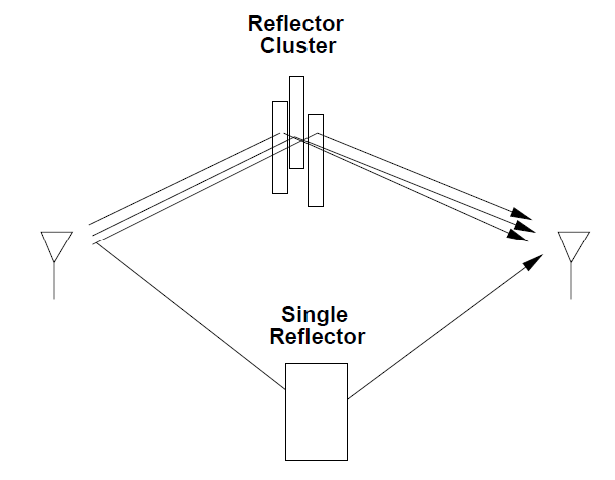
\includegraphics[width=0.7\textwidth]{fig/fig14.png}
		\caption{System med enkelt reflektor og reflektorklynge, som skaber flervejskomponenter.}
		\label{fig:reflector_cluster}
	\end{figure}
	
	\subsection{Kanalimpulsrespons ved Forskellige Tidspunkter}
	Lad os overveje systemet ved tidspunktet \( t_1 \), hvor vi kan repræsentere kanalimpulsresponsen som en sum af tre flervejskomponenter, hver med forsinkelse \( \tau_n \), amplitude \( \alpha_n \), og fase \( \phi_n \):
	\[
	c(\tau, t_1) = \sum_{n=0}^{2} \alpha_n(t_1) e^{-j \phi_n(t_1)} \delta(\tau - \tau_n(t_1))
	\]
	Her repræsenterer \( n=0 \) den direkte linje af synet (LOS), mens \( n=1 \) og \( n=2 \) repræsenterer reflekterede veje. Som vist i Figur \ref{fig:system_t1} modtages signalet ved tidspunktet \( t_1 \) som summen af disse tre signaler.
	
	\begin{figure}[h!]
		\centering
		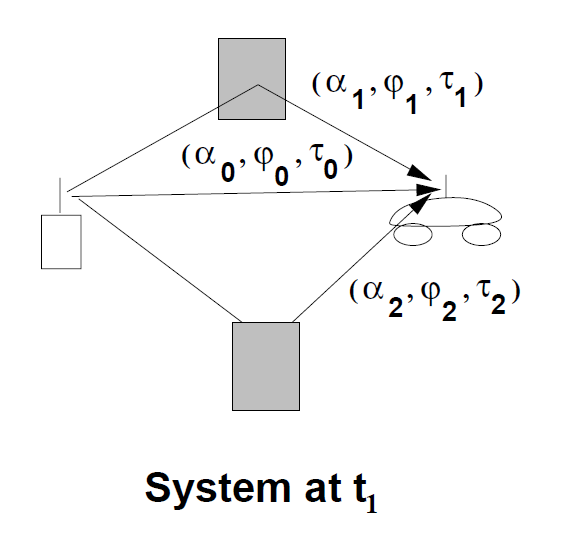
\includegraphics[width=0.7\textwidth]{fig/fig15.png}
		\caption{System ved tidspunktet \( t_1 \) med flervejskomponenterne defineret af \( (\alpha_i, \phi_i, \tau_i) \).}
		\label{fig:system_t1}
	\end{figure}
	
	Når systemet ændrer sig over tid, vil flervejskomponenternes parametre ændre sig. Ved tidspunktet \( t_2 \) modtages signalet som:
	\[
	c(\tau, t_2) = \sum_{n=0}^{2} \alpha_n'(t_2) e^{-j \phi_n'(t_2)} \delta(\tau - \tau_n'(t_2))
	\]
	som vist i Figur \ref{fig:system_t2}, der viser, hvordan flervejskomponenterne ændrer sig over tid.
	
	\begin{figure}[h!]
		\centering
		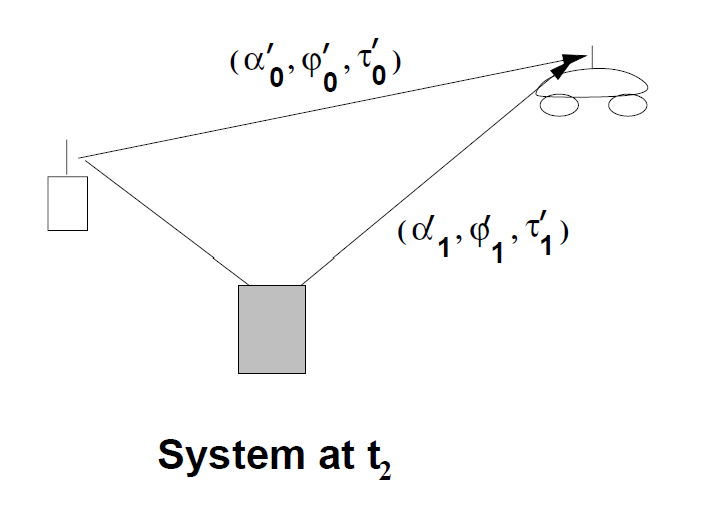
\includegraphics[width=0.7\textwidth]{fig/fig16.png}
		\caption{System ved tidspunktet \( t_2 \), hvor flervejskomponenterne har ændret sig til nye værdier \( (\alpha_i', \phi_i', \tau_i') \).}
		\label{fig:system_t2}
	\end{figure}
	
	\subsection{Tidsvarierende Kanalrespons i Frekvensdomænet}
	For at analysere kanalens opførsel i frekvensdomænet kan vi bruge Fourier-transformationen til at transformere kanalimpulsresponsen til frekvensdomænet. Det tidsvarierende frekvensrespons \( H(f, t) \) er givet ved:
	\[
	H(f, t) = \int_{-\infty}^{\infty} c(\tau, t) e^{-j 2 \pi f \tau} d\tau
	\]
	Denne ligning beskriver, hvordan kanalen opfører sig ved forskellige frekvenser \( f \) over tid \( t \).
	
	\subsection{Doppler-effekter}
	Når der er relativ bevægelse mellem sender og modtager, vil der være en Doppler-skift i frekvensen. Doppler-skiftet kan beregnes som:
	\[
	f_D = \frac{v}{\lambda} \cos(\theta)
	\]
	hvor:
	\begin{itemize}
		\item \( v \) er den relative hastighed mellem sender og modtager,
		\item \( \lambda \) er signalets bølgelængde,
		\item \( \theta \) er vinklen mellem bevægelsesretningen og signalets udbredelsesretning.
	\end{itemize}
	Denne effekt fører til frekvensskift i det modtagne signal, som skal tages i betragtning, når signalet modtages og behandles.
	\clearpage
	\subsection{Kanalens Ikke-Stationære Respons}
	Figur \ref{fig:nonstationary_channel} viser, hvordan kanalen ændrer sig over tid fra tidspunktet \( t_1 \) til \( t_2 \). Når kanalen ikke er stationær, ændrer forsinkelsen \( \tau \) sig løbende over tid, hvilket giver et tidsvarierende kanalrespons.
	\begin{figure}[h!]
		\centering
		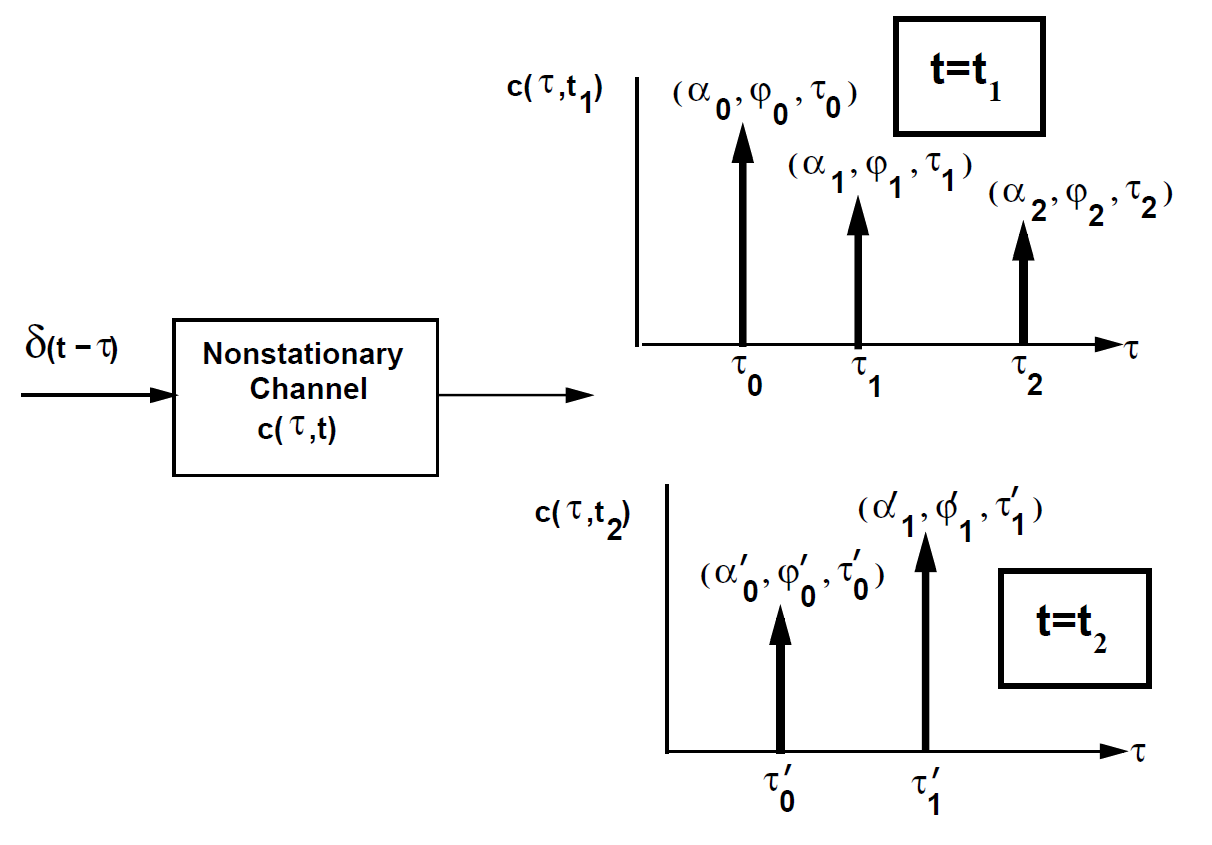
\includegraphics[width=0.7\textwidth]{fig/fig17.png}
		\caption{Tidsvarierende ikke-stationær kanalimpulsrespons ved tidspunkterne \( t_1 \) og \( t_2 \).}
		\label{fig:nonstationary_channel}
	\end{figure}
	
	\subsection*{Afslutning}
	Den tidsvarierende kanalimpulsrespons giver en omfattende model for, hvordan signalet ændrer sig, når det rejser gennem en trådløs kanal. Ved at tage højde for flervejseffekter, Doppler-skift og tidsvariationer kan vi bedre forstå og kompensere for de udfordringer, som trådløs kommunikation medfører.
	
	\subsubsection*{Eksempel 3.1: Trådløst LAN i fabriksmiljø}
	Overvej et trådløst LAN, der opererer i en fabrik i nærheden af et transportbånd. Senderen og modtageren har en \textit{line-of-sight} (LOS) sti imellem sig med en forstærkning \( \alpha_0 \), fase \( \phi_0 \) og forsinkelse \( \tau_0 \). Hvert \( T_0 \) sekund passerer et metalobjekt ned ad transportbåndet, hvilket skaber en ekstra reflekteret signalvej ud over LOS-stien, med en forstærkning \( \alpha_1 \), fase \( \phi_1 \) og forsinkelse \( \tau_1 \). Opgaven er at finde den tidsvarierende kanalimpulsrespons \( c(\tau, t) \) for denne kanal.
	
	\subsection*{Løsning:}
	For \( t \neq nT_0 \), hvor \( n = 1, 2, \dots \), svarer kanalens impulsrespons kun til LOS-stien. For \( t = nT_0 \) vil kanalens impulsrespons inkludere både LOS- og de reflekterede signalveje. Derfor er den tidsvarierende kanalimpulsrespons \( c(\tau, t) \) givet ved:
	
	\[
	c(\tau, t) =
	\begin{cases} 
		\alpha_0 e^{j \phi_0} \delta(\tau - \tau_0) & t \neq nT_0, \\
		\alpha_0 e^{j \phi_0} \delta(\tau - \tau_0) + \alpha_1 e^{j \phi_1} \delta(\tau - \tau_1) & t = nT_0.
	\end{cases}
	\]
	
	Dette betyder, at når \( t = nT_0 \), vil modtageren opfange både LOS-signalet og den reflekterede vej. Den reflekterede vej tilføjer en ekstra forsinkelse \( \tau_1 \) og forstærkning \( \alpha_1 \).
	
	\subsection*{Bemærkninger:}
	For typiske bærefrekvenser vil den \( n \)-te multipath-komponent have \( f_c \tau_n(t) \gg 1 \). For eksempel, med \( f_c = 1 \text{ GHz} \) og \( \tau_n = 50 \text{ ns} \) (en typisk værdi for et indendørs system), vil \( f_c \tau_n = 50 \gg 1 \). Dette betyder, at forsinkelsen \( 50 \text{ ns} \) er signifikant i forhold til bærefrekvensen, hvilket resulterer i en faseforskydning i det reflekterede signal. Denne faseforskydning skal tages i betragtning ved modellering af kanalen.
	
	\subsection*{Opsummering af løsningen:}
	\begin{itemize}
		\item Når \( t \neq nT_0 \), modtages kun LOS-signalet med impulsresponsen \( \alpha_0 e^{j \phi_0} \delta(\tau - \tau_0) \).
		\item Når \( t = nT_0 \), modtages både LOS- og den reflekterede signalvej, hvor den samlede impulsrespons indeholder både \( \alpha_0 e^{j \phi_0} \delta(\tau - \tau_0) \) og \( \alpha_1 e^{j \phi_1} \delta(\tau - \tau_1) \).
		\item Faseforskydningen mellem LOS og den reflekterede vej påvirker signalets kombination ved modtageren.
	\end{itemize}
	
	\clearpage
	
	
	\section{Narrow Fading Models}
	Når \textit{delay spread} \( T_m \) i en kanal er lille i forhold til den inverse signalbåndbredde \( B \) for det transmitterede signal, dvs. \( T_m \ll B^{-1} \), kan kanalen betragtes som en \textit{smalbånds fading} kanal. Som nævnt tidligere karakteriseres \textit{delay spread} typisk ved \textit{rms delay spread}, men kan også beskrives på andre måder. Under de fleste \textit{delay spread}-modeller gælder, at \( T_m \ll B^{-1} \), hvilket betyder, at forsinkelsen forbundet med den \( i \)-te multipath-komponent \( \tau_i \leq T_m \) for alle \( i \). Dette indebærer, at modtageren opfatter \( u(t) \) og \( u(t - \tau_i) \) som næsten identiske, dvs. \( u(t - \tau_i) \approx u(t) \) for små \( \tau_i \). Ligning (3.11) kan derfor omskrives som:
	
	\[
	r(t) = \Re \left\{ u(t) e^{j 2 \pi f_c t} \left( \sum_n \alpha_n(t) e^{-j \phi_n(t)} \right) \right\}.
	\]
	
	Her repræsenterer \( r(t) \) det modtagne signal, hvor \( u(t) \) er det komplekse basebandsignal og \( f_c \) er bærefrekvensen. Summationen inden for parenteserne repræsenterer alle de multipath-komponenter, som modtageren opfatter. Hver multipath-komponent \( \alpha_n(t) \) er vægtet med en kompleks forstærkning og faseforskydning \( \phi_n(t) \), som er relateret til forsinkelsen \( \tau_n(t) \) og Doppler-skiftet \( f_{D_n} \). 
	\newline\newline
	Ligningen for \(r(t)\) adskiller sig fra det oprindeligt transmitterede signal ved at inkludere en kompleks skalfaktor, som er uafhængig af det transmitterede signal \( s(t) \) eller basebandsignalet \( u(t) \), så længe smalbåndsantagelsen (narrow band) \( T_m \ll B^{-1} \) er opfyldt.
	
	\subsection{In-Phase og Quadrature Komponenter}
	For at karakterisere den tilfældige skalafaktor forårsaget af multipath vælger vi \( s(t) \) som en umoduleret bærebølge med en tilfældig faseoffset \( \phi_0 \):
	
	\[
	s(t) = \Re \left\{ e^{j \left( 2 \pi f_c t + \phi_0 \right)} \right\} = \cos \left( 2 \pi f_c t - \phi_0 \right),
	\]
	\noindent
	hvilket er et smalbåndssignal for ethvert \( T_m \).
	\newline\newline\noindent
	Med denne antagelse bliver det modtagne signal:
	
	\[
	r(t) = \Re \left\{ \left( \sum_{n=0}^{N(t)} \alpha_n(t) e^{-j \phi_n(t)} \right) e^{j 2 \pi f_c t} \right\} = r_I(t) \cos \left( 2 \pi f_c t \right) + r_Q(t) \sin \left( 2 \pi f_c t \right),
	\]
	\noindent
	hvor de \textit{in-phase} og \textit{quadrature} komponenter er givet ved:
	
	\[
	r_I(t) = \sum_{n=1}^{N(t)} \alpha_n(t) \cos \phi_n(t),
	\]
	\noindent
	og
	
	\[
	r_Q(t) = \sum_{n=1}^{N(t)} \alpha_n(t) \sin \phi_n(t),
	\]
	\noindent
	hvor faseforskydningen \( \phi_n(t) = 2\pi f_c \tau_n(t) - \phi_{D_n}(t) - \phi_0 \) nu inkluderer faseoffset \( \phi_0 \) såvel som effekterne af forsinkelse og Doppler.
	
	\subsection{Fading og Statistik}
	Hvis \( N(t) \) er stort, kan vi benytte Central Limit Theoremet og antage, at \( \alpha_n(t) \) og \( \phi_n(t) \) er stationære og ergodiske, så \( r_I(t) \) og \( r_Q(t) \) kan beskrives som fælles Gaussiske tilfældige processer. Den Gaussiske egenskab er også gældende for små \( N \), hvis \( \alpha_n(t) \) er Rayleigh-fordelte, og \( \phi_n(t) \) er jævnt fordelt mellem \( [-\pi, \pi] \). Dette sker, når den \( n \)-te multipath-komponent stammer fra et reflektionskluster med mange ikke-resolvable multipath-komponenter.
	\clearpage

	\subsection{Autokorrelation, krydskorrelation og spektraltæthed}
	
	Autokorrelation beskriver, hvordan værdierne af et signal på forskellige tidspunkter hænger sammen. I et \textit{multipath} miljø kan vi udlede autokorrelationen for in-phase $r_I(t)$ og kvadratur $r_Q(t)$ komponenterne ved at bruge deres statistiske uafhængighed og Doppler-skiftet.
	
	For at beregne autokorrelationen af $r_I(t)$ antager vi, at Doppler-forskydningen $f_D$ er jævnt fordelt over $[-\pi, \pi]$, og at hver multipath-komponent er uafhængig. Autokorrelationen af $r_I(t)$ er givet ved:
	
	\[
	A_{r_I}(\tau) = E[r_I(t)r_I(t + \tau)] = \sum_n E[\alpha_n^2] E[\cos(2\pi f_D \tau)],
	\]
	
	hvor $\alpha_n$ er amplituden af den $n$-te multipath komponent, og $\tau$ er tidsforskellen mellem de to signaler. 
	\newline\newline
	I et uniformt \textit{scattering environment}, som vist i Figur \ref{fig:uniform_scattering}, kan denne sum forenkles til:
	
	\begin{figure}[h!]
		\centering
		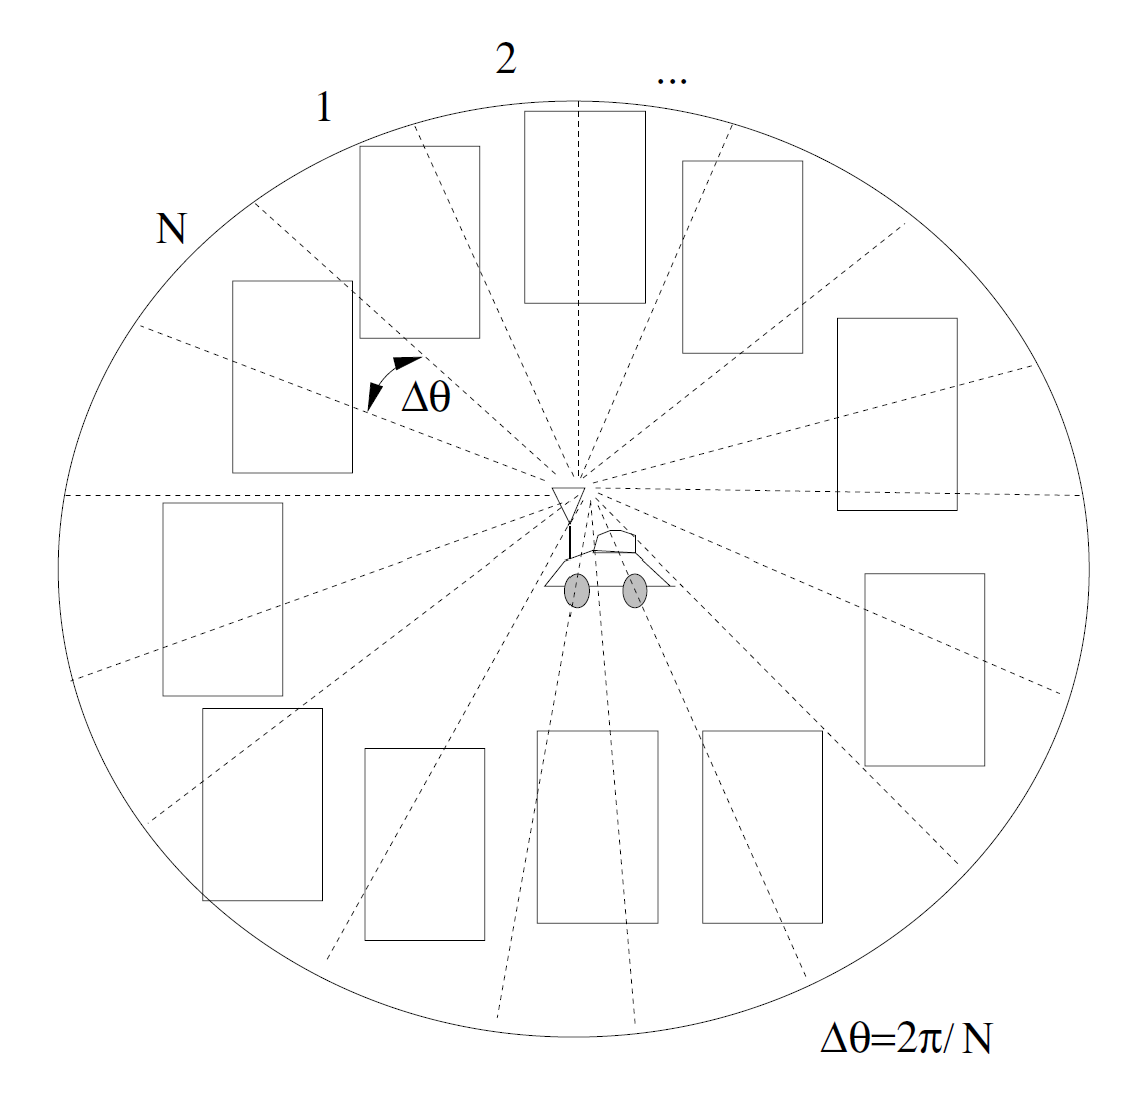
\includegraphics[width=0.6\textwidth]{fig/fig18.png}
		\caption{Uniform \textit{scattering} miljø med jævnt fordelte scatterers}
		\label{fig:uniform_scattering}
	\end{figure}
	
	\[
	A_{r_I}(\tau) = \frac{P_r}{2\pi} \int_0^{2\pi} \cos(2\pi f_D \tau \cos(\theta)) d\theta = P_r J_0(2\pi f_D \tau),
	\]
	
	hvor $P_r$ er den modtagne effekt, og $J_0(2\pi f_D \tau)$ er en Besselfunktion af 0. orden, som beskrevet i Figur \ref{fig:bessel_function}.
	
	\begin{figure}[h!]
		\centering
		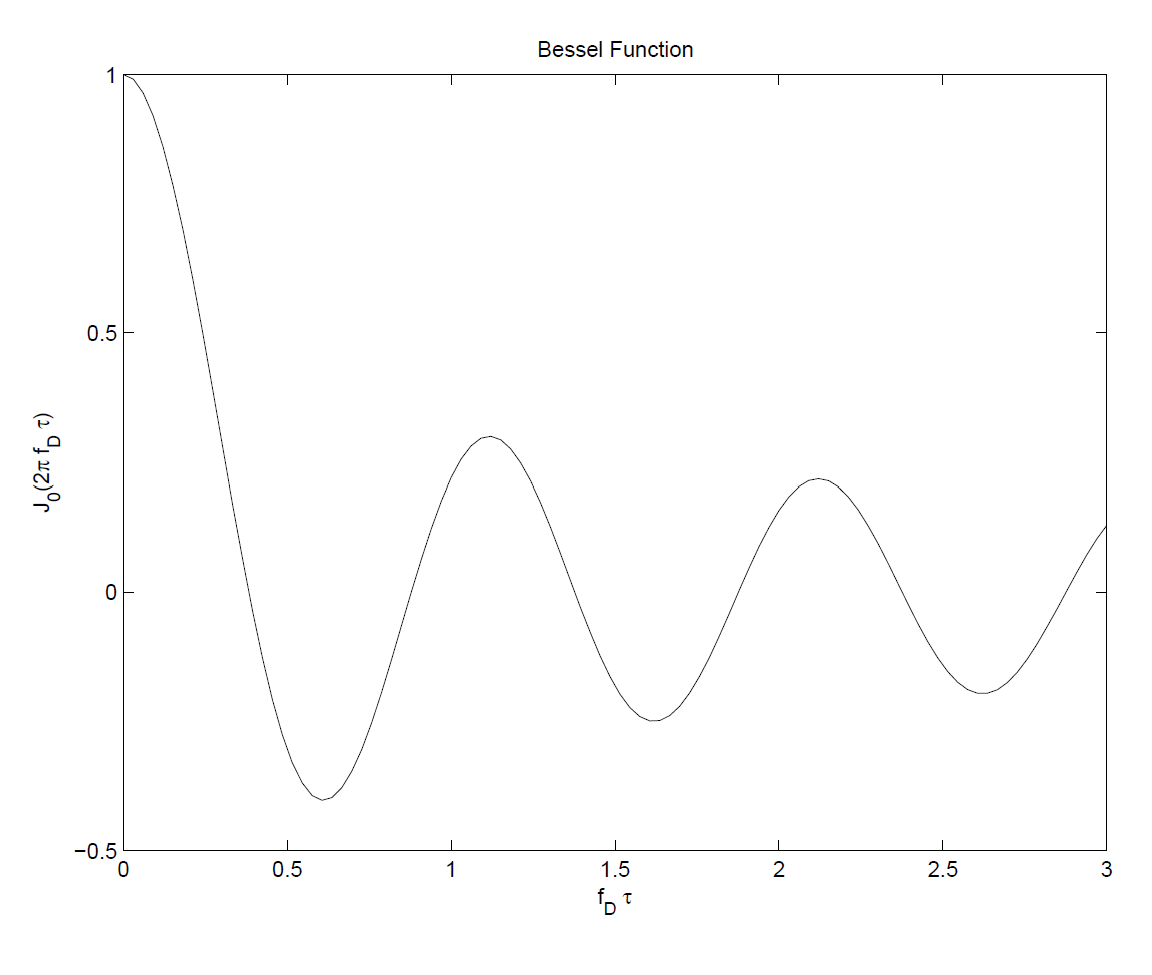
\includegraphics[width=0.5\textwidth]{fig/fig19.png}
		\caption{Bessel-funktion $J_0(2\pi f_D \tau)$ for autokorrelation}
		\label{fig:bessel_function}
	\end{figure}
	
	Denne Besselfunktion beskriver, hvordan autokorrelationen aftager som en funktion af tidsforskellen $\tau$ og Doppler-frekvensen $f_D$.
	
	\subsubsection{Krydskorrelation mellem in-phase og kvadratur komponenter}
	
	Krydskorrelation mellem $r_I(t)$ og $r_Q(t)$ beskriver forholdet mellem de to signaler over tid. Krydskorrelationen er givet ved:
	
	\[
	A_{r_I r_Q}(\tau) = E[r_I(t)r_Q(t + \tau)] = 0,
	\]
	
	da de to komponenter er statistisk uafhængige i dette scenarie. Dette betyder, at der ikke er nogen krydskorrelation mellem de to signaler.
	
	\subsubsection{Spektraltæthed}
	For at beregne spektraltætheden $S_{r_I}(f)$ anvender vi Fourier-transformationen af autokorrelationen:
	
	\[
	S_{r_I}(f) = \mathcal{F}[A_{r_I}(\tau)] = \frac{P_r}{2\pi f_D} \frac{1}{\sqrt{1 - \left(\frac{f}{f_D}\right)^2}} \quad \text{for} \quad |f| \leq f_D.
	\]
	
	Figur \ref{fig:spectrum_density} viser spektraltætheden $S_{r_I}(f)$, som beskriver, hvordan signalets energi er fordelt som funktion af frekvensen.
	\begin{figure}[h!]
		\centering
		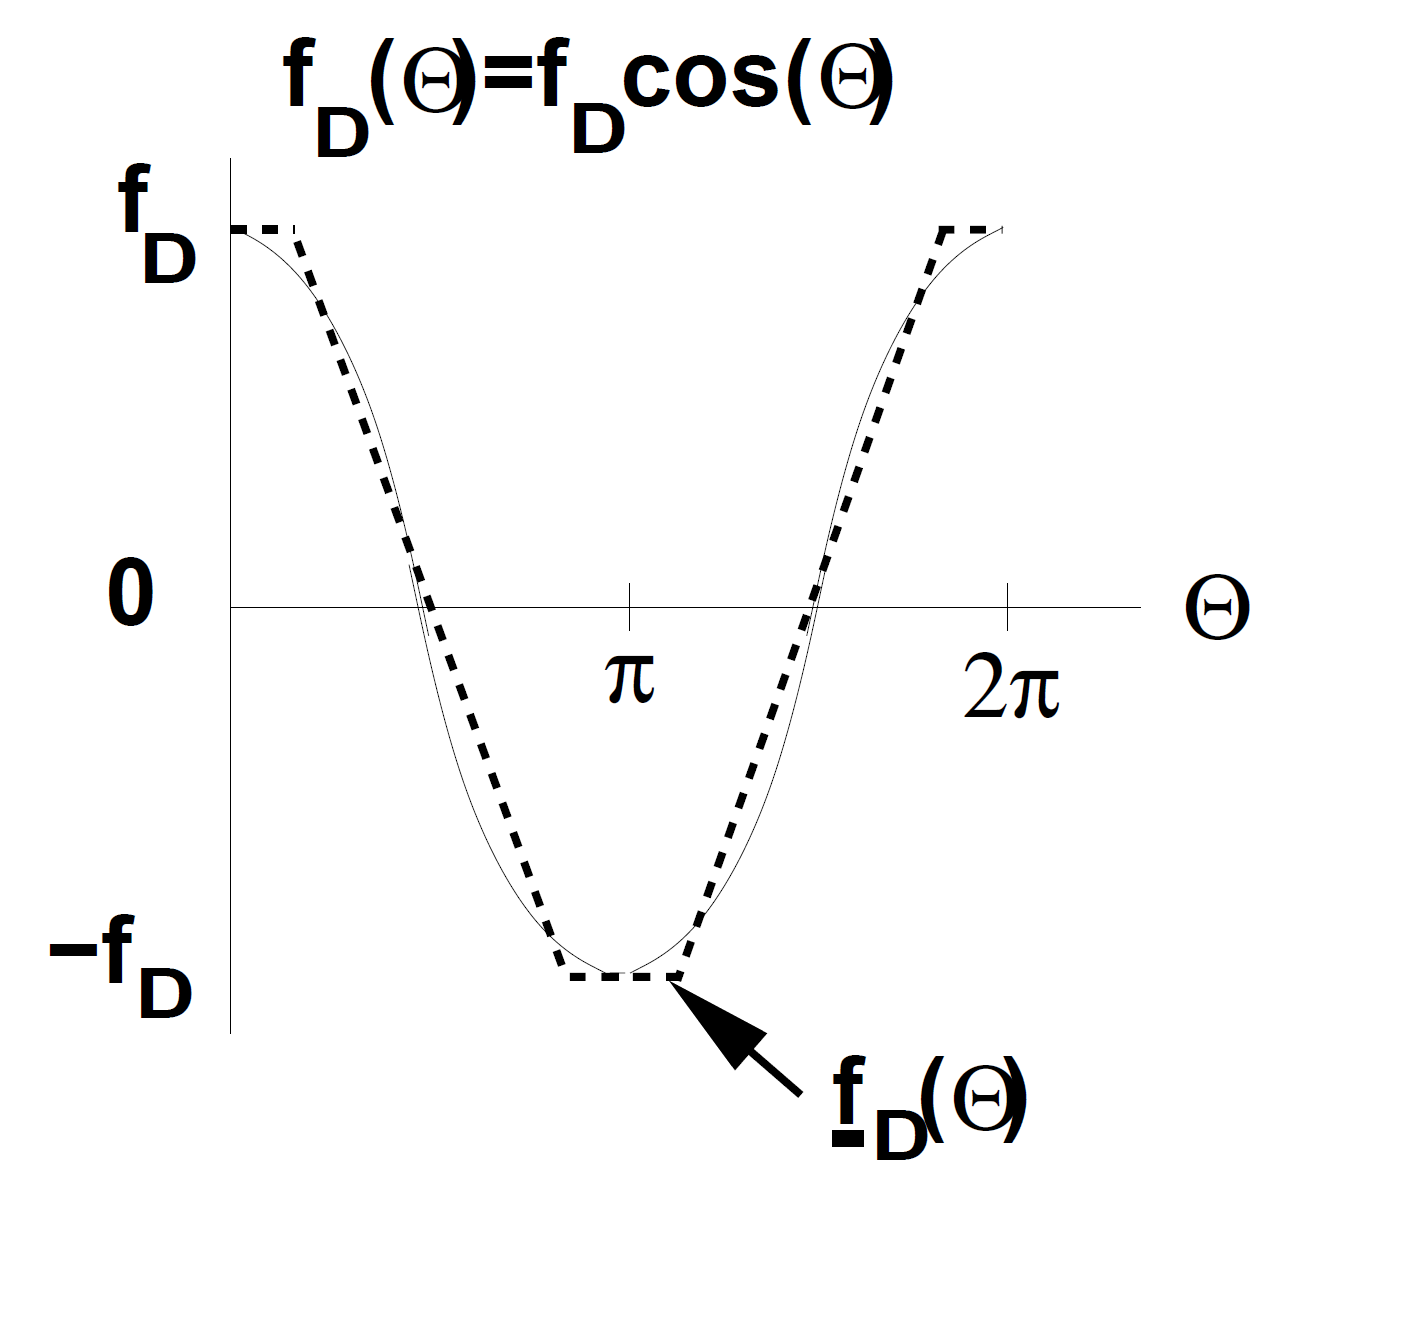
\includegraphics[width=0.4\textwidth]{fig/fig21.png}
		\caption{Spektraltæthed $S_{r_I}(f)$, der viser energifordelingen i signalet}
		\label{fig:spectrum_density}
	\end{figure}
	
	Som vi kan se, er spektraltætheden koncentreret omkring frekvensen $f_D$, og den falder gradvist mod $f = 0$. Denne form beskriver den typiske fordeling af signalets energi over frekvens.
	
	\subsubsection{Doppler-effektens betydning}
	Doppler-effekten opstår som følge af bevægelse mellem sender og modtager, og den ændrer frekvensen af det modtagne signal afhængigt af vinkel $\Theta$. For en uniformt fordelt Doppler-forskydning $f_D(\Theta)$ som funktion af $\Theta$, er Doppler-forskydningen givet ved:
	
	\[
	f_D(\Theta) = f_D \cos(\Theta).
	\]
	\noindent
	Denne relation vises i Figur \ref{fig:doppler_shift}, hvor Doppler-forskydningen når sit maksimum ved $\Theta = 0$ og $\Theta = \pi$, og minimum ved $\Theta = \frac{\pi}{2}$.
	
	\begin{figure}[h!]
		\centering
		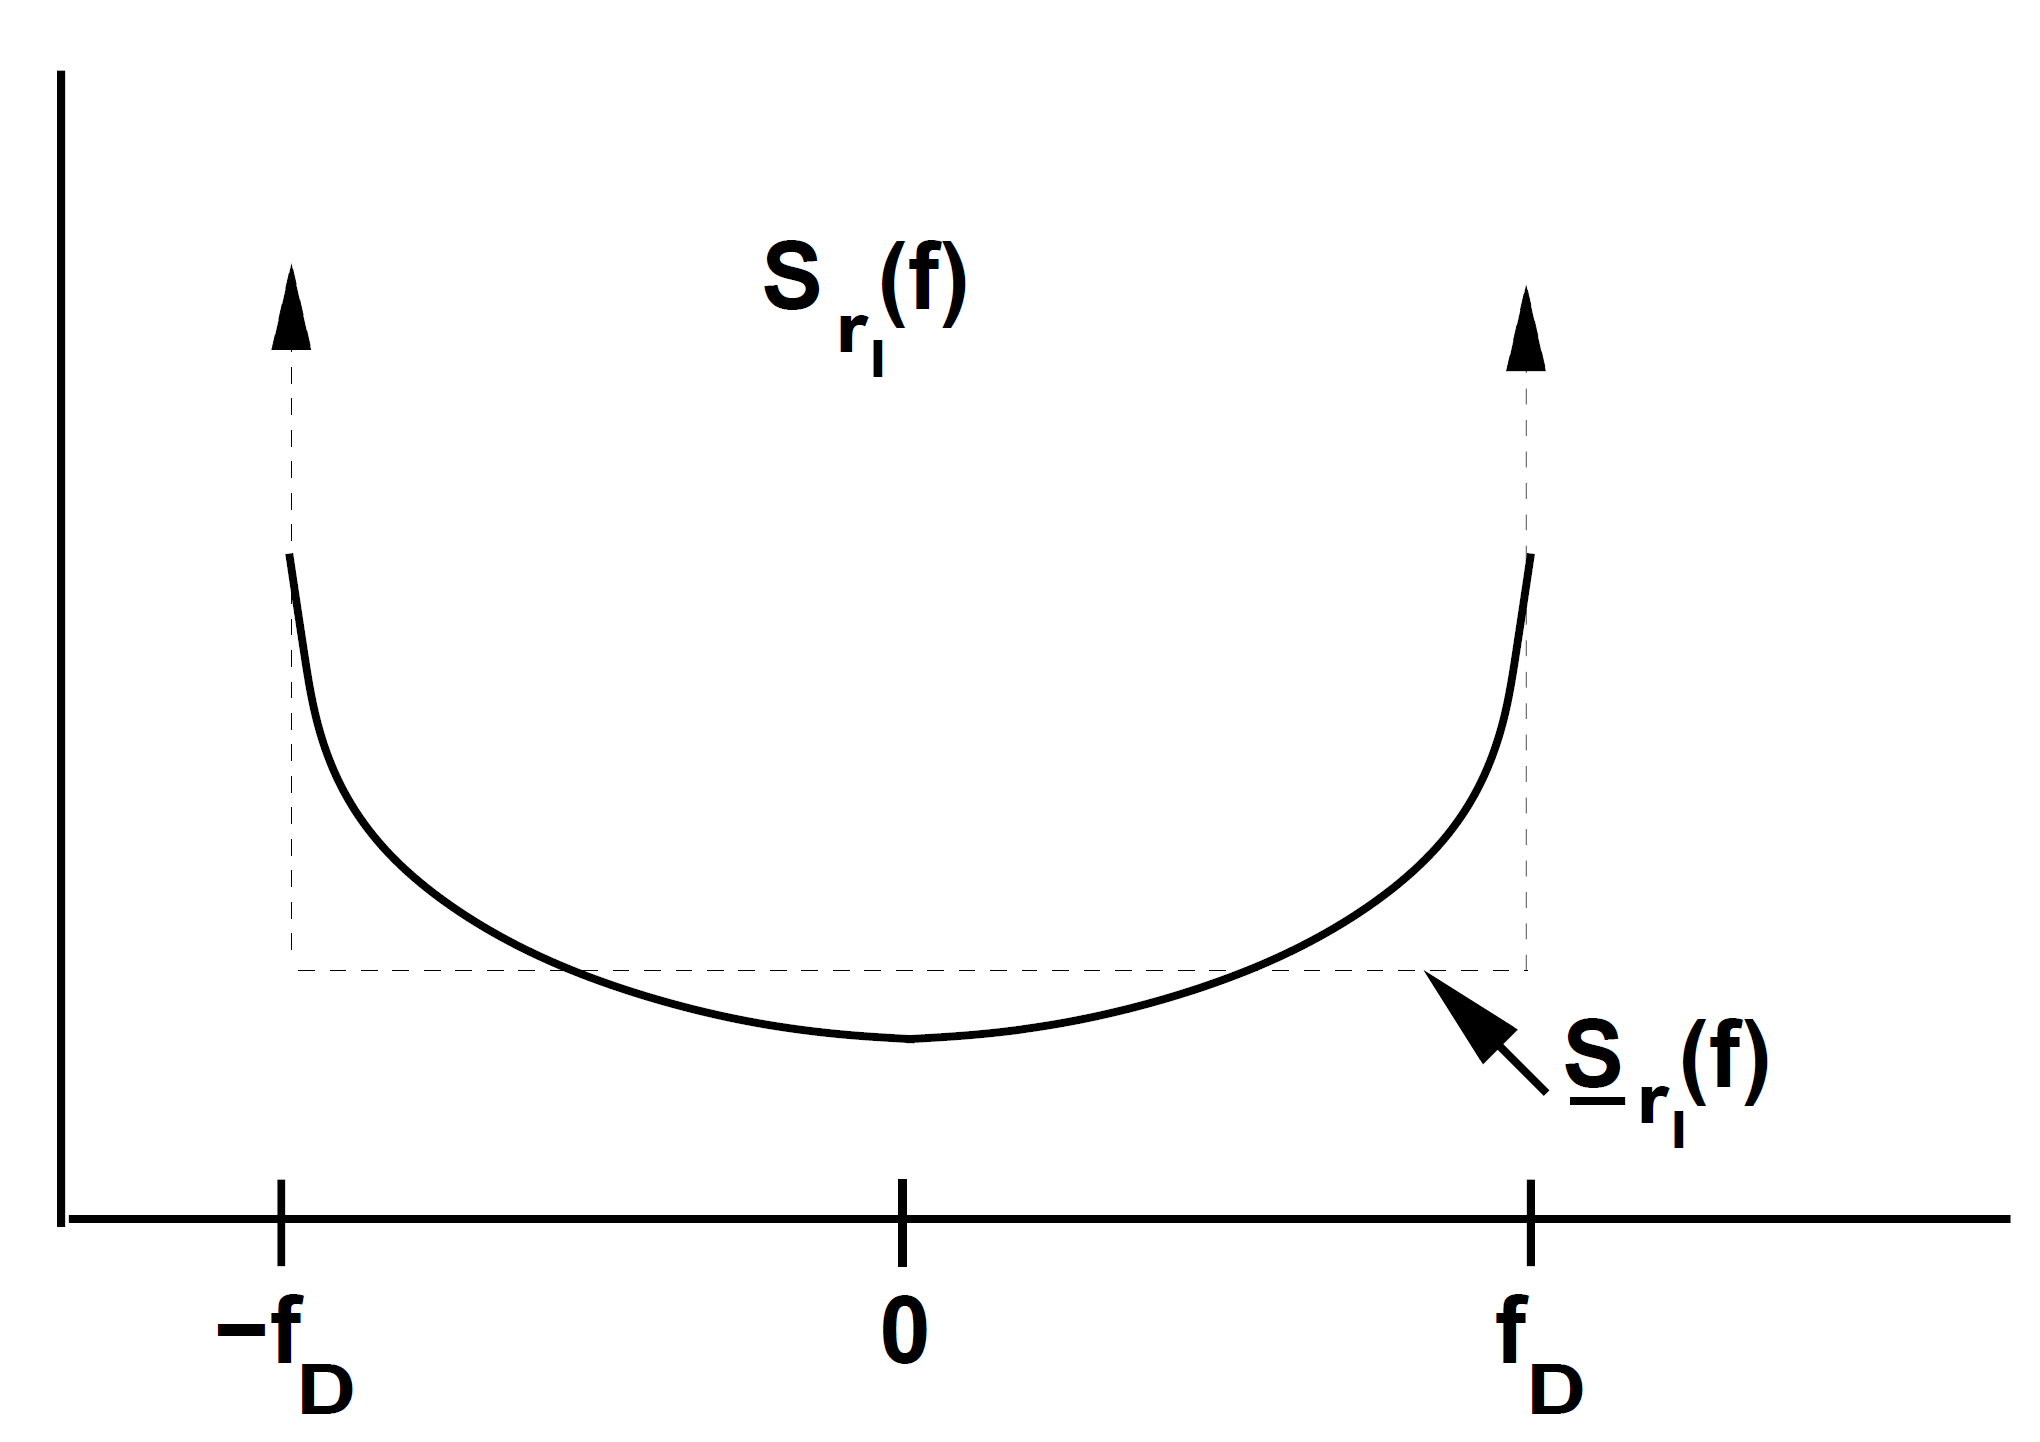
\includegraphics[width=0.4\textwidth]{fig/fig22.png}
		\caption{Doppler-forskydning $f_D(\Theta)$ som en funktion af vinkel $\Theta$}
		\label{fig:doppler_shift}
	\end{figure}
	
	Doppler-effekten har en stor indflydelse på modtagerens signal og skal tages i betragtning ved design af trådløse kommunikationssystemer, især i miljøer med høj bevægelse, som for eksempel køretøjer eller fly.
	
	\section{Envelope and Power Distributions}
	Når vi betragter to tilfældige variabler, $X$ og $Y$, begge med middelværdi nul og varians $\sigma^2$, kan summen af disse, $Z = \sqrt{X^2 + Y^2}$, vise sig at være Rayleigh-fordelt. Kvadratet $Z^2$ vil være eksponentielt fordelt. Tidligere viste vi, at for $\phi_n(t)$, som er uniformt fordelt, er signalets komponenter $r_I$ og $r_Q$ Gaussian-fordelte med nul som middelværdi. Hvis variansen for disse komponenter er $\sigma^2$, kan signalets envelope skrives som:
	
	\[
	z(t) = |r(t)| = \sqrt{r_I^2(t) + r_Q^2(t)}
	\]
	
	Dette udtryk er Rayleigh-fordelt, og sandsynlighedsfordelingen for $z(t)$ er givet ved:
	
	\[
	p_z(z) = \frac{2z}{P_r} \exp\left(-\frac{z^2}{P_r}\right) = \frac{z}{\sigma^2} \exp\left(-\frac{z^2}{2\sigma^2}\right), \quad z \geq 0,
	\]
	
	hvor $P_r$ er den gennemsnitlige modtagne signalstyrke.
	
	\subsection{Rayleigh-fordeling af effekt}
	Effekten i det modtagne signal kan beskrives ved kvadratet af enveloppen $z^2$. Fordelingen af den modtagne effekt er eksponentielt fordelt:
	
	\[
	p_{z^2}(x) = \frac{1}{P_r} \exp\left(-\frac{x}{P_r}\right), \quad x \geq 0.
	\]
	
	Dette viser, at den modtagne signalstyrke har en eksponentiel fordeling med middelværdi $P_r$, hvilket er typisk for Rayleigh fading-kanaler.
	
	\subsection{Eksempel: Rayleigh fading}
	Vi betragter en kanal med Rayleigh fading, hvor den gennemsnitlige modtagne effekt er $P_r = 20$ dBm. Vi ønsker at finde sandsynligheden for, at den modtagne effekt er under 10 dBm.
	
	\[
	p(Z^2 < 10) = \int_0^{10} \frac{1}{100} \exp\left(-\frac{x}{100}\right) dx = 0.095.
	\]
	
	\subsection{Rician fading}
	Hvis vi har en stærk LOS-komponent (Line-of-Sight), vil signalet være en kombination af en Gaussian-fordelt komponent og LOS-komponenten. Envelope i dette tilfælde er Rician-fordelt, givet ved:
	
	\[
	p_z(z) = \frac{z}{\sigma^2} \exp\left( -\frac{z^2 + s^2}{2\sigma^2} \right) I_0\left( \frac{zs}{\sigma^2} \right), \quad z \geq 0,
	\]
	
	hvor $s^2$ er effekten af LOS-komponenten, og $I_0$ er den modificerede Bessel-funktion af 0. orden. Den gennemsnitlige modtagne effekt er:
	
	\[
	P_r = s^2 + 2\sigma^2.
	\]
	
	Rician-fordelingen beskrives ofte med fading-parametret $K$, som er forholdet mellem effekten i LOS-komponenten og multipath-komponenterne:
	
	\[
	K = \frac{s^2}{2\sigma^2}.
	\]
	
	Når $K = 0$, har vi Rayleigh fading, mens højere $K$ indikerer en stærkere LOS-komponent.
	
	\subsection{Nakagami fading}
	Nakagami-fordelingen er en mere generel model, som kan tilpasses mange forskellige miljøer. Nakagami-fordelingen beskrives ved:
	
	\[
	p_z(z) = \frac{2m^m z^{2m-1}}{\Gamma(m) P_r^m} \exp\left( -\frac{mz^2}{P_r} \right), \quad m \geq 0.5,
	\]
	
	hvor $m$ er Nakagami-fadingparameteren. For $m = 1$ reduceres Nakagami til Rayleigh fading, og for $m = \infty$ er der ingen fading.
	
	\begin{figure}[h!]
		\centering
		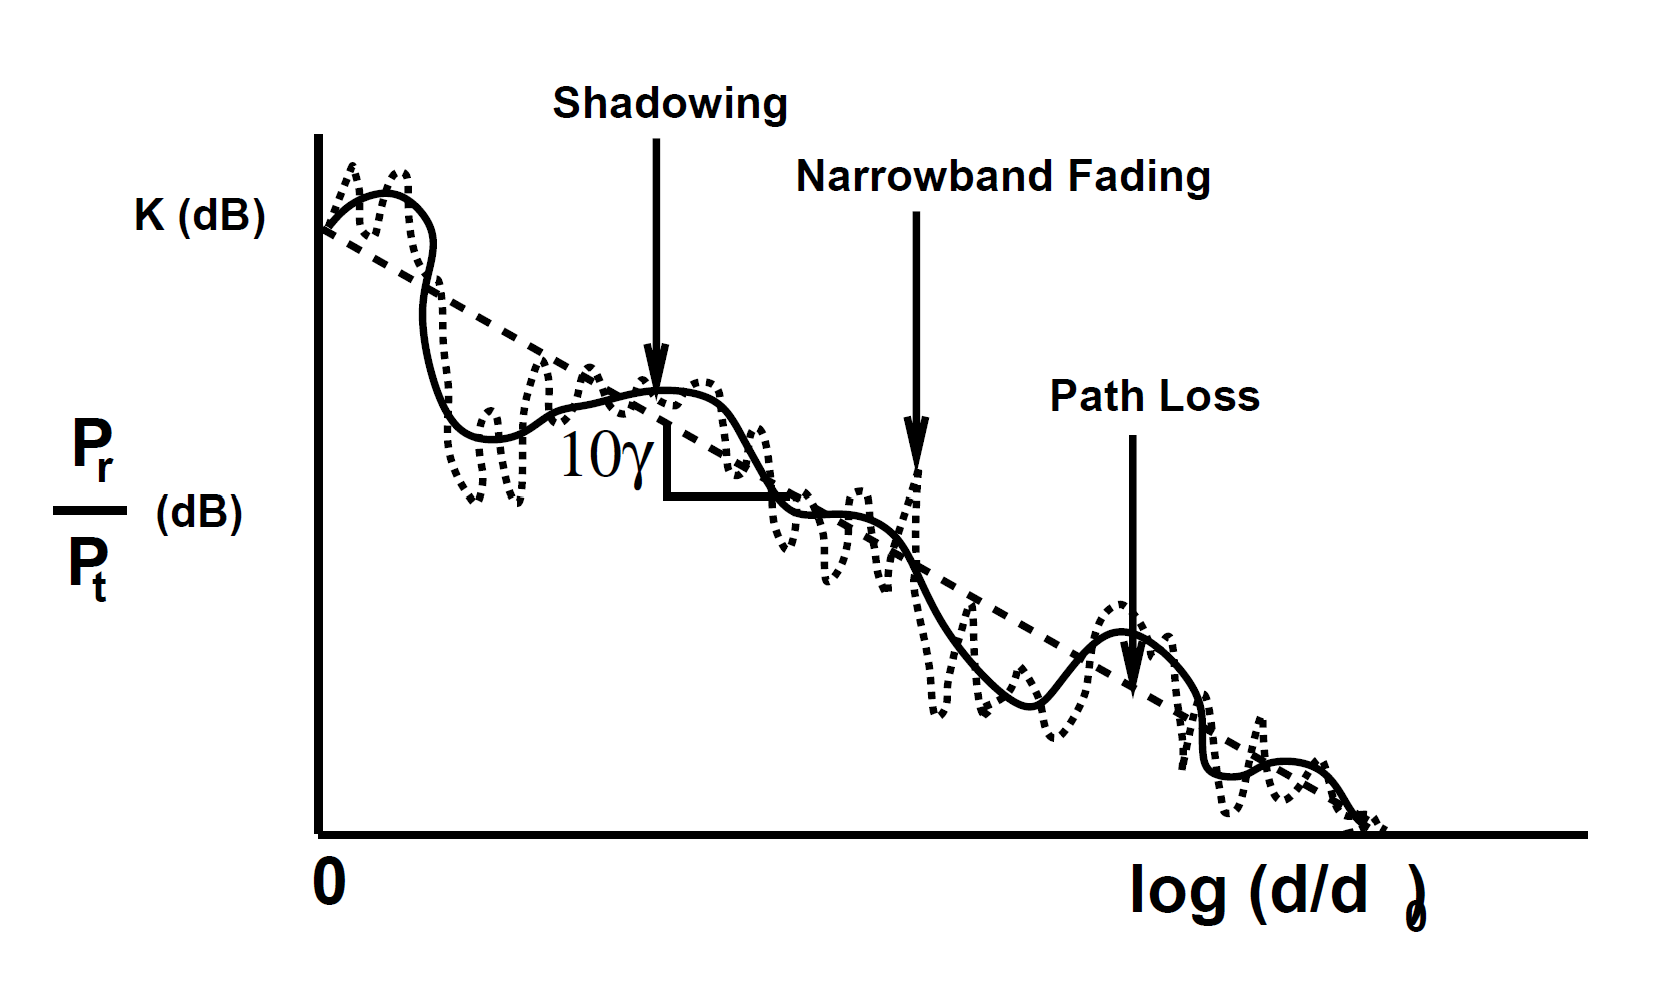
\includegraphics[width=0.6\textwidth]{fig/fig23.png}
		\caption{Kombineret Path Loss, Shadowing og Narrowband Fading.}
	\end{figure}
	
	\begin{figure}[h!]
		\centering
		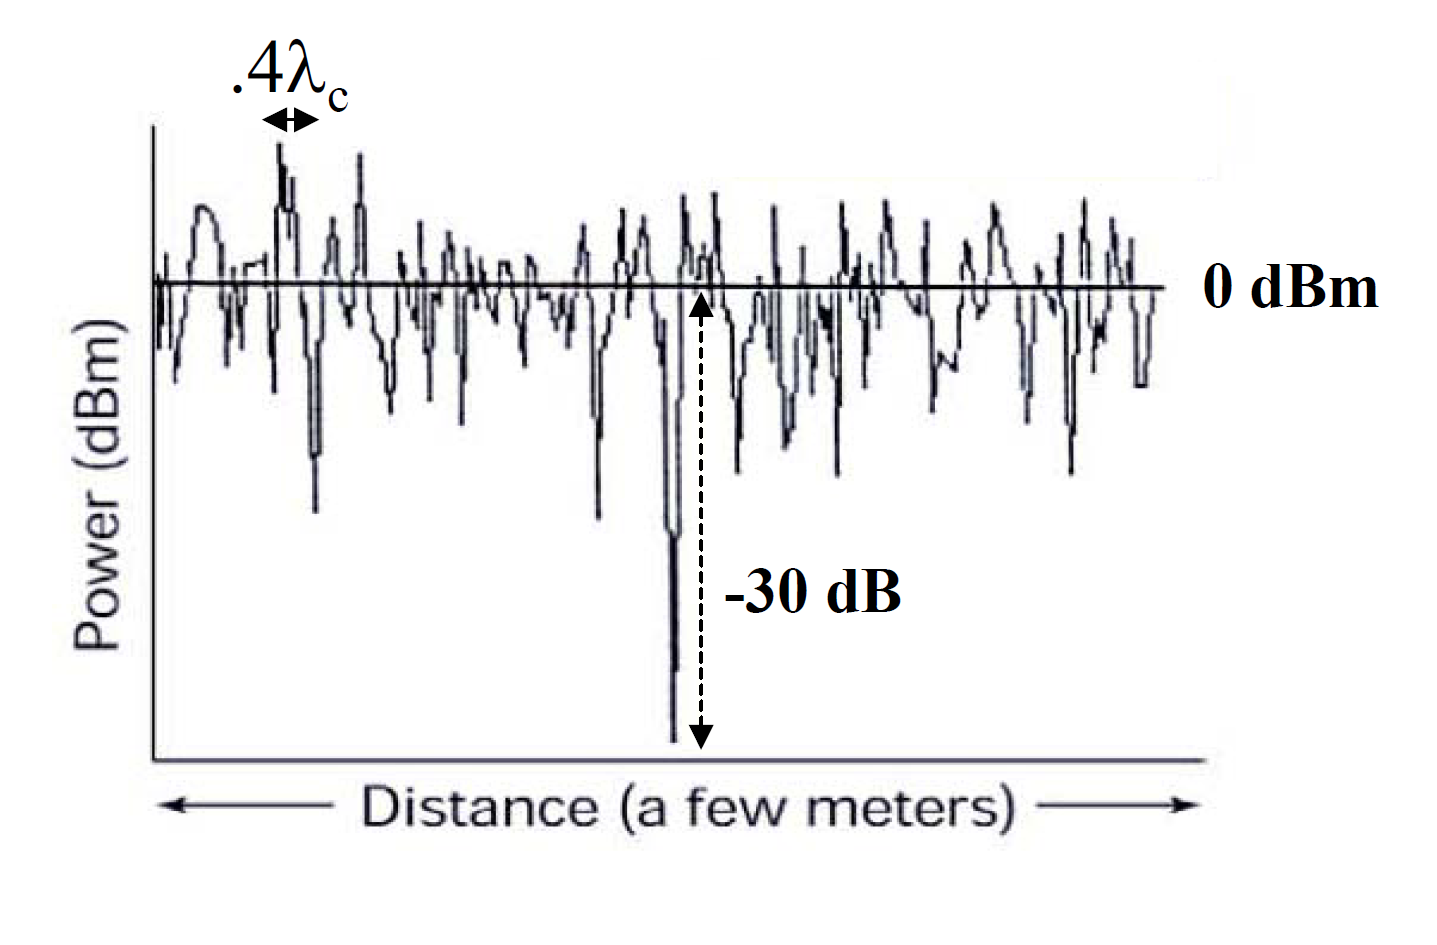
\includegraphics[width=0.6\textwidth]{fig/fig24.png}
		\caption{Narrowband Fading over afstand.}
	\end{figure}
	
	\subsection{Nakagami-fordelingen}
	Den generelle fading-fordeling kaldet Nakagami kan justeres til forskellige målinger, og dens sandsynlighedstæthedsfunktion er givet ved:
	
	\[
	p_Z(z) = \frac{2m^m z^{2m-1}}{\Gamma(m) P_r^m} \exp\left(- \frac{mz^2}{P_r}\right), \quad m \geq 0.5,
	\]
	
	hvor $\Gamma(m)$ er Gamma-funktionen. Nakagami-fordelingen kan modellere både Rayleigh og Rician fading og tilpasses forskellige empiriske observationer.
	
	\[
	p_{Z^2}(x) = \bigg(\frac{m}{P_r}\bigg)^m\frac{x^{m-1}}{\Gamma(m)}exp\bigg(\frac{-mx}{P_r}\bigg).
	\]
	
	\subsection{Level Crossing Rate og Average Fade Duration}
	\textit{Level Crossing Rate (LCR)}, betegnet som $L_Z$, er den forventede hastighed, i krydsninger per sekund, hvormed signalets envelope $z(t) = |r(t)|$ krydser et givet niveau $Z$ i den nedadgående retning. For at udlede $L_Z$ kræves den fælles sandsynlighedsfordeling af signalets envelope $z = |r|$ og dets afledte med hensyn til tid $\dot{z}$, dvs. $p(z, \dot{z})$. Lad os tage udgangspunkt i fading-processen illustreret i figur \ref{fig:level_crossing}, som viser, hvordan envelope $z(t)$ krydser niveauet $Z$ flere gange i en tidsperiode.
	
	\begin{figure}[h]
		\centering
		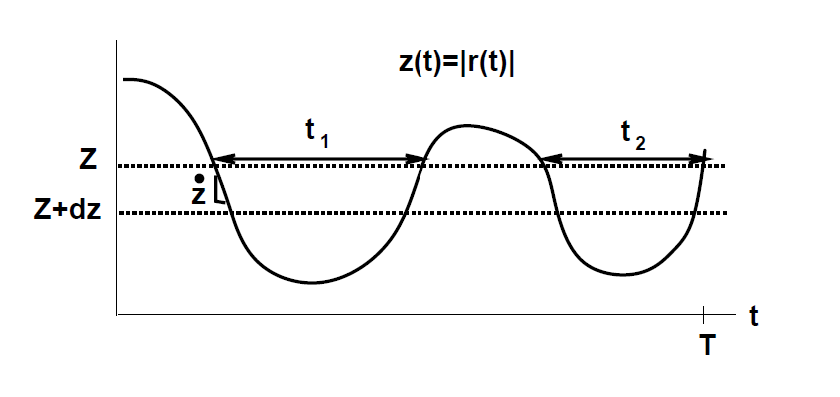
\includegraphics[width=0.5\textwidth]{fig/fig25.png}
		\caption{Level Crossing Rate og Fade Duration for en Fading-proces.}
		\label{fig:level_crossing}
	\end{figure}
	
	For at finde antallet af krydsninger definerer vi først den forventede tid, signalets envelope tilbringer i intervallet $(Z, Z+dz)$ med hældning $\dot{z}$. Dette udtrykkes ved fordelingen $p(Z, \dot{z})d\dot{z}dt$. Krydsningsraten af niveauet $Z$ med negativ hældning over tidsintervallet $[0, T]$ kan udtrykkes som
	
	\[
	L_Z = \int_{-\infty}^{0} \dot{z} p(Z, \dot{z}) d\dot{z}.
	\]
	
	Den forventede tid, hvor signalet $z(t)$ forbliver under niveauet $Z$, betegnes som \textit{Average Fade Duration (AFD)}. AFD, $\bar{t}_Z$, beskriver den gennemsnitlige tid, signalet opholder sig under niveauet $Z$, og kan udledes fra forholdet mellem $L_Z$ og sandsynligheden, $p(z(t) < Z)$, at signalet er under niveauet $Z$:
	
	\[
	p(z(t) < Z) = \frac{1}{T}\sum_{i} t_i,
	\]
	
	hvor $t_i$ er tiden for hvert fade, og $T$ er den samlede tidsperiode. Så den gennemsnitlige fade duration for et stort $T$ er:
	
	\[
	\bar{t}_Z = \frac{1}{T L_Z} \sum_{i=1}^{L_Z T} t_i \approx \frac{p(z(t) < Z)}{L_Z}.
	\]
	
	For Rayleigh fading, hvor $p(z(t) < Z)$ følger Rayleigh-fordelingen, kan vi udtrykke AFD som
	
	\[
	\bar{t}_Z = \frac{e^{\rho^2} - 1}{\rho f_D \sqrt{2\pi}},
	\]
	
	hvor $\rho = Z/\sqrt{P_r}$, $P_r$ er den gennemsnitlige modtagne effekt, og $f_D$ er Doppler-frekvensen.
	
	\subsubsection{Anvendelse af Level Crossing Rate og Average Fade Duration}
	LCR og AFD er vigtige parametre, når man designer trådløse systemer, fordi de giver indikationer på, hvor ofte signalniveauet falder under en bestemt tærskel, samt hvor længe fading varer. For eksempel er disse værdier essentielle for at estimere \textit{bit error rate} (BER) i et kommunikationssystem, da et lavt signalniveau i længere tid kan forårsage mange fejl i signaldekodning.
	
	Eksempel 3.3 viser en anvendelse af disse principper:
	\begin{quote}
		Overvej et stemmesystem med acceptabel \textit{bit error rate (BER)} når det modtagne signal ligger over halvdelen af dets gennemsnitlige værdi. Find området af Doppler-værdier, der sikrer, at stemmekvaliteten er acceptabel i et Rayleigh fading miljø, hvor brugere oplever en dårlig kvalitet i mindre end $t = 60$ ms. Løsningen er at bruge formlen for AFD og løse for $f_D$:
		\[
		f_D \geq \frac{e^{5} - 1}{(.060\sqrt{2\pi})} \approx 6.1 \text{ Hz}.
		\]
	\end{quote}
	
	Dette betyder, at Doppler-frekvensen skal være mindst $6.1$ Hz for at opretholde en acceptabel stemmekvalitet i en Rayleigh fading kanal, hvor signalniveauet ofte krydser tærsklen på halvdelen af den gennemsnitlige signalstyrke.
	
	
	\subsection{Finite State Markov Channels (FSMC)}
	\label{sec:fsmc}
	
	I trådløse kommunikationssystemer er fading en uundgåelig effekt, der kan påvirke signaloverførslen negativt. For at modellere og analysere fading-kanaler anvendes ofte en Finite State Markov Channel (FSMC)-model. FSMC-modellen tilnærmer fading-processen ved at diskretisere den kontinuerlige tid i en række tidsintervaller, typisk valgt svarende til symbolperioden \(T_s\).
	
	\subsubsection{Tilstande i FSMC}
	FSMC-modellen deler signalets signal-til-støj-forhold (SNR) op i et endeligt antal regioner, kaldet tilstande. Hver region repræsenterer et bestemt interval af SNR. For en kanal, der påvirkes af \textit{Rayleigh} fading, ligger SNR \( \gamma \) i intervallet \( 0 \leq \gamma \leq \infty \). Regionerne \( R_j \) defineres som:
	\[
	R_j = \{ A_j \leq \gamma < A_{j+1} \},
	\]
	hvor \( A_j \) og \( A_{j+1} \) er grænseværdierne for regionen \(R_j\). Hver region kan betragtes som en diskret tilstand i FSMC-modellen. Over tid vil kanalen skifte mellem disse tilstande baseret på sandsynligheder, der afhænger af kanalens fysiske parametre, såsom Doppler-forskydning og symbolperioden \( T_s \).
	
	\subsubsection{Markov-egenskaber}
	FSMC-modellen antager, at kanalen i hvert tidsinterval forbliver i én af de diskrete tilstande og kun kan skifte til tilstanden før eller efter i den næste tidsperiode. Overgangen mellem tilstandene bestemmes af Markov-egenskaber, hvor sandsynligheden for at skifte fra en tilstand til en anden kun afhænger af den nuværende tilstand, ikke af tidligere tilstande.
	
	Overgangssandsynlighederne kan beregnes ved hjælp af følgende ligninger:
	\[
	p_{j,j+1} = \frac{N_j T_s}{\pi_j}, \quad p_{j,j-1} = \frac{N_j T_s}{\pi_j}, \quad p_{j,j} = 1 - p_{j,j+1} - p_{j,j-1},
	\]
	hvor:
	\begin{itemize}
		\item \( N_j \) er antal krydsninger af niveau \( A_j \) pr. sekund (level-crossing rate).
		\item \( \pi_j \) er steady-state sandsynlighedsfordelingen for at være i region \( R_j \), givet ved \( \pi_j = P(\gamma \in R_j) = P(A_j \leq \gamma < A_{j+1}) \).
	\end{itemize}
	
	\subsubsection{Anvendelse af FSMC}
	FSMC-modeller er nyttige til at forenkle den komplekse karakter af fading, især for analytisk beregning af fejlrate (Packet Error Rate, PER) og systemperformance. Modellen bruges bredt til at beskrive både Rayleigh og Ricean fading-kanaler, samt mere generelle fading-modeller såsom Nakagami-\(m\) fading.
	
	\subsubsection{Fordele ved FSMC-modellen}
	FSMC-modellen gør det muligt at reducere komplekse kanalanalyser til simple diskrete overgange mellem tilstande. Dette gør det muligt at foretage præcise analyser af systemer, der oplever fading, og hjælpe med at estimere, hvordan fading vil påvirke f.eks. signalkvaliteten eller fejlrate.
	
	\subsubsection{Eksempel: FSMC for Rayleigh Fading}
	For en Rayleigh fading-kanal kan SNR-værdien \( \gamma \) variere hurtigt mellem regionerne \( R_j \), som beskrevet ovenfor. Ved brug af FSMC-modellen kan overgangssandsynlighederne mellem forskellige tilstande bestemmes og bruges til at modellere kanalens adfærd over tid. Dette kan være særligt nyttigt til at estimere, hvor ofte systemet vil opleve fading-dips, hvilket kan påvirke systemets præstation.
	
	\section{Wideband Fading Models}
	Når signalet ikke er smalbåndet, opstår der en anden form for forvrængning på grund af \textit{multipath delay spread}. Et kort transmitteret signal med varighed $T$ vil resultere i et modtaget signal, der har en varighed på $T + T_m$, hvor $T_m$ er \textit{multipath delay spread}. Dette medfører, at det modtagne signal vil være betydeligt forvrænget. Som illustreret i Figur 3.11, hvis $T$ transmitteres over en \textit{multipath channel}, kan multipath-komponenterne, der ankommer med forskellig forsinkelse $\tau_n$, føre til interferens.
	
	\begin{figure}[h]
		\centering
		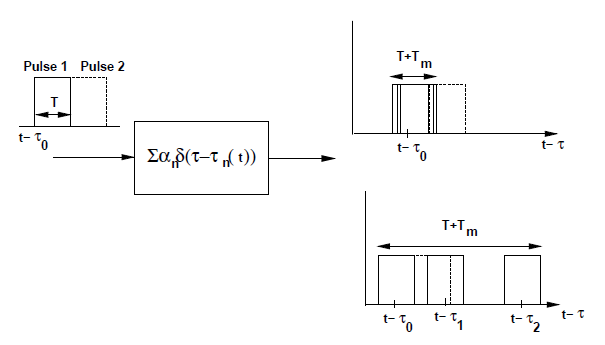
\includegraphics[width=0.7\textwidth]{fig/fig26.png}
		\caption{Multipath Resolution.}
	\end{figure}
	
	Hvis \textit{multipath delay spread} er lille, det vil sige $T_m \ll T$, ankommer multipath-komponenterne næsten samtidigt og interfererer konstruktivt og destruktivt, hvilket fører til smalbånds \textit{fading}. I dette tilfælde er der minimal spredning i tid af de forskellige \textit{multipath} komponenter, og signalforvrængningen er lav.
	\newline\newline
	På den anden side, hvis \textit{multipath delay spread} er stort, $T_m \gg T$, kan de forskellige komponenter adskilles, hvilket giver mulighed for tidsmæssig opløsning af de forskellige refleksioner (multipath-komponenter), som vist på Figur 3.12. Dette kan dog føre til \textit{intersymbol interference (ISI)} mellem efterfølgende transmitterede symboler. Dette problem opstår, fordi tidligere refleksioner interfererer med efterfølgende symboler. \textit{ISI} er ofte uønsket i kommunikationssystemer, da det kan påvirke modtagelseskvaliteten.
	
	\begin{figure}[h]
		\centering
		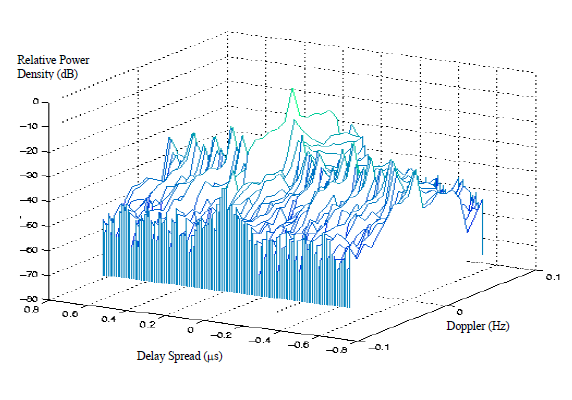
\includegraphics[width=0.7\textwidth]{fig/fig27.png}
		\caption{Scattering Function.}
	\end{figure}
	
	En vigtig faktor i bredbåndskanaler er karakteriseringen af den tilsvarende lavpas kanalimpulsrespons $c(\tau,t)$. Denne karakterisering kan udføres ved at tage Fourier-transformationen af $c(\tau,t)$ for at få spredningsfunktionen $S_c(\tau, \rho)$, som er givet ved:
	
	\[
	S_c(\tau, \rho) = \int_{-\infty}^{\infty} c(\tau, t)e^{-j2\pi \rho t} dt
	\]
	
	hvor $\rho$ er Doppler-frekvensen. Denne spredningsfunktion viser, hvordan kanalens output er relateret til både \textit{multipath delay} og Doppler-spredning. Figur 3.12 viser et eksempel på en typisk spredningsfunktion, hvor man kan se sammenhængen mellem forsinkelse og Dopplerforskydning.
	\newline\newline
	I bredbåndskanaler, som vi ser her, spiller \textit{multipath delay spread} og \textit{Doppler spread} en afgørende rolle i forvrængningen af signalet. Forsinkelsen mellem de forskellige refleksioner kan forårsage \textit{fading}, og Doppler-spredningen introducerer frekvensafvigelser, der påvirker signalets fase og amplitude over tid.
	
	\subsection{Matematisk Modellering}
	For at modellere de nævnte fænomener kan vi se på den statistiske karakterisering af $c(\tau,t)$ via autokorrelationsfunktionen:
	
	\[
	A_c(\tau_1, \tau_2; \Delta t) = E[c^*(\tau_1; t)c(\tau_2; t+\Delta t)]
	\]
	
	I praksis antages det, at kanalen er bredbåndsstationær (WSS), hvilket betyder, at autokorrelationsfunktionen kun afhænger af tidsforskellen $\Delta t$ og ikke af $t$ direkte:
	
	\[
	A_c(\tau_1, \tau_2) = E[c^*(\tau_1)c(\tau_2)].
	\]
	
	Den tidsvarierende kanalimpulsrespons og dens Doppler-komponenter kan derfor bruges til at beskrive de randomiserede ændringer i signalet over tid.
	\newline\newline
	I bredbåndskanaler er det vigtigt at tage hensyn til både \textit{multipath delay spread} og \textit{Doppler spread} for at karakterisere signalforvrængningen. Forskellige teknikker, som f.eks. \textit{equalization} og \textit{multicarrier modulation}, kan bruges til at afhjælpe problemerne med \textit{intersymbol interference (ISI)} og forbedre systemets ydeevne i bredbåndsmiljøer.
	
	\subsection{Power Delay Profile}
	\label{sec:power_delay_profile}

	Power Delay Profile (PDP) beskriver, hvordan den modtagne effekt fordeler sig over tid fra forskellige multipath-komponenter, som signalet har bevæget sig gennem på vej fra senderen til modtageren. PDP'en er vigtig, fordi den hjælper os med at forstå forsinkelserne af signaler i et trådløst miljø og deres effekt på kommunikationssystemer.
	
	Den matematiske definition af PDP er relateret til kanalens impulssvar \( h(t, \tau) \). PDP'en \( P_h(\tau) \) er givet ved:
	
	\[
	P_h(\tau) = \lim_{T \to \infty} \frac{1}{2T} \int_{-T}^{T} |h(t, \tau)|^2 \, dt
	\]
	
	Denne ligning betyder, at PDP'en viser, hvordan energien i signalet varierer som funktion af forsinkelsen \( \tau \) for multipath-komponenterne.
	
	For at forstå signalets forsinkelse over tid, kan vi beregne den **gennemsnitlige forsinkelse** \( T_m \), som er det første moment af PDP'en:
	
	\[
	T_m = \frac{\int_{-\infty}^{\infty} P_h(\tau) \tau \, d\tau}{\int_{-\infty}^{\infty} P_h(\tau) \, d\tau}
	\]
	
	Dette udtryk giver en idé om, hvor lang tid signalet i gennemsnit forsinkes i forhold til den direkte signalvej.
	
	En anden vigtig parameter er **root mean square (rms) forsinkelsesspredningen** \( S_{\tau} \), som måler spredningen af forsinkelserne omkring den gennemsnitlige forsinkelse \( T_m \). Den defineres som:
	
	\[
	S_{\tau} = \sqrt{\frac{\int_{-\infty}^{\infty} P_h(\tau) \tau^2 \, d\tau}{\int_{-\infty}^{\infty} P_h(\tau) \, d\tau} - T_m^2}
	\]
	
	Denne størrelse fortæller, hvor meget multipath-forsinkelserne varierer. Det er en vigtig faktor, når man skal beregne risikoen for **intersymbolinterferens (ISI)**, som opstår, når signaler overlapper hinanden, hvis symbolperioden \( T_s \) er for lille i forhold til \( S_{\tau} \).
	
	For at undgå ISI skal vi sikre, at symbolperioden \( T_s \) er større end rms forsinkelsesspredningen:
	
	\[
	T_s > S_{\tau}
	\]
	
	Når du arbejder med PDP i opgaver, skal du typisk beregne \( T_m \) og \( S_{\tau} \) for at forstå, hvordan signalerne forstyrres af multipath-effekter, og hvordan systemet kan kompensere for dem.
	
	\subsubsection{Eksempel:}
	Effektspektrummet for forsinkelse modelleres ofte som en ensidet eksponentiel fordeling:
	
	\[
	A_c(\tau) = \frac{1}{T_m} e^{-\tau/T_m}, \quad \tau \geq 0.
	\]
	
	Vis, at den gennemsnitlige forsinkelsesspredning er \( \mu_{T_m} = T_m \), og find RMS forsinkelsesspredningen \( \sigma_{T_m} \).
	\newline\newline
	\textbf{Løsning:} Det er let at vise, at \( A_c(\tau) \) integreres til én. Den gennemsnitlige forsinkelsesspredning er derfor givet ved
	
	\[
	\mu_{T_m} = \frac{1}{T_m} \int_0^\infty \tau e^{-\tau/T_m} d\tau = T_m.
	\]
	
	RMS forsinkelsesspredningen \( \sigma_{T_m} \) er:
	
	\[
	\sigma_{T_m} = \sqrt{\frac{1}{T_m} \int_0^\infty \tau^2 e^{-\tau/T_m} d\tau - \mu_{T_m}^2} = \sqrt{2T_m^2 - T_m^2} = T_m.
	\]
	
	Således er den gennemsnitlige og RMS forsinkelsesspredning de samme for eksponentielt fordelte effektspektrummer for forsinkelse.
	
	\subsubsection{Eksempel:}
	Overvej en bredbåndskanal med multipath intensitetsprofil
	
	\[
	A_c(\tau) = 
	\begin{cases} 
		e^{-\tau / .00001}, & 0 \leq \tau \leq 20 \, \mu s, \\
		0, & \text{ellers}.
	\end{cases}
	\]
	
	Find den gennemsnitlige og RMS forsinkelsesspredning for kanalen, og find den maksimale symbolrate, sådan at et lineært moduleret signal, der transmitteres gennem denne kanal, ikke oplever ISI.
	\newline\newline
	\textbf{Løsning:} Den gennemsnitlige forsinkelsesspredning er:
	
	\[
	\mu_{T_m} = \frac{\int_0^{20 \cdot 10^{-6}} \tau e^{-\tau / .00001} d\tau}{\int_0^{20 \cdot 10^{-6}} e^{-\tau / .00001} d\tau} = 6.87 \, \mu s.
	\]
	
	RMS forsinkelsesspredningen er:
	
	\[
	\sigma_{T_m} = \sqrt{\frac{\int_0^{20 \cdot 10^{-6}} (\tau - \mu_{T_m})^2 e^{-\tau / .00001} d\tau}{\int_0^{20 \cdot 10^{-6}} e^{-\tau / .00001} d\tau}} = 5.25 \, \mu s.
	\]
	
	Vi ser i dette eksempel, at den gennemsnitlige forsinkelsesspredning er omtrent lig med RMS-værdien. For at undgå ISI skal symbolperioden \( T_s \) være større end \( 10\sigma_{T_m} \). Dette betyder, at \( T_s > 10 \cdot 5.25 \, \mu s = 52.5 \, \mu s \), hvilket giver en symbolrate på \( R_s = 1 / T_s = 19.04 \, \text{Ksymb/s} \). Dette er en stærkt begrænset symbolrate for mange trådløse systemer.
	
	
	\subsection{Coherence Bandwidth}
	\textbf{Coherence Bandwidth (Sammenhængende båndbredde)} er et vigtigt koncept i analyse af trådløse kommunikationskanaler, da det beskriver det frekvensområde, hvor kanalens egenskaber forbliver korrelerede. Dette betyder, at signaler, der ligger inden for denne båndbredde, vil opleve lignende fading-karakteristika, og dermed kan man undgå frekvensselektiv fading.
	\newline\newline
	Sammenhængende båndbredde er tæt relateret til kanalens tidsmæssige karakteristika, specielt kanalens forsinkelsesspredning. Den sammenhængende båndbredde \( B_c \) kan defineres som det frekvensområde, hvor signaler forbliver korrelerede. Matematikken bag dette bygger på kanalens frekvenskorrelationsfunktion \( A_C(f_1, f_2; \Delta t) \), som beskriver korrelationen mellem fading ved to forskellige frekvenser \( f_1 \) og \( f_2 \):
	
	\[
	A_C(f_1, f_2; \Delta t) = \mathbb{E}[C^*(f_1; t) C(f_2; t + \Delta t)].
	\]
	
	Hvor \( C(f; t) \) er defineret som:
	
	\[
	C(f; t) = \int_{-\infty}^{\infty} c(\tau; t) e^{-j 2 \pi f \tau} d\tau.
	\]
	
	Udtrykket for frekvenskorrelationsfunktionen kan yderligere udvides til:
	
	\[
	A_C(f_1, f_2; \Delta t) = \int_{-\infty}^{\infty} A_c(\tau, \Delta t) e^{-j 2 \pi (f_2 - f_1) \tau} d\tau,
	\]
	
	hvor \( A_c(\tau) \) er kanalens tidsmæssige korrelationsfunktion. For tilfældet af to frekvenser \( f_1 \) og \( f_2 \) med en forskel \( \Delta f = f_2 - f_1 \), reduceres udtrykket til:
	
	\[
	A_C(\Delta f) = \int_{-\infty}^{\infty} A_c(\tau) e^{-j 2 \pi \Delta f \tau} d\tau.
	\]
	
	Dette viser, at den sammenhængende båndbredde \( B_c \) kan tolkes som det område i frekvensdomænet, hvor korrelationsfunktionen forbliver signifikant, som illustreret i figuren nedenfor:
	
	\begin{figure}[!h]
		\centering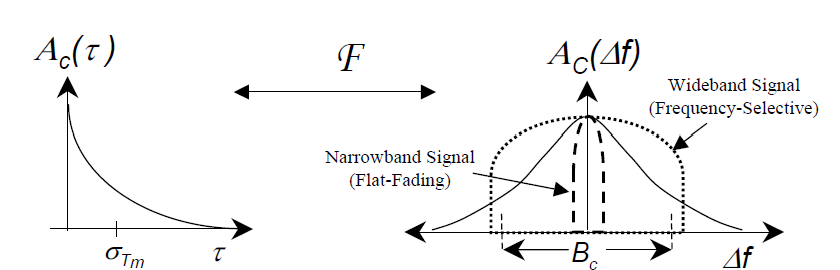
\includegraphics[width=\textwidth]{fig/fig28.png}
		\caption{Power Delay Profile, RMS Delay Spread, and Coherence Bandwidth.}
	\end{figure}
	
	I figuren ses \( A_c(\tau) \) som kanalens tidsmæssige korrelation, der er relateret til kanalens forsinkelsesspredning \( \sigma_{T_m} \). Den Fourier-transformerede funktion \( A_C(\Delta f) \) beskriver korrelationen i frekvensdomænet, hvor den sammenhængende båndbredde \( B_c \) angiver det interval, inden for hvilket kanalen opfører sig som en smalbåndskanal med flad fading. Uden for dette interval opleves frekvensselektiv fading, som har større variation over frekvens.
	\newline\newline
	Når signalets båndbredde \( B \) er meget mindre end \( B_c \), er fading flad over hele båndbredden, hvilket er typisk for smalbåndssignaler. Men hvis \( B \) er større end \( B_c \), oplever vi frekvensselektiv fading, hvor forskellige frekvenskomponenter påvirkes forskelligt af kanalen.
	\newline\newline
	I praksis skal symbolperioden \( T_s \) være større end den inverse af den sammenhængende båndbredde \( B_c \) for at undgå interferens mellem symboler (ISI). Dette kan udtrykkes som:
	
	\[
	T_s > \frac{1}{B_c}.
	\]
	
	Sammenhængende båndbredde er derfor en essentiel parameter for at bestemme, om en kommunikationskanal oplever flad eller frekvensselektiv fading, hvilket har stor betydning for valg af modulationsteknik og systemdesign.
	
	\subsubsection{Eksempel:}
	For en kanal med Doppler-spredning \( B_d = 80 \, \text{Hz} \), hvilken tidsadskillelse kræves mellem prøver af det modtagne signal, så prøverne er tilnærmelsesvis uafhængige?
	\newline\newline
	\textbf{Løsning:} Sammenhængstiden for kanalen er \( T_c \approx 1 / B_d = 1 / 80 \), så prøver, der er adskilt med 12.5 ms, er tilnærmelsesvis ukorrelerede. Givet de Gaussiske egenskaber af den underliggende stokastiske proces er disse prøver derfor tilnærmelsesvis uafhængige.
	
	\subsection{Doppler Power Spectrum and Channel Coherence Time}
	\subsection*{Transforms for Autocorrelation and Scattering Functions}
	I trådløse kanaler spiller både autokorrelationsfunktionen \( A_c(\tau, \Delta t) \) og spredningsfunktionen \( S_c(\tau, \rho) \) en central rolle i analysen af kanalen. Disse funktioner er tæt forbundet gennem Fourier-transformationer.
	\newline\newline
	Den dobbelte Fourier-transformation mellem \( A_c(\Delta f, \Delta t) \) og \( S_c(\tau, \rho) \) kan beskrives som:
	
	\[
	S_c(\tau, \rho) = \int_{-\infty}^{\infty} \int_{-\infty}^{\infty} A_c(\Delta f, \Delta t) e^{-j 2 \pi \rho \Delta t} e^{j 2 \pi \tau \Delta f} d\Delta t d\Delta f.
	\]
	
	Denne ligning viser sammenhængen mellem spredningsfunktionen \( S_c(\tau, \rho) \) og autokorrelationsfunktionen \( A_c(\Delta f, \Delta t) \) gennem en dobbelt Fourier-transformation.
	
	\[
	A_c(\Delta f, \Delta t) = \int_{-\infty}^{\infty} \int_{-\infty}^{\infty} S_c(\tau, \rho) e^{j 2 \pi \Delta f \tau} e^{-j 2 \pi \rho \Delta t} d\tau d\rho.
	\]
	
	Autokorrelations- og spredningsfunktionerne er dermed relateret på følgende måde:
	
	\begin{itemize}
		\item \( A_c(\tau, \Delta t) \) er den inverse Fourier-transformation af \( S_c(\tau, \rho) \) i Doppler-domænet \( \rho \).
	
		\item \( S_c(\Delta f, \rho) \) er Fourier-transformen af \( A_c(\Delta f, \Delta t) \) i både frekvens- og tidsdomenet.
	\end{itemize}
	
	Figuren nedenfor viser, hvordan de forskellige funktioner relaterer til hinanden gennem Fourier-transformationer:
	
	\begin{figure}[!h]
		\centering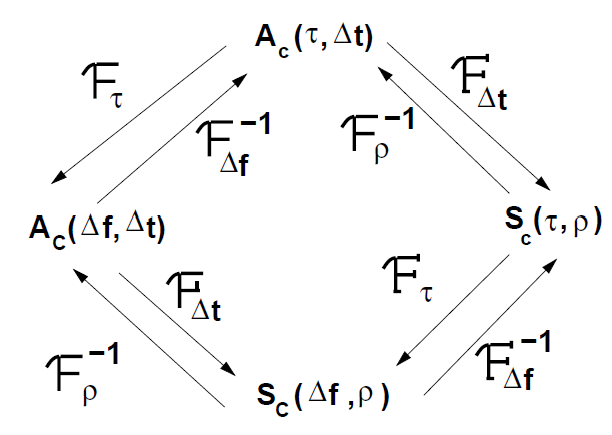
\includegraphics[width=\textwidth]{fig/fig29.png}
		\caption{Fourier Transform Relationships}
	\end{figure}
	
	Disse transformationer anvendes i praksis til at bestemme kanalens egenskaber såsom Doppler-spredning, forsinkelsesspredning og sammenhængende båndbredde. Ved at måle spredningsfunktionen \( S_c(\tau, \rho) \) kan man udlede kanalens vigtigste karakteristika og dermed optimere det trådløse kommunikationssystem.
	
	\section{Discrete-Time Model}	
	I analyse af trådløse kommunikationssystemer er det vigtigt at modellere kanalen på en måde, der afspejler de multipath-komponenter, som påvirker signalet under transmission. To vigtige modeller for dette er \textit{Point Scatterer Channel Model} og den tilsvarende diskrete tidsmodel.
	
	\subsection{Point Scatterer Channel Model}
	I en multipath-kanal består det modtagne signal af bidrag fra flere signalstier, som kan reflekteres, brydes eller spredes af objekter i miljøet. Dette er illustreret i \textit{Figur 3.16}, hvor forskellige objekter (f.eks. bygninger eller køretøjer) skaber flere refleksioner til modtageren. Den tilsvarende kanalimpulsrespons \(c(\tau; t)\) beskrives ved summen af bidragene fra \(N\) multipath-komponenter:
	
	\[
	c(\tau; t) = \sum_{n=0}^{N} \alpha_n(t) e^{-j \phi_n(t)} \delta(\tau - \tau_n(t)).
	\]
	
	Her repræsenterer \( \alpha_n(t) \) amplituden af den \(n\)-te komponent, \( \phi_n(t) \) er faseforskydningen, og \( \tau_n(t) \) er forsinkelsen på grund af den \(n\)-te signalsti. Kroneckerdeltafunktionen \( \delta(\tau - \tau_n(t)) \) angiver, at den \(n\)-te komponent ankommer ved forsinkelsen \( \tau_n(t) \).
	
	\begin{figure}[!h]
		\centering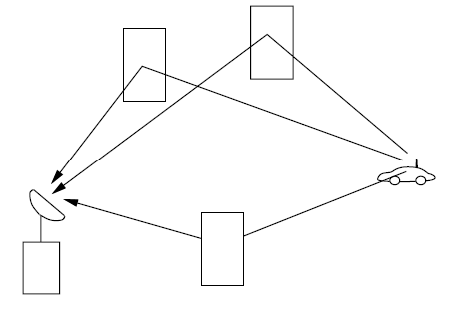
\includegraphics[width=\textwidth]{fig/fig30.png}
		\caption{Point Scatterer Channel Model}
	\end{figure}
	
	\subsection{Diskret tids approksimation}
	For at lette beregninger og analyse af multipath-kanaler, kan vi antage en diskret tidsmodel, hvor kanalens impulssvar \( c(\tau; t) \) samples ved bestemte tidspunkter. Denne diskretisering gør det muligt at opdele kanalen i \(M\) diskrete samples, som illustreret i \textit{Figur 3.17}. Hver sample \( r_m \) repræsenterer bidraget fra en multipath-komponent ved en bestemt forsinkelse \( mT \), hvor \(T\) er samplingintervallet.
	
	\begin{figure}[!h]
		\centering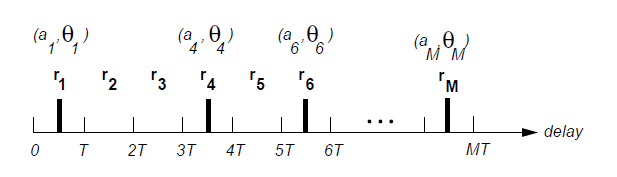
\includegraphics[width=\textwidth]{fig/fig31.png}
		\caption{Discrete Time Approximation}
	\end{figure}

	Hver sample \( r_m \) er relateret til en amplitude \( a_m \) og en fase \( \theta_m \), og tidsforsinkelsen mellem successive samples er \( T \). Dette gør det muligt at modellere kanalen som en sum af diskrete impulser, hvor hver impuls repræsenterer en refleksion fra et bestemt objekt i miljøet.
	\newline\newline
	Denne diskretisering bruges ofte i praksis til at simulere kanaler i trådløse systemer, hvor man ønsker at modellere de mange multipath-komponenter med begrænsede ressourcer. Den diskrete model gør det muligt at beregne kanalens effekt, forsinkelsesspredning og sammenhængende båndbredde mere effektivt.
	
	\section{Space-Time Channel Models}
	I moderne trådløse kommunikationssystemer er det vigtigt at modellere kanalen som en tids- og rumvarierende enhed for at kunne håndtere de mange multipath-komponenter, der kan opstå i en trådløs kanal. Disse modeller er særligt vigtige i systemer med flere antenner (MIMO), hvor både tid og rum bruges til at forbedre signalets kvalitet.
	\newline\newline
	Kanalimpulsresponsen \(c(\tau, t)\) for en space-time kanal kan udtrykkes som summen af bidrag fra \(N(t)\) multipath-komponenter:
	
	\[
	c(\tau, t) = \sum_{n=0}^{N(t)} \alpha_n(t) e^{-j \phi_n(t)} \bar{a}(\theta_n(t)) \delta(\tau - \tau_n(t)),
	\]
	
	hvor:
	\begin{itemize}
		\item \( \alpha_n(t) \) er amplituden af den \(n\)-te multipath-komponent,
		\item \( \phi_n(t) \) er den tilsvarende faseforskydning,
		\item \( \tau_n(t) \) er forsinkelsen for den \(n\)-te komponent,
		\item \( \theta_n(t) \) repræsenterer ankomstvinklen (Angle of Arrival, AoA) for den \(n\)-te komponent, og
		\item \( \bar{a}(\theta_n(t)) \) er antennemønsterets vektor for ankomstvinklen \( \theta_n(t) \).
	\end{itemize}

	Antennevektoren \( \bar{a}(\theta_n(t)) \) kan defineres som:
	
	\[
	\bar{a}(\theta_n(t)) = \left[ e^{-j \psi_{n,1}}, \ldots, e^{-j \psi_{n,M}} \right]^T,
	\]
	
	hvor \( \psi_{n,m} \) er faseforskydningen for antenneelementet \( m \) i et array af \( M \) antenneelementer.
	
	\subsection{Vinkelspredning og gennemsnitlig AoA}
	En vigtig parameter i Space-Time Channel Models er vinkelspredningen \( \sigma_{\theta} \), som beskriver variabiliteten af ankomstvinklerne i en multipath-kanal. Den gennemsnitlige ankomstvinkel \( \mu_{\theta} \) og vinkelspredningen \( \sigma_{\theta} \) kan beregnes som:
	
	\[
	\mu_{\theta} = \frac{\int_{-\pi}^{\pi} \theta A(\theta) d\theta}{\int_{-\pi}^{\pi} A(\theta) d\theta},
	\]
	
	\[
	\sigma_{\theta} = \sqrt{\frac{\int_{-\pi}^{\pi} (\theta - \mu_{\theta})^2 A(\theta) d\theta}{\int_{-\pi}^{\pi} A(\theta) d\theta}},
	\]
	
	hvor \( A(\theta) \) er fordelingsfunktionen for ankomstvinklerne. Disse ligninger er vigtige, fordi de beskriver spredningen af multipath-komponenterne i rummet, hvilket har direkte indflydelse på modtagersystemets evne til at udnytte rumlig diversitet.
	
	\subsection*{Space-Time model for MIMO-systemer}
	I et MIMO-system, hvor både afsendelse og modtagelse sker over flere antenner, bruges Space-Time Channel Models til at beskrive sammenhængen mellem hver antenneport og de forskellige multipath-komponenter. Impulsresponsen for et MIMO-system kan udtrykkes som en matrix, hvor hver matrixelement repræsenterer en kanal mellem en afsendende og en modtagende antenne.
	\newline\newline
	Denne formalisering giver mulighed for at analysere kanalens kapacitet, forsinkelsesspredning og rumlig diversitet, hvilket er essentielt for at designe trådløse systemer, der kan udnytte de rumlige dimensioner for at opnå højere datahastigheder og bedre signalmodtagelse.
	
	\chapter{Opgaver}
	\section{Exercises week 2}
	
	\begin{enumerate}
		\item Under the free-space path loss model, find the transmit power required to obtain a received power of 1 dBm for a wireless system with isotropic antennas ($G_t = G_r = 1$) and a carrier frequency $f_c = 5$ GHz, assuming a distance $d = 10$ m. Repeat for $d = 100$ m.
		\newline\newline\noindent
		\textbf{Solution:} We need to find the transmit power \( P_t \) required to achieve a received power \( P_r = 1 \, \text{dBm} \) for a wireless system with isotropic antennas \( (G_t = G_r = 1) \) and a carrier frequency \( f_c = 5 \, \text{GHz} \) at distances \( d = 10 \, \text{m} \) and \( d = 100 \, \text{m} \). Following is given:
		
		\begin{itemize}
			\item \(G_t = 1\)
			\item \(G_r = 1\)
			\item \(P_r = 1 dBm\)
			\item \(f_c = 5\times10^9\)
			\item \(d_{10m} = 10 m\)
			\item \(d_{100m} = 100 m\)
		\end{itemize}
		Calculating \(\lambda\) by:
		\[
			\lambda=\frac{c}{f_c}=\frac{3\times10^8}{5\times10^9}=0.06m
		\]
		The free-space path loss (FSPL) formula is given by:
		
		\[
			L_{FS}(dBm) = 20log\bigg(\frac{\lambda}{4\pi d}\bigg)=
		\]
		
		The Linkage Budge Model is given by:
		
		\[
		P_r (\text{dBm}) = P_t (\text{dBm}) + G_t (\text{dB}) + G_r (\text{dB}) - L (\text{dB})
		\]
		
		Where L(dB) is \(L_{FS}\)
		\newline\newline\noindent
		\[
			P_t(dBm)=P_r(dBm)-G_t(dB)-G_r(db)-L_{FS}(dBm)=
		\]
		\[
		P_t(dBm)=1-0-0-20log\frac{0.06}{40\pi}=
		\]
		
		
		\textbf{Final Answer:} The transmit power required for a received power of \( 1 \, \text{dBm} \) at \( d = 10 \, \text{m} \) is \( 36.42 \, \text{dBm} \) or \(4.385KW\), and at \( d = 100 \, \text{m} \) is \( 56.42 \, \text{dBm} \) or \(438.53KW\).
		
		\item For the two-ray model with transmitter-receiver separation $d = 100$ m, $h_t = 10$ m, and $h_r = 2$ m, find the delay spread between the two signals.
		\newline\newline\noindent\textbf{Solution:} In order to find the delay spread between the two signals we will be using \textit{Delay Spread in Two-Ray Model}
		
		\[
		\Delta \tau = \frac{|d_1 - d_2|}{c}
		\]
		where:
		\begin{itemize}
			\item \( d_1 = d \): the line-of-sight (LOS) distance between the transmitter and receiver,
			\item \( d_2 = \sqrt{d^2 + (h_t + h_r)^2} \): the non-LOS distance between the transmitter and receiver,
			\item \( c \): speed of light (\(3 \times 10^8\) m/s).
		\end{itemize}
		
		\[
		\Delta \tau = \frac{|d_1 - \sqrt{d^2 + (h_t + h_r)^2}|}{c}=
		\]
		\[\frac{100-\sqrt{100^2+(10+2)^2}}{3\times10^8}=2.39\times10^{-9}s\]
		\textbf{Final answer:} The delay spread between the two signals are \(2.39\) nano seconds
		
		\item Find the critical distance $d_c$ under the two-ray model for a large macrocell in a suburban area with the base station mounted on a tower or building ($h_t = 20$ m), the receivers at height $h_r = 3$ m, and $f_c = 2$ GHz. Is this a good size for cell radius in a suburban macrocell? Why or why not?
		\newline\newline
		\textbf{Solution:} Finding the \textit{The Critical Distance} \(d_c\) is done by:
		\[
		d_c = \frac{4 h_t h_r}{\lambda}=\frac{4\times20\text{m}\times3\text{m}}{\frac{3\times10^8\text{m}}{2\times10^9Hz}}=\frac{300\text{m}^2}{0.15\text{m}}=1.6\times10^{3}m
		\]
		\textbf{Final answer:} \textit{The Critical Distance} is calculated to be \(1600\text{m}\). It's difficult to answer if it's a good size or not because it is necessary to have knowledge about the environment, but normally cells in suburban areas they are between 1 - 3 km
		 
		\item Consider a receiver with noise power $-160$ dBm within the signal bandwidth of interest. Assume a single-slope path loss model with $d_0 = 1$ m, $K$ obtained from the free-space path loss formula with isotropic antennas and $f_c = 1$ GHz, and $\gamma = 4$. For a transmit power of $P_t = 10$ mW, find the maximum distance between the transmitter and receiver such that the received signal-to-noise power ratio is 20 dB.
		\newline\newline\noindent
		\textbf{Solution:} We are given the following parameters:
		\begin{itemize}
			\item Noise power \( P_n = -160 \, \text{dBm} \)
			\item Transmit power \( P_t = 10 \, \text{mW} = 10 \, \text{dBm} \)
			\item Reference distance \( d_0 = 1 \, \text{m} \)
			\item Carrier frequency \( f_c = 1 \, \text{GHz} \)
			\item Path loss exponent \( \gamma = 4 \)
			\item Signal-to-noise ratio (SNR) = 20 dB
		\end{itemize}
		
		We want to find the maximum distance \( d \) such that the received signal-to-noise ratio is 20 dB.
		
		\textbf{Step 1: Convert noise power from dBm to watts}\newline
		
		First, we need to convert the noise power from dBm to watts:
		\[
		P_n (\text{W}) = 10^{\frac{P_n (\text{dBm})}{10}} \times 10^{-3}
		\]
		Substituting \( P_n = -160 \, \text{dBm} \):
		\[
		P_n = 10^{\frac{-160}{10}} \times 10^{-3} = 10^{-16} \times 10^{-3} = 10^{-19} \, \text{W}
		\]
		
		\textbf{Step 2: Calculate free-space path loss at the reference distance \( d_0 \)}\newline
		
		The free-space path loss at the reference distance \( d_0 = 1 \, \text{m} \) is given by:
		\[
		L_{\text{FS}}(d_0) = 20 \log_{10} \left( \frac{4\pi d_0 f_c}{c} \right)
		\]
		where:
		\begin{itemize}
			\item \( d_0 = 1 \, \text{m} \),
			\item \( f_c = 1 \times 10^9 \, \text{Hz} \),
			\item \( c = 3 \times 10^8 \, \text{m/s} \).
		\end{itemize}
		
		Substituting these values:
		\[
		L_{\text{FS}}(d_0) = 20 \log_{10} \left( \frac{4 \pi \times 1 \times 10^9}{3 \times 10^8} \right)
		\]
		\[
		L_{\text{FS}}(d_0) = 20 \log_{10}(41.89) = 32.44 \, \text{dB}
		\]
		
		\textbf{Step 3: Use the single-slope path loss model}\newline
		
		The total path loss at a distance \( d \) is given by:
		\[
		L(d) = L(d_0) + 10 \gamma \log_{10} \left( \frac{d}{d_0} \right)
		\]
		Substituting \( L(d_0) = 32.44 \, \text{dB} \) and \( \gamma = 4 \), we get:
		\[
		L(d) = 32.44 + 40 \log_{10}(d)
		\]
		
		\textbf{Step 4: Calculate received power}
		
		The received power \( P_r \) can be calculated as:
		\[
		P_r (\text{dBm}) = P_t (\text{dBm}) - L(d)
		\]
		Substituting \( P_t = 10 \, \text{dBm} \):
		\[
		P_r = 10 - (32.44 + 40 \log_{10}(d)) = -22.44 - 40 \log_{10}(d)
		\]
		
		\textbf{Step 5: Apply the SNR condition}
		
		We know that:
		\[
		\text{SNR} = P_r (\text{dBm}) - P_n (\text{dBm})
		\]
		Substituting the given \( \text{SNR} = 20 \, \text{dB} \) and \( P_n = -160 \, \text{dBm} \):
		\[
		20 = P_r - (-160)
		\]
		\[
		P_r = -140 \, \text{dBm}
		\]
		
		\textbf{Step 6: Solve for \( d \)}
		
		Now we can solve for \( d \). From the equation for \( P_r \):
		\[
		-140 = -22.44 - 40 \log_{10}(d)
		\]
		Solving for \( \log_{10}(d) \):
		\[
		-140 + 22.44 = -40 \log_{10}(d)
		\]
		\[
		-117.56 = -40 \log_{10}(d)
		\]
		\[
		\log_{10}(d) = \frac{117.56}{40} \approx 2.939
		\]
		Now, solve for \( d \):
		\[
		d = 10^{2.939} \approx 870.1 \, \text{m}
		\]
		
		\textbf{Final answer}
		
		The maximum distance between the transmitter and receiver such that the received signal-to-noise ratio is 20 dB is approximately \( \mathbf{870.1 \, \text{m}} \).
		
		\item Table 2.7 lists a set of empirical path loss measurements. Assume a carrier frequency $f_c = 2$ GHz.
		
		\begin{enumerate}
			\item Find the parameters of a single-slope path loss model plus log-normal shadowing that best fit this data assuming $K$ is calculated from free-space path loss at the reference distance $d_r = 1$ m.
			
			\item Find the path loss at 2 Km based on this model.
			
			\item Find the outage probability at a distance $d$ assuming the received power at $d$ due to path loss alone is 10 dB above the required power for non-outage.
		\end{enumerate}
	\end{enumerate}
	
	\begin{table}[h!]
		\centering
		\caption{Path loss measurements for Problem 2-14}
		\begin{tabular}{|c|c|}
			\hline
			\textbf{Distance from Transmitter} & $\mathbf{\frac{P_r}{P_t}}$ \\
			\hline
			5 m   & $-60$ dB \\
			25 m  & $-80$ dB \\
			65 m  & $-105$ dB \\
			110 m & $-115$ dB \\
			400 m & $-135$ dB \\
			1000 m & $-150$ dB \\
			\hline
		\end{tabular}
	\end{table}
	\textbf{Solution:} \textbf{Problem Statement:} Table 2.7 lists a set of empirical path loss measurements. Assume a carrier frequency \( f_c = 2 \, \text{GHz} \).
	
	\begin{itemize}
		\item [(a)] Find the parameters of a single-slope path loss model plus log-normal shadowing that best fit this data assuming \( K \) is calculated from free-space path loss at the reference distance \( d_r = 1 \, \text{m} \).
		\item [(b)] Find the path loss at \( 2 \, \text{km} \) based on this model.
		\item [(c)] Find the outage probability at a distance \( d \) assuming the received power at \( d \) due to path loss alone is 10 dB above the required power for non-outage.
	\end{itemize}
	
	\textbf{Given Data:}
	
	The following path loss measurements are provided:
	
	\begin{table}[h!]
		\centering
		\begin{tabular}{|c|c|}
			\hline
			\textbf{Distance from Transmitter} & \textbf{Path Loss} (\( P_r / P_t \)) \\
			\hline
			5 m    & -60 dB \\
			25 m   & -80 dB \\
			65 m   & -105 dB \\
			110 m  & -115 dB \\
			400 m  & -135 dB \\
			1000 m & -150 dB \\
			\hline
		\end{tabular}
		\caption{Path loss measurements for Problem 2-14}
	\end{table}
	
	\textbf{Solution:} We will be using \textit{Single-slope path loss model} with \textit{log-normal shadowing}
	\newline\newline\noindent
	The single-slope path loss model is given by:
	\[
	L(d) = L(d_r) + 10 \gamma \log_{10} \left( \frac{d}{d_r} \right)
	\]
	where:
	\begin{itemize}
		\item \( L(d_r) \) is the path loss at the reference distance \( d_r = 1 \, \text{m} \),
		\item \( \gamma \) is the path loss exponent,
		\item \( d \) is the distance from the transmitter.
	\end{itemize}
	
	The constant \( K = L(d_r) \) can be computed from the free-space path loss formula:
	\[
	L_{\text{FS}}(d_r) = 20 \log_{10} \left( \frac{4\pi d_r f_c}{c} \right)
	\]
	Substituting \( d_r = 1 \, \text{m} \), \( f_c = 2 \, \text{GHz} = 2 \times 10^9 \, \text{Hz} \), and \( c = 3 \times 10^8 \, \text{m/s} \):
	\[
	L_{\text{FS}}(d_r) = 20 \log_{10} \left( \frac{4 \pi \times 1 \times 2 \times 10^9}{3 \times 10^8} \right)
	\]
	\[
	L_{\text{FS}}(d_r) = 20 \log_{10}(83.78) = 38.46 \, \text{dB}
	\]
	
	Next, using the provided data, we can apply regression to estimate \( \gamma \) and the shadowing effect by fitting the measured path loss data to the single-slope path loss model.
	\newline\newline\noindent
	\textbf{Path loss at 2 Km}
	\newline
	To find the path loss at \( d = 2 \, \text{km} = 2000 \, \text{m} \), we use the single-slope path loss model:
	\[
	L(2000) = L(d_r) + 10 \gamma \log_{10} \left( \frac{2000}{1} \right)
	\]
	Substituting \( L(d_r) = 38.46 \, \text{dB} \) and the value of \( \gamma \) estimated from part (a):
	\[
	L(2000) = 38.46 + 10 \gamma \log_{10}(2000)
	\]
	\noindent
	\textbf{Outage probability at a distance \( d \)}
	\newline
	The outage probability is calculated using log-normal shadowing. The outage probability is the probability that the received power falls below the required threshold for non-outage. Given that the received power at \( d \) is 10 dB above the required power, we use the following formula:
	\[
	P_{\text{out}} = Q \left( \frac{P_{\text{threshold}} - (P_t - L(d))}{\sigma} \right)
	\]
	where \( Q(x) \) is the Q-function, \( \sigma \) is the standard deviation of shadowing, and \( L(d) \) is the path loss at distance \( d \).
	
	\section*{Exercises week 3}
	
	\subsection*{3-3}
	Consider a time-invariant indoor wireless channel with LOS component at delay 23 ns, a multipath component at delay 48 ns, and another multipath component at delay 67 ns. 
	Find the delay spread assuming that the demodulator synchronizes to the LOS component. Repeat assuming that the demodulator synchronizes to the first multipath component.
	
	\subsection*{3-6}
	Assume a Rayleigh fading channel with average signal power \( 2\sigma^2 = -80 \, \text{dBm} \). What is the power outage probability of this channel relative to the threshold \( P_0 = -95 \, \text{dBm} \)? How about \( P_0 = -90 \, \text{dBm} \)?
	
	\subsection*{3-7}
	Suppose we have an application that requires a power outage probability of \( 0.01 \) for the threshold \( P_0 = -80 \, \text{dBm} \). For Rayleigh fading, what value of the average signal power is required?
	
	\subsection*{3-8}
	Assume a Rician fading channel with \( 2\sigma^2 = -80 \, \text{dBm} \) and a target power of \( P_0 = -80 \, \text{dBm} \). Find the outage probability assuming that the LOS component has average power \( s^2 = -80 \, \text{dBm} \).
	
	\subsection*{3-9}
	Consider a wideband channel with the multipath intensity profile:
	
	\[
	A_c(\tau) = 
	\begin{cases}
		e^{-\tau/0.0001} & 0 \leq \tau \leq 30 \, \mu s, \\
		0 & \text{else}.
	\end{cases}
	\]
	
	\begin{itemize}
		\item[(a)] What is the maximum delay of any non-LOS components in this case?
		\item[(b)] Find the average delay spread and RMS delay spread.
		\item[(c)] How should we select our symbol period in order to avoid ISI?
	\end{itemize}
	
	
	\part{Formula Collection}
	\chapter{Kapitel 2}
	\section{Path Loss Models}
	\subsection{Free-Space Path Loss (FSPL)}
	The free-space path loss (FSPL) represents the attenuation of a signal as it propagates in free space (without obstructions). It describes how the signal power diminishes due to the spreading of the wavefront over an expanding spherical surface.
	
	The FSPL is calculated by the formula:
	\[
	L_{\text{FS}}(\text{dB}) = 20 \log_{10} \left( \frac{4\pi d f_c}{c} \right)
	\]
	
	or
	
	\[
		FSPL = \bigg(\frac{4\pi df_c}{c}\bigg)^2
	\]
	where:
	\begin{itemize}
		\item \( d \) is the distance between the transmitter and the receiver (in meters),
		\item \( f_c \) is the carrier frequency (in Hz),
		\item \( c \) is the speed of light, \(c = 3 \times 10^8 \, \text{m/s}\).
	\end{itemize}
	
	The free-space path loss increases with both frequency and distance. Higher frequency signals and longer transmission distances experience greater path loss.
	
	\subsection{Received Power Calculation}
	
	The received power in a free-space environment can be calculated using the link budget equation. This relates the transmitted power, gains, and losses, such as free-space path loss:
	
	\[
	P_r (\text{dBm}) = P_t (\text{dBm}) + 10 \log_{10}(G_t) + 10 \log_{10}(G_r) - L_{\text{FS}} (\text{dB})
	\]
	where:
	\begin{itemize}
		\item \( P_r (\text{dBm}) \) is the received power (in dBm),
		\item \( P_t (\text{dBm}) \) is the transmitted power (in dBm),
		\item \( G_t \) is the gain of the transmitting antenna (in dB),
		\item \( G_r \) is the gain of the receiving antenna (in dB),
		\item \( L_{\text{FS}} (\text{dB}) \) is the free-space path loss.
	\end{itemize}
	
	\subsection{Simplified Form for Isotropic Antennas}
	
	For isotropic antennas, where \( G_t = G_r = 1 \) (i.e., 0 dB gain), the received power can be simplified as:
	
	\[
	P_r (\text{dBm}) = P_t (\text{dBm}) - L_{\text{FS}} (\text{dB})
	\]
	This simplifies the calculation when using omnidirectional antennas, where no directional gain is assumed.
	
	\subsection{Relationship Between Path Loss and Received Power}
	
	The free-space path loss can also be derived in terms of the ratio between transmitted and received power:
	\[
	P_L (\text{dB}) = 10 \log_{10} \left( \frac{P_t}{P_r} \right)
	\]
	Substituting \(L_{\text{FS}}\) into this equation gives:
	\[
	P_L (\text{dB}) = -10 \log_{10} \left( \frac{G_t G_r \lambda^2}{(4 \pi d)^2} \right)
	\]
	where:
	\begin{itemize}
		\item \( \lambda = \frac{c}{f_c} \) is the wavelength of the signal (in meters),
		\item \( G_t \) is the gain of the transmitter antenna (linear),
		\item \( G_r \) is the gain of the receiver antenna (linear).
	\end{itemize}
	
	This equation shows how the received power decreases as distance increases (proportional to \(d^2\)) and how higher frequencies (smaller \(\lambda\)) experience more path loss.
	
	\subsection{Importance of Antenna Gains}
	
	Antenna gains \( G_t \) and \( G_r \) play an important role in improving received power by focusing the signal energy in specific directions. In the case of directional antennas with higher gain, the received power increases, helping to compensate for higher path loss at greater distances or higher frequencies.
	
	\subsection{Free-Space Path Loss in dB}
	
	The free-space path loss in decibels for isotropic antennas can be expressed as:
	\[
	L_{\text{FS}} (\text{dB}) = -10 \log_{10} \left( \frac{G_t G_r \lambda^2}{(4 \pi d)^2} \right)
	\]
	
	Where:
	\begin{itemize}
		\item \( G_t \) and \( G_r \) are the transmitter and receiver antenna gains, respectively (in linear scale),
		\item \( \lambda \) is the wavelength (in meters),
		\item \( d \) is the distance between the transmitter and the receiver (in meters).
	\end{itemize}
	
	If \(G_t = G_r = 1\), this simplifies further to:
	\[
	L_{\text{FS}} (\text{dB}) = 20 \log_{10} \left( \frac{4 \pi d}{\lambda} \right)
	\]
	This form directly relates the path loss to the distance and wavelength.
	
	\subsection{Hata Model for Urban Areas}
	The Hata model for urban areas is given by:
	\[
	P_L(\text{dB}) = 69.55 + 26.16 \log_{10}(f_c) - 13.82 \log_{10}(h_t) - a(h_r) + \left( 44.9 - 6.55 \log_{10}(h_t) \right) \log_{10}(d)
	\]
	where:
	\begin{itemize}
		\item \( f_c \): carrier frequency (MHz),
		\item \( h_t \): height of the transmitter (meters),
		\item \( h_r \): height of the receiver (meters),
		\item \( d \): distance between transmitter and receiver (kilometers),
		\item \( a(h_r) \): correction factor for receiver height.
	\end{itemize}
	
	\subsection{Single-Slope Path Loss Model}
	The single-slope path loss model, with reference distance \(d_0\), is given by:
	\[
	L(d) (\text{dB}) = L(d_0) (\text{dB}) + 10 \gamma \log_{10} \left( \frac{d}{d_0} \right)
	\]
	where:
	\begin{itemize}
		\item \( L(d) \): path loss at distance \( d \) (dB),
		\item \( L(d_0) \): path loss at reference distance \( d_0 \) (dB),
		\item \( \gamma \): path loss exponent,
		\item \( d_0 \): reference distance (often 1 meter),
		\item \( d \): distance between transmitter and receiver (meters).
	\end{itemize}
	
	\subsection{Received Power in Free Space}
	The received power \(P_r(d)\) at distance \(d\) using isotropic antennas is given by:
	\[
	P_r(d) = P_t G_t G_r \left( \frac{\lambda}{4 \pi d} \right)^2
	\]
	where:
	\begin{itemize}
		\item \( P_r(d) \): received power at distance \( d \) (W),
		\item \( P_t \): transmitted power (W),
		\item \( G_t \): gain of transmitting antenna (linear),
		\item \( G_r \): gain of receiving antenna (linear),
		\item \( \lambda = \frac{c}{f_c} \): wavelength (meters),
		\item \( d \): distance between transmitter and receiver (meters),
		\item \( c \): speed of light (\( 3 \times 10^8 \, \text{m/s} \)),
		\item \( f_c \): carrier frequency (Hz).
	\end{itemize}
	
	\subsection{Signal-to-Noise Ratio (SNR)}
	The signal-to-noise ratio (SNR) at the receiver is given by:
	\[
	SNR = \frac{P_r}{P_n}
	\]
	where:
	\begin{itemize}
		\item \( P_r \): received power (W),
		\item \( P_n \): noise power (W).
	\end{itemize}
	
	The noise power \( P_n \) is calculated as:
	\[
	P_n = N_0 B
	\]
	where:
	\begin{itemize}
		\item \( N_0 \): noise power spectral density (W/Hz),
		\item \( B \): system bandwidth (Hz).
	\end{itemize}
	
	\subsection{Maximum Distance for Given SNR}
	The maximum distance \(d_{\text{max}}\) such that the received SNR meets a target value \(SNR_{\text{target}}\) is given by rearranging the SNR formula:
	\[
	d_{\text{max}} = d_0 \cdot 10^{\frac{L(d_0) + 10 \log_{10} \left( \frac{P_t}{P_n} \right) - SNR_{\text{target}}}{10 \gamma}}
	\]
	where:
	\begin{itemize}
		\item \( d_{\text{max}} \): maximum distance between transmitter and receiver (meters),
		\item \( L(d_0) \): path loss at reference distance \(d_0\) (dB),
		\item \( P_t \): transmitted power (W),
		\item \( P_n \): noise power (W),
		\item \( SNR_{\text{target}} \): target SNR (dB),
		\item \( \gamma \): path loss exponent.
	\end{itemize}
	
	\subsection{COST 231 Model (Extension of Hata Model)}
	The COST 231 model for urban environments is given by:
	\[
	P_L(\text{dB}) = 46.3 + 33.9 \log_{10}(f_c) - 13.82 \log_{10}(h_t) - a(h_r) + \left( 44.9 - 6.55 \log_{10}(h_t) \right) \log_{10}(d) + C_M
	\]
	where:
	\begin{itemize}
		\item \( f_c \): carrier frequency (MHz),
		\item \( h_t \): height of the transmitter (meters),
		\item \( h_r \): height of the receiver (meters),
		\item \( d \): distance between transmitter and receiver (kilometers),
		\item \( C_M \): 0 dB for metropolitan areas, 3 dB for suburban areas.
	\end{itemize}
	
	\subsection{Two-Ray Ground Reflection Model}
	The received power using the two-ray model is:
	\[
	P_r = P_t \left[ \frac{\lambda}{4 \pi} \left( \frac{1}{d_1} + \frac{R}{d_2} \right) \right]^2
	\]
	where:
	\begin{itemize}
		\item \( P_r \): received power (W),
		\item \( P_t \): transmitted power (W),
		\item \( d_1, d_2 \): distances for line-of-sight and reflected paths (meters),
		\item \( R \): reflection coefficient (dimensionless),
		\item \( \lambda \): wavelength (meters).
	\end{itemize}
	
	\subsection{Critical Distance in Two-Ray Model}
	The critical distance \( d_c \) is given by:
	\[
	d_c = \frac{4 h_t h_r}{\lambda}
	\]
	where:
	\begin{itemize}
		\item \( h_t \): height of the transmitter (meters),
		\item \( h_r \): height of the receiver (meters),
		\item \( \lambda \): wavelength (meters).
	\end{itemize}
	
	\subsection{Delay Spread in Two-Ray Model}
	The delay spread \( \Delta \tau \) in the two-ray model is given by:
	\[
	\Delta \tau = \frac{|d_1 - d_2|}{c}
	\]
	where:
	\begin{itemize}
		\item \( d_1 = d \): the line-of-sight (LOS) distance between the transmitter and receiver (meters),
		\item \( d_2 = \sqrt{d^2 + (h_t + h_r)^2} \): the non-LOS distance between the transmitter and receiver (meters),
		\item \( c \): speed of light (\(3 \times 10^8\) m/s).
	\end{itemize}
	
	\section{Outage Probability}
	
	\subsection{Outage Probability under Path Loss and Shadowing}
	The outage probability \( P_{\text{out}} \) is defined as:
	\[
	P_{\text{out}} = 1 - Q \left( \frac{P_{\min} - (P_t - L_{\text{PL}}(d))}{\sigma_{\psi}} \right)
	\]
	where:
	\begin{itemize}
		\item \( P_{\min} \): minimum received power (W),
		\item \( L_{\text{PL}}(d) \): path loss at distance \( d \) (dB),
		\item \( \sigma_{\psi} \): standard deviation of shadowing (dB),
		\item \( Q(x) \): Q-function.
	\end{itemize}
	
	\section{Link Budget Equation}
	
	The link budget is calculated as:
	\[
	P_r (\text{dBm}) = P_t (\text{dBm}) + G_t (\text{dB}) + G_r (\text{dB}) - L (\text{dB})
	\]
	where:
	\begin{itemize}
		\item \( P_r \): received power (dBm),
		\item \( P_t \): transmitted power (dBm),
		\item \( G_t, G_r \): transmitter and receiver antenna gains (dB),
		\item \( L \): total loss (dB).
	\end{itemize}
	
	\section{Doppler Shift}
	
	The Doppler shift \( f_D \) is given by:
	\[
	f_D = \frac{v \cos \theta}{\lambda}
	\]
	where:
	\begin{itemize}
		\item \( v \): velocity of the receiver (m/s),
		\item \( \theta \): angle between movement direction and wavefront (radians),
		\item \( \lambda \): wavelength (meters).
	\end{itemize}
	
	\section{Probability and Fading}
	
	\subsection{Rayleigh Fading}
	
	The probability density function for Rayleigh fading is:
	\[
	f(r) = \frac{r}{\sigma^2} \exp \left( - \frac{r^2}{2\sigma^2} \right)
	\]
	where:
	\begin{itemize}
		\item \( r \): signal amplitude,
		\item \( \sigma^2 \): variance.
	\end{itemize}
	
	\subsection{Rician Fading}
	The probability density function for Rician fading is:
	\[
	f(r) = \frac{r}{\sigma^2} \exp \left( -\frac{r^2 + A^2}{2\sigma^2} \right) I_0 \left( \frac{Ar}{\sigma^2} \right)
	\]
	where:
	\begin{itemize}
		\item \( A \): peak amplitude of the line-of-sight component,
		\item \( I_0 \): modified Bessel function of the first kind.
	\end{itemize}
	
	\subsection{Simplified Path Loss Model for SNR}
	The simplified path loss model for Signal-to-Noise Ratio (SNR) is given by:
	\[
	SNR = \frac{P_t G_t G_r}{L N_0}
	\]
	where:
	\begin{itemize}
		\item \( P_t \): transmitted power (W),
		\item \( G_t, G_r \): transmitter and receiver antenna gains (linear),
		\item \( L \): total path loss (linear),
		\item \( N_0 \): noise power (W).
	\end{itemize} 
	
	\chapter{Kapitel 3}
	\section{Formelsamling for Statistical Multipath Channel Models}
	
	\subsection{Tidsvarierende Kanalimpulsrespons}
	
	\subsubsection{Matematisk Modellering af Tidsvarierende Kanalimpulsrespons}
	Kanalimpulsresponsen kan udtrykkes som en sum af \( N \) multipath-komponenter:
	
	\[
	c(\tau, t) = \sum_{n=0}^{N(t)} \alpha_n(t) e^{-j \phi_n(t)} \delta(\tau - \tau_n(t)),
	\]
	
	hvor \( \alpha_n(t) \) er amplituden, \( \phi_n(t) \) er fasen, og \( \tau_n(t) \) er forsinkelsen for den \(n\)-te komponent.
	
	\subsubsection{Kanalimpulsrespons ved Forskellige Tidspunkter}
	Kanalens impulssvar kan variere over tid. Autokorrelationsfunktionen for kanalen kan udtrykkes som:
	
	\[
	R_c(\tau, \Delta t) = \mathbb{E}[c^*(t) c(t + \Delta t)].
	\]
	
	\subsubsection{Tidsvarierende Kanalrespons i Frekvensdomænet}
	Frekvenskorrelationsfunktionen \( A_c(\Delta f, \Delta t) \) er relateret til impulssvaret gennem Fourier-transformation:
	
	\[
	A_c(\Delta f, \Delta t) = \int_{-\infty}^{\infty} A_c(\tau, \Delta t) e^{-j 2 \pi \Delta f \tau} d\tau.
	\]
	
	\subsubsection{Doppler-effekter}
	Doppler-frekvensen \( f_D \) kan beregnes som:
	
	\[
	f_D = \frac{v f_c}{c},
	\]
	
	hvor \( v \) er bevægelseshastigheden, \( f_c \) er bærefrekvensen, og \( c \) er lysets hastighed.
	
	\subsubsection{Kanalens Ikke-Stationære Respons}
	Kanalens ikke-stationære respons kan modelleres ved hjælp af autokorrelationsfunktionen:
	
	\[
	R_c(\tau, \Delta t) = \mathbb{E}[c^*(\tau, t) c(\tau, t + \Delta t)].
	\]
	
	\subsection{Narrow Fading Models}
	\subsubsection{In-Phase og Quadrature Komponenter}
	For fading kan kanalen opdeles i in-phase og quadrature-komponenter, hvor signalet kan skrives som:
	
	\[
	r(t) = I(t) \cos(2 \pi f_c t) - Q(t) \sin(2 \pi f_c t),
	\]
	
	hvor \( I(t) \) og \( Q(t) \) er henholdsvis in-phase og quadrature-komponenter.
	
	\subsubsection{Fading og Statistik}
	Fading beskrives ofte ved statistiske fordelinger såsom Rayleigh og Rician. Den gennemsnitlige effekt i et fading-miljø kan beregnes som:
	
	\[
	\bar{P} = \int_0^\infty p(r) r^2 dr,
	\]
	
	hvor \( p(r) \) er fordelingsfunktionen for amplitude \( r \).
	
	\subsubsection{Autokorrelation, Krydskorrelation og Spektraltæthed}
	Autokorrelationsfunktionen for fading-signaler er givet ved:
	
	\[
	R_{XX}(\tau) = \mathbb{E}[X(t) X^*(t + \tau)].
	\]
	
	Spektraltætheden \( S_{XX}(f) \) opnås ved Fourier-transformation af autokorrelationsfunktionen.
	
	\subsection{Envelope and Power Distributions}
	\subsubsection{Rayleigh-fordeling af Effekt}
	Rayleigh-fordelingen bruges til at beskrive fading i miljøer med mange multipath-komponenter og kan beskrives ved:
	
	\[
	p(r) = \frac{r}{\sigma^2} e^{-r^2 / (2 \sigma^2)}, \quad r \geq 0.
	\]
	
	\subsubsection{Rician Fading}
	Rician fading inkluderer en line-of-sight (LOS)-komponent og er givet ved:
	
	\[
	p(r) = \frac{r}{\sigma^2} e^{-(r^2 + s^2) / (2 \sigma^2)} I_0\left(\frac{r s}{\sigma^2}\right),
	\]
	
	hvor \( s \) er styrken af LOS-komponenten og \( I_0(\cdot) \) er modificeret Bessel-funktion af første orden.
	
	\subsubsection{Nakagami Fading}
	Nakagami-fordelingen beskrives ved:
	
	\[
	p(r) = \frac{2 m^m r^{2m-1}}{\Gamma(m) \Omega^m} e^{-\frac{m r^2}{\Omega}},
	\]
	
	hvor \( m \) er fading-parametret og \( \Omega \) er den gennemsnitlige effekt.
	
	\subsection{Wideband Fading Models}
	\subsubsection{Matematisk Modellering}
	Wideband fading modelleres ofte ved at analysere forsinkelsesspredning og koherensbåndbredde. Den gennemsnitlige forsinkelse \( T_m \) kan udtrykkes som:
	
	\[
	T_m = \frac{\int_0^\infty P_h(\tau) \tau d\tau}{\int_0^\infty P_h(\tau) d\tau},
	\]
	
	hvor \( P_h(\tau) \) er power delay profile (PDP).
	
	\subsubsection{Coherence Bandwidth}
	Sammenhængende båndbredde \( B_c \) kan relateres til forsinkelsesspredningen \( S_\tau \) ved:
	
	\[
	B_c \approx \frac{1}{2 \pi S_\tau}.
	\]
	
	\subsubsection{Doppler Power Spectrum and Channel Coherence Time}
	Koherenstiden \( T_c \), som er relateret til Doppler-frekvensen, kan beregnes som:
	
	\[
	T_c \approx \frac{1}{f_D}.
	\]
	
	\subsection{Discrete-Time Model}
	\subsubsection*{Point Scatterer Channel Model}
	Den diskrete kanalimpulsrespons i en point scatterer model er givet ved:
	
	\[
	c(\tau, t) = \sum_{n=0}^{N(t)} \alpha_n(t) e^{-j \phi_n(t)} \delta(\tau - \tau_n(t)).
	\]
	
	\subsection{Space-Time Channel Models}
	\subsubsection{Vinkelspredning og Gennemsnitlig AoA}
	Den gennemsnitlige ankomstvinkel \( \mu_\theta \) og vinkelspredningen \( \sigma_\theta \) kan beregnes som:
	
	\[
	\mu_\theta = \frac{\int_{-\pi}^{\pi} \theta A(\theta) d\theta}{\int_{-\pi}^{\pi} A(\theta) d\theta},
	\]
	
	\[
	\sigma_\theta = \sqrt{\frac{\int_{-\pi}^{\pi} (\theta - \mu_\theta)^2 A(\theta) d\theta}{\int_{-\pi}^{\pi} A(\theta) d\theta}}.
	\]
	
	\subsection{Forsinkelsesspredning (Delay Spread)}
	Forsinkelsesspredning er et mål for variationen i ankomsttidspunkter af multipath-komponenter. Følgende formler kan anvendes:
	
	\begin{itemize}
		\item \textbf{Gennemsnitlig forsinkelse} \( T_m \):
	
	\[
	T_m = \frac{\int_0^\infty P_h(\tau) \tau d\tau}{\int_0^\infty P_h(\tau) d\tau}
	\]
	
	\item  \textbf{RMS forsinkelsesspredning} \( S_\tau \):
	
	\[
	S_\tau = \sqrt{\frac{\int_0^\infty P_h(\tau) \tau^2 d\tau}{\int_0^\infty P_h(\tau) d\tau} - T_m^2}
	\]
	\end{itemize}
	
	For at undgå intersymbolinterferens (ISI) skal symbolperioden \( T_s \) være større end \( S_\tau \):
	
	\[
	T_s > S_\tau
	\]
	
	\subsection{Rayleigh Fading}
	\subsubsection{Power Outage Probability under Rayleigh Fading}
	For en Rayleigh fading kanal er outage probability \( P_\text{out} \) givet ved:
	
	\[
	P_\text{out} = 1 - \exp\left(-\frac{P_0}{2\sigma^2}\right)
	\]
	
	hvor:
	\begin{itemize}
		\item \( P_0 \) er tærskelværdien,
		\item \( 2\sigma^2 \) er den gennemsnitlige
	\end{itemize} effekt.
	
	\subsubsection{Bestemmelse af Gennemsnitlig Effekt for Givet Outage Probability}
	Hvis outage probability \( P_\text{out} \) er kendt, kan den gennemsnitlige effekt \( 2\sigma^2 \) beregnes ved at omarrangere formlen for outage probability:
	
	\[
	P_\text{out} = 1 - \exp\left(-\frac{P_0}{2\sigma^2}\right)
	\]
	
	Ved at sætte \( P_\text{out} = 0.01 \) og kende \( P_0 \), kan du finde \( 2\sigma^2 \).
	
	\subsection{Rician Fading}
	
	\subsubsection{Outage Probability for Rician Fading}
	For Rician fading er outage probability \( P_\text{out} \) givet ved:
	
	\[
	P_\text{out} = 1 - Q_1\left(\sqrt{\frac{2s^2}{2\sigma^2}}, \sqrt{\frac{2P_0}{2\sigma^2}}\right)
	\]
	
	hvor:
	\begin{itemize}
		\item \( s^2 \) er LOS-komponentens gennemsnitlige effekt,
		\item \( 2\sigma^2 \) er variansen af de ikke-LOS-komponenter,
		\item \( Q_1 \) er den modificerede Bessel-funktion af første orden.
	\end{itemize}
	
	\end{document}